\documentclass[14pt,a4paper]{extarticle}

\usepackage[T2A]{fontenc}
\usepackage[utf8]{inputenc}
\usepackage[russian]{babel}
\usepackage{geometry}
\usepackage{setspace}
\usepackage{graphicx}
\usepackage{float}
\usepackage{booktabs}
\usepackage{longtable}
\usepackage{array}
\usepackage{amsmath}
\usepackage{amssymb}
\usepackage{caption}
\usepackage{listings}
\usepackage{xcolor}
\usepackage{hyperref}
\usepackage{pdflscape}
\usepackage{indentfirst}

\geometry{left=30mm,right=15mm,top=20mm,bottom=20mm}
\onehalfspacing
\setlength{\parindent}{1.25cm}
\setlength{\parskip}{0pt}
\graphicspath{{coursework_doc_assets/}{figures/}{../reports/figures/}{../output/artifacts/stage5_improved/}{../output/artifacts/stage5_improved_augmented/}{../output/artifacts/stage5_attention/}}

\hypersetup{
    colorlinks=true,
    linkcolor=blue,
    citecolor=blue,
    urlcolor=blue,
    pdfauthor={\StudentName},
    pdftitle={Курсовая работа по дисциплине «Интеллектуальный анализ данных на основе методов машинного обучения»}
}

\providecommand{\StudentName}{Студент}
\providecommand{\StudentGroup}{4232}
\providecommand{\TeacherName}{В.Ю. Скобцов}
\providecommand{\TeacherTitle}{канд.\ техн. наук, доцент}
\providecommand{\CourseTitle}{Интеллектуальный анализ данных на основе методов машинного обучения}
\providecommand{\WorkTitle}{Интеллектуальный анализ телеметрии малого космического аппарата и классификация штатных и нештатных состояний на основе методов машинного обучения}
\providecommand{\WorkYear}{2026}

\lstset{
    basicstyle=\ttfamily\small,
    breaklines=true,
    frame=single,
    backgroundcolor=\color{black!2},
    rulecolor=\color{black!25}
}

\begin{document}

\begin{titlepage}
\begin{center}
МИНИСТЕРСТВО НАУКИ И ВЫСШЕГО ОБРАЗОВАНИЯ РОССИЙСКОЙ ФЕДЕРАЦИИ\\
федеральное государственное автономное образовательное учреждение высшего образования\\
«САНКТ-ПЕТЕРБУРГСКИЙ ГОСУДАРСТВЕННЫЙ УНИВЕРСИТЕТ АЭРОКОСМИЧЕСКОГО ПРИБОРОСТРОЕНИЯ»\\
\textbf{КАФЕДРА 43}
\end{center}

\vspace{1.5cm}

\noindent\begin{tabular}{p{0.43\textwidth}p{0.5\textwidth}}
\textbf{КУРСОВАЯ РАБОТА} & \textbf{ЗАЩИЩЕНА С ОЦЕНКОЙ} \\
по дисциплине & \rule{0.42\textwidth}{0.4pt} \\
\textit{\CourseTitle} & подпись, дата \\
\end{tabular}

\vspace{1.2cm}

\begin{center}
\textbf{Тема:} \\
\textbf{\WorkTitle}
\end{center}

\vfill

\noindent\begin{tabular}{p{0.47\textwidth}p{0.47\textwidth}}
\textbf{ПРЕПОДАВАТЕЛЬ} & \textbf{РАБОТУ ВЫПОЛНИЛ} \\
\TeacherTitle & студент гр. № \StudentGroup \\
\rule{0.42\textwidth}{0.4pt} & \rule{0.42\textwidth}{0.4pt} \\
подпись, дата & подпись, дата \\
\TeacherName & \StudentName \\
инициалы, фамилия & инициалы, фамилия \\
\end{tabular}

\vspace{2cm}

\begin{center}
Санкт-Петербург \WorkYear
\end{center}
\end{titlepage}

\tableofcontents
\clearpage
\listoffigures
\clearpage
\listoftables
\clearpage

\section{Введение}
Курсовая работа посвящена построению и анализу прикладной системы интеллектуальной обработки телеметрии малого космического аппарата. Практическая цель исследования состоит в том, чтобы по последовательностям измерений датчиков отличать штатный режим эксплуатации от двух видов нештатных состояний: отказа и сбоя. Такая постановка непосредственно связана с задачами оперативного мониторинга, раннего выявления деградации бортовых систем и сокращения времени реакции оператора на аномальное поведение технического объекта.

Актуальность темы определяется тремя факторами. Во-первых, телеметрические данные являются многомерными, шумными и нестационарными; классические пороговые правила в таком контуре быстро упираются в предел точности. Во-вторых, распределение состояний аппарата несимметрично: подавляющее большинство наблюдений относится к штатному режиму, а редкие критические события представлены существенно меньшим числом примеров. В-третьих, инженерная ценность решения определяется не только итоговой метрикой, но и воспроизводимостью эксперимента, корректным временным разбиением без утечки и возможностью объяснить, почему модель принимает то или иное решение.

В работе реализован полный вычислительный контур: загрузка и валидация данных, разведочный анализ, подготовка окон фиксированной длины, обучение базовых и нейросетевых моделей, генетический поиск гиперпараметров, предобучение автоэнкодера, финальная оценка на отложенной тестовой части и оформление результатов в виде воспроизводимого отчёта. Дополнительно, в рамках улучшения проекта, были интегрированы следующие элементы: расчёт и визуализация ROC AUC, графики обучения, анализ важности признаков, аугментация временных окон, сравнение рекуррентных слоёв различных типов, исследование механизма внимания и контейнеризация запуска.

\section{Задание на курсовую работу}
Целью курсовой работы является разработка и исследование системы классификации состояний космического аппарата по телеметрическим данным на основе методов машинного обучения и глубоких нейронных сетей.

Для достижения поставленной цели были решены следующие задачи:
\begin{enumerate}
    \item сформирован и зафиксирован контракт данных, определяющий формат входных файлов, схему признаков, допустимые метки, правила обработки пропусков и параметры временного окна;
    \item выполнен разведочный анализ данных с оценкой объёма выборки, дисбаланса классов, выбросов и корреляционной структуры признаков;
    \item реализована подготовка двух версий признакового пространства: базовой (raw) и улучшенной (improved), включая median-импутацию, winsorization и робастное масштабирование;
    \item построены и сравнены baseline-модели, гибридные нейросетевые архитектуры и варианты с различными типами рекуррентного слоя;
    \item выполнен генетический поиск гиперпараметров и исследована устойчивость лучшей конфигурации;
    \item проведено предобучение автоэнкодера на неразмеченной телеметрии и сравнение с обучением классификатора «с нуля»;
    \item организовано воспроизводимое окружение эксперимента, включая фиксацию конфигурации, контроль версий библиотек, контрольные суммы датасетов и Docker-описание проекта;
    \item подготовлена аналитическая записка с таблицами, графиками, схемами, формулами и приложениями с кодом.
\end{enumerate}

\section{Исходные данные и постановка задачи}\label{sec:data}
В качестве размеченной части использовалась таблица \texttt{data/MKA\_TMI\_labels.xls}, содержащая 2679 строк и 50 столбцов, где 49 столбцов представляют числовые телеметрические признаки, а столбец \texttt{Class} хранит целевую метку. Неразмеченная часть представлена файлом \texttt{data/MKA\_04.2015\_unlabeled.csv} объёмом 15243 строки и 49 признаков. Вся обработка выполняется без привлечения внешних наборов данных; это соответствует академическому требованию использовать локально выданный преподавателем материал.

Задача решается в мультиклассовой постановке:
\begin{equation}
    y \in \{0,1,2\},
\end{equation}
где $0$ соответствует штатному режиму, $1$ --- отказу, а $2$ --- сбою.

Распределение классов в размеченном наборе следующее: 2356 наблюдений для класса 0, 218 наблюдений для класса 1 и 105 наблюдений для класса 2. Таким образом, отношение мощности мажоритарного и миноритарного классов составляет $2356 / 105 \approx 22{,}44$, что указывает на выраженный дисбаланс и требует использования метрик, устойчивых к смещению по частотам.

Разбиение на \texttt{train/val/test} выполнено строго по времени в пропорции 70/15/15 без случайного перемешивания окон. Для формирования обучающих примеров используется скользящее окно длины $T=128$ шагов со сдвигом $s=32$ шага. Соответственно, одно окно представляет собой трёхмерный тензор:
\begin{equation}
    X^{(i)} \in \mathbb{R}^{128 \times 49}.
\end{equation}

\begin{figure}[H]
\centering

\includegraphics[width=0.95\textwidth]{split_scheme.png}
\caption{Схема временного разбиения исходного ряда на обучающую, валидационную и тестовую части}
\end{figure}

\begin{figure}[H]
\centering

\includegraphics[width=0.72\textwidth]{class_distribution.png}
\caption{Распределение классов в размеченном наборе данных}
\end{figure}

\section{Разведочный анализ данных}\label{sec:eda}
Разведочный анализ показал, что явных пропусков после применения фиксированного списка null-токенов в исходных таблицах не осталось. Это означает, что основная сложность связана не с очисткой пустых значений, а с дисбалансом классов, выбросами и корректным временным протоколом валидации.

Наиболее выраженные выбросы по критерию межквартильного размаха наблюдаются у признаков \texttt{Ibs,A}, \texttt{TR1,C}, \texttt{Ipt1,A}, \texttt{Ubs,V}, \texttt{TDS2,C}. Для таких признаков доля значений, выходящих за стандартные IQR-границы, достигает 10--24\%, что указывает на тяжёлые хвосты и повышенную чувствительность моделей к экстремальным отсчётам. По этой причине в улучшенном варианте предобработки используется winsorization по квантилям 0.01 и 0.99.

Сильных парных корреляций уровня $|r|\ge 0.95$ обнаружено не было. Это означает, что набор признаков не содержит очевидных дублей, однако наличие умеренных корреляций всё равно требует осторожной интерпретации важности коэффициентов и нейросетевых весов.

\begin{figure}[H]
\centering
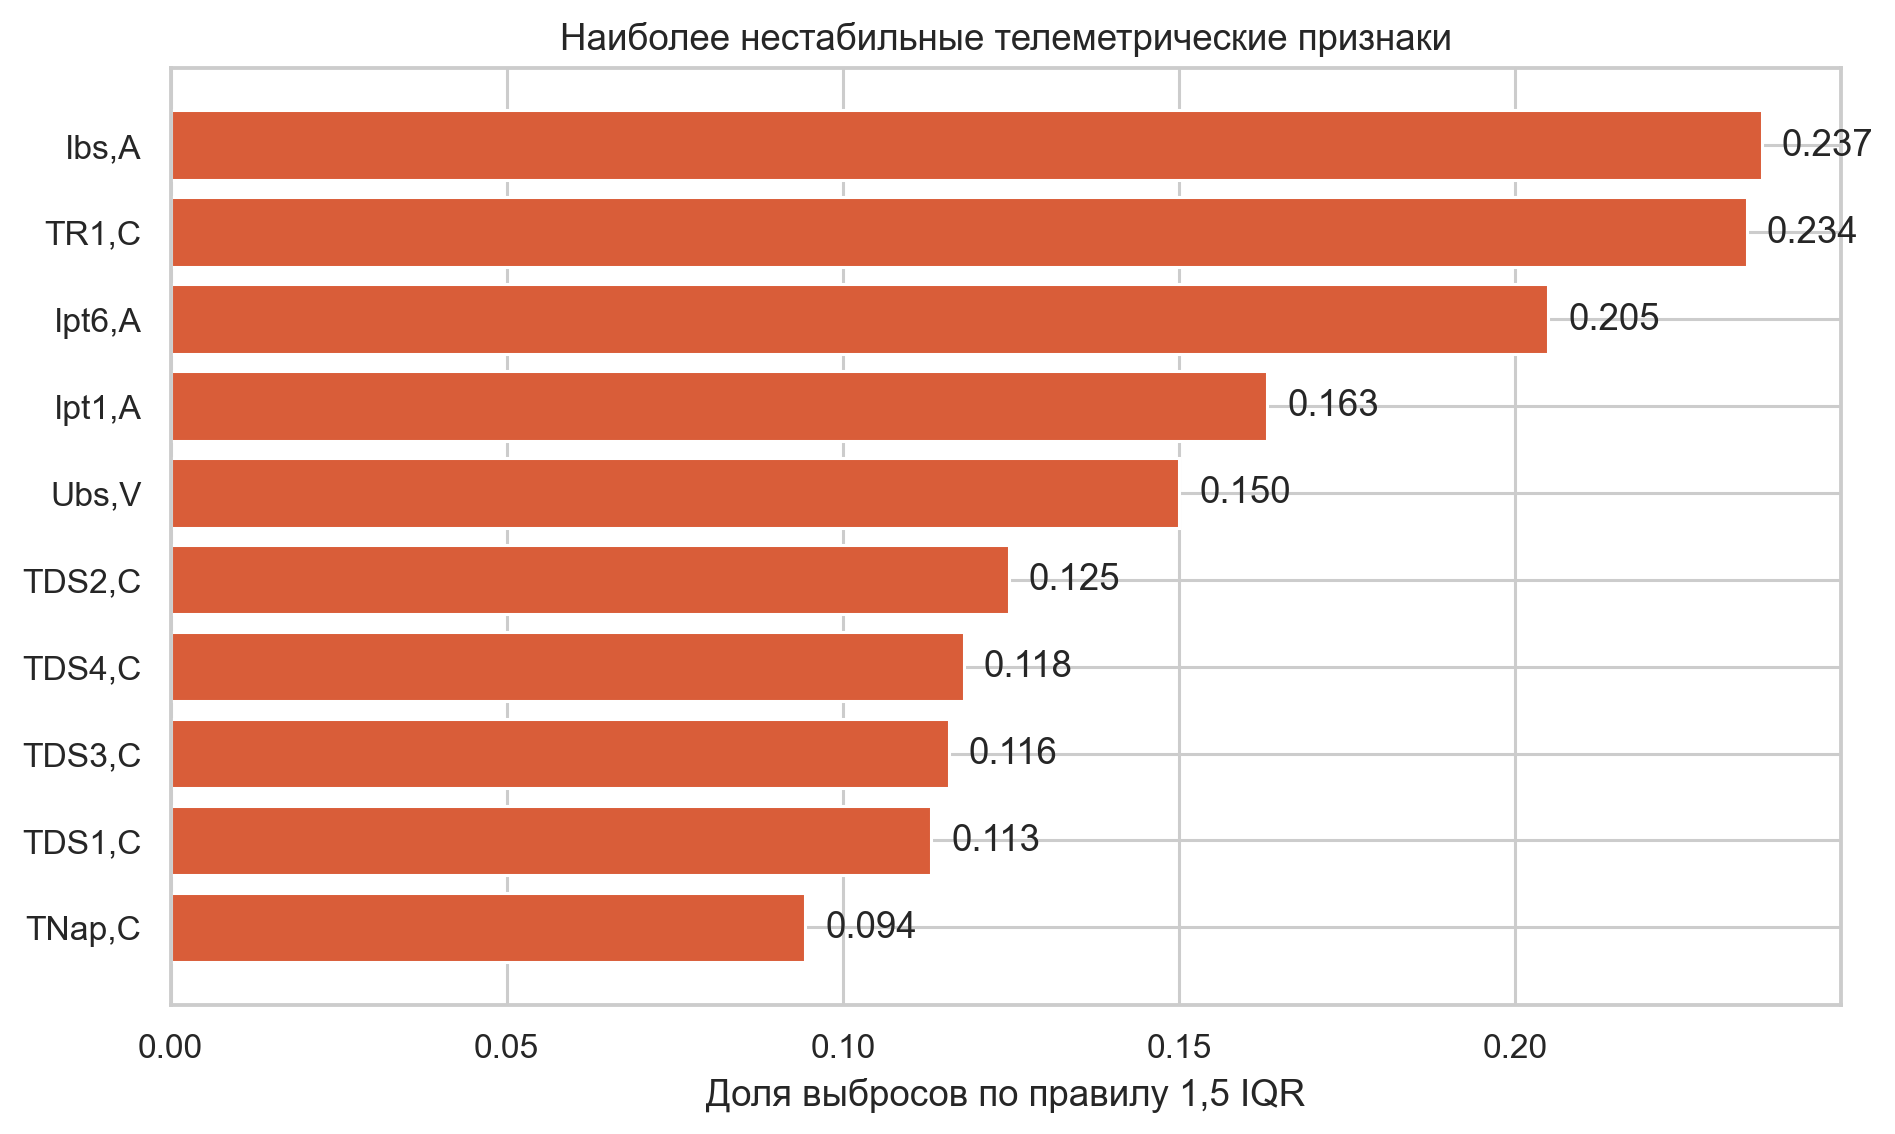
\includegraphics[width=0.82\textwidth]{outlier_shares.png}
\caption{Доли выбросов для признаков с наибольшей нестабильностью распределений}
\end{figure}

\begin{figure}[H]
\centering
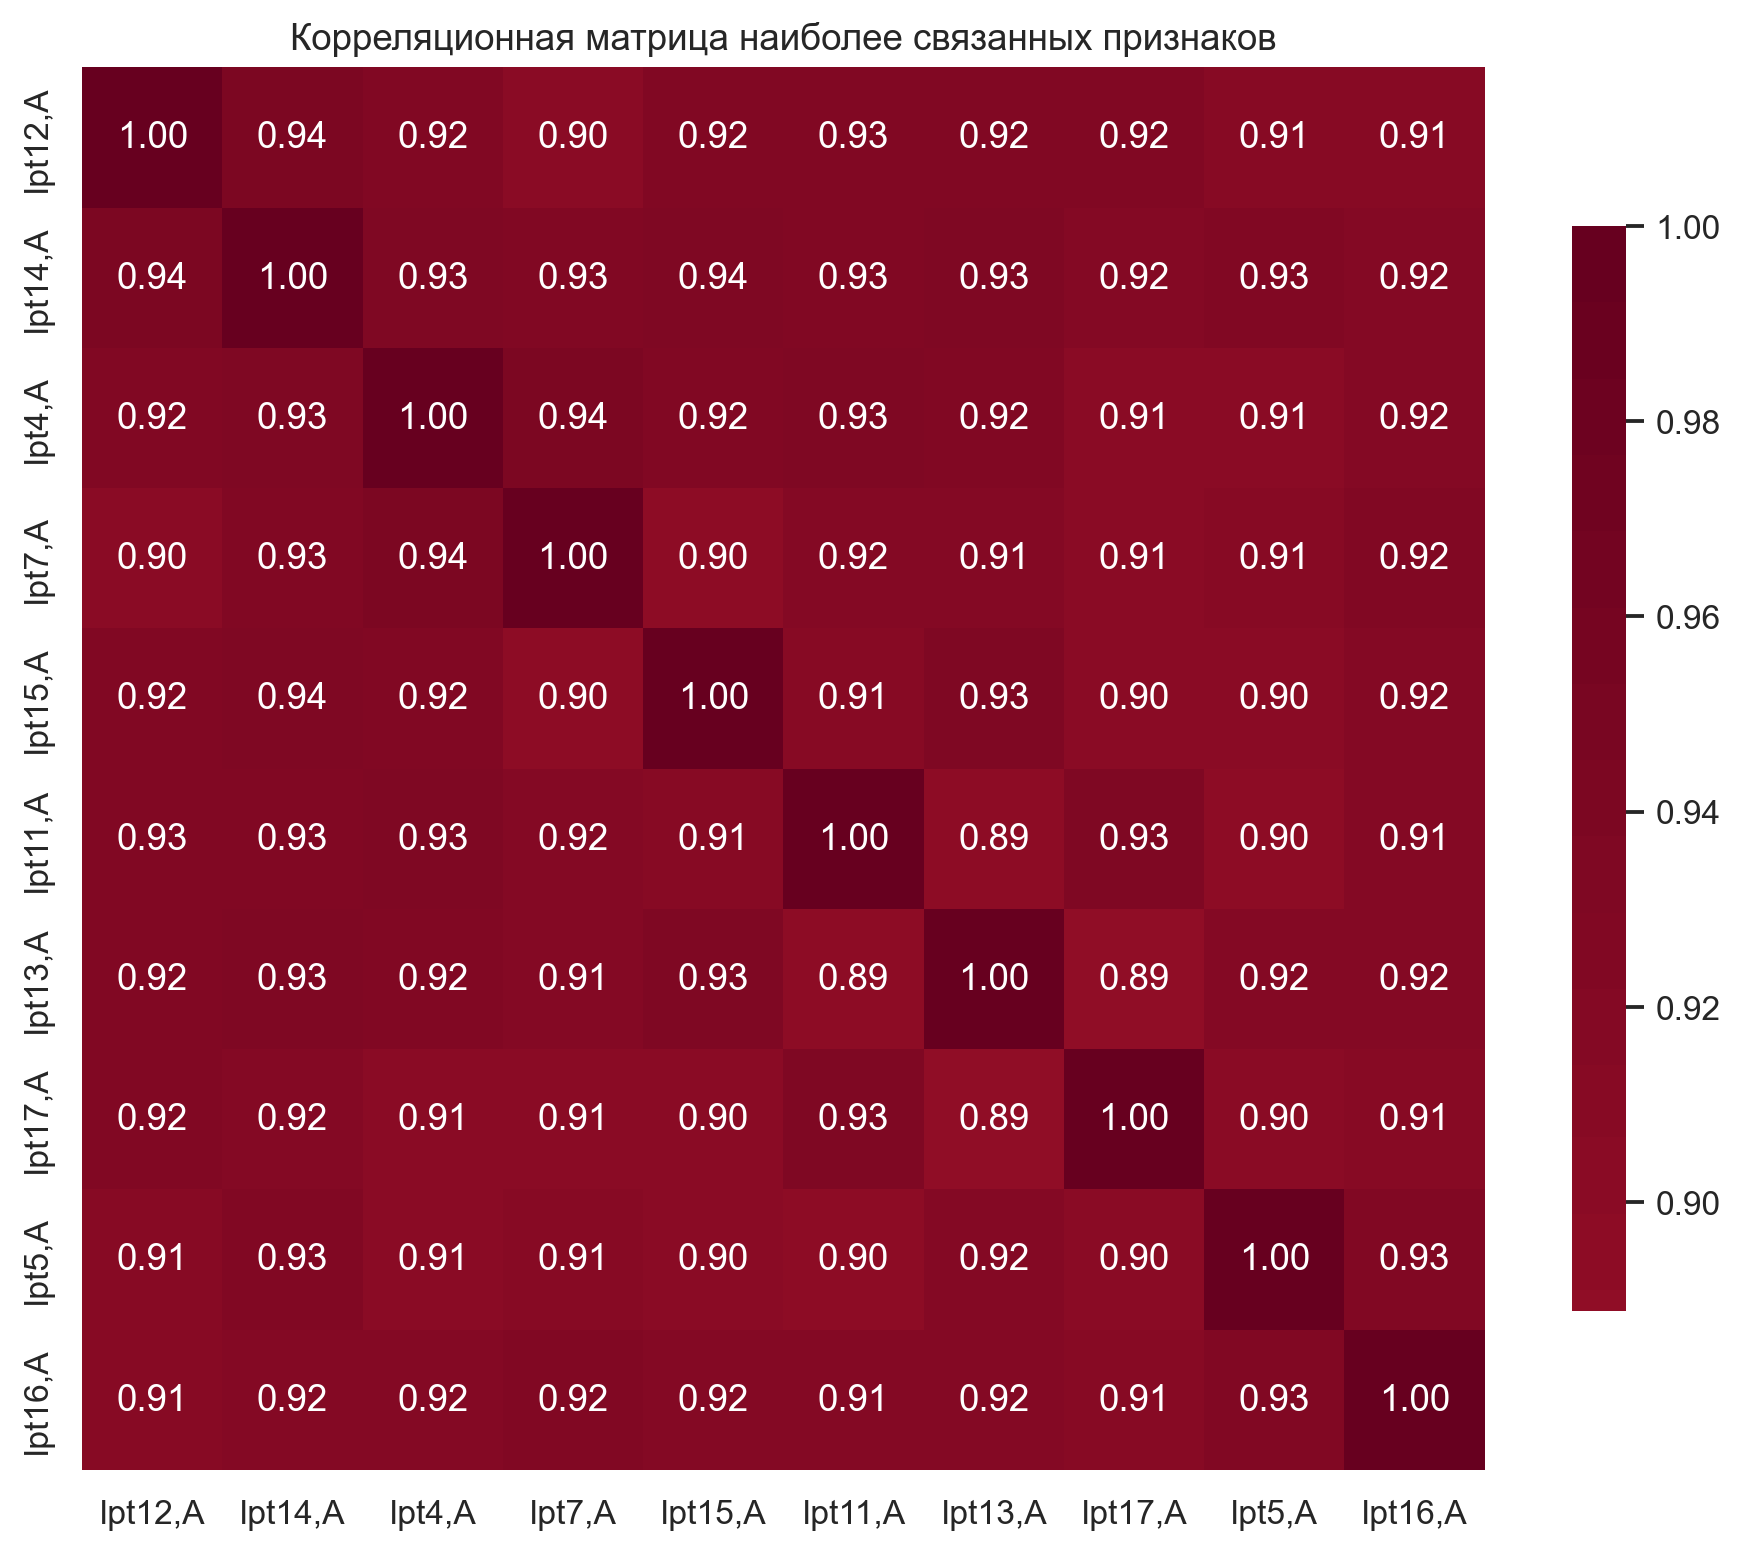
\includegraphics[width=0.92\textwidth]{correlation_heatmap.png}
\caption{Корреляционная структура признакового пространства}
\end{figure}

\section{Подготовка данных и аугментация}\label{sec:prep}
Были реализованы две версии подготовки признаков.

\subsection{Базовая версия raw}
Для варианта \texttt{raw} выполняется только median-импутация по статистикам обучающей части. Такой вариант используется как контрольный, поскольку он минимально изменяет исходные ряды.

\subsection{Улучшенная версия improved}
Вариант \texttt{improved} включает три последовательных операции:
\begin{enumerate}
    \item median-импутацию по обучающей части;
    \item winsorization по квантильным границам $q_{0.01}$ и $q_{0.99}$;
    \item робастное масштабирование (\texttt{RobustScaler}) по медиане и межквартильному размаху.
\end{enumerate}

Пусть $x$ --- исходное значение признака, тогда ограничение по квантилям записывается как
\begin{equation}
    \tilde{x}=\min\{\max\{x, q_{0.01}\}, q_{0.99}\}.
\end{equation}
После этого выполняется робастная нормализация:
\begin{equation}
    x^{*}=\frac{\tilde{x}-\mathrm{median}(x)}{\mathrm{IQR}(x)}.
\end{equation}

\subsection{Аугментация временных окон}\label{sec:augmentation}
Для снижения вариативности результатов и повышения устойчивости обучения в проект добавлена аугментация окон. Она применяется только к обучающей части и не затрагивает \texttt{validation} и \texttt{test}. Реализованы три метода:
\begin{enumerate}
    \item добавление гауссовского шума;
    \item случайное масштабирование амплитуды;
    \item циклический временной сдвиг окна.
\end{enumerate}

Если $X$ обозначает окно, а $\varepsilon \sim \mathcal{N}(0,\sigma^2)$ --- шум такой же размерности, то шумовая аугментация задаётся выражением:
\begin{equation}
    X_{\mathrm{noise}} = X + \varepsilon.
\end{equation}
Амплитудное масштабирование реализуется как
\begin{equation}
    X_{\mathrm{scale}} = \alpha X, \qquad \alpha \in [0.9, 1.1],
\end{equation}
а временной сдвиг --- как перестановка по оси времени на $\Delta t$ шагов. В текущей конфигурации коэффициент расширения выборки равен трём, поэтому число обучающих окон увеличивается с 55 до 165.

\begin{figure}[H]
\centering
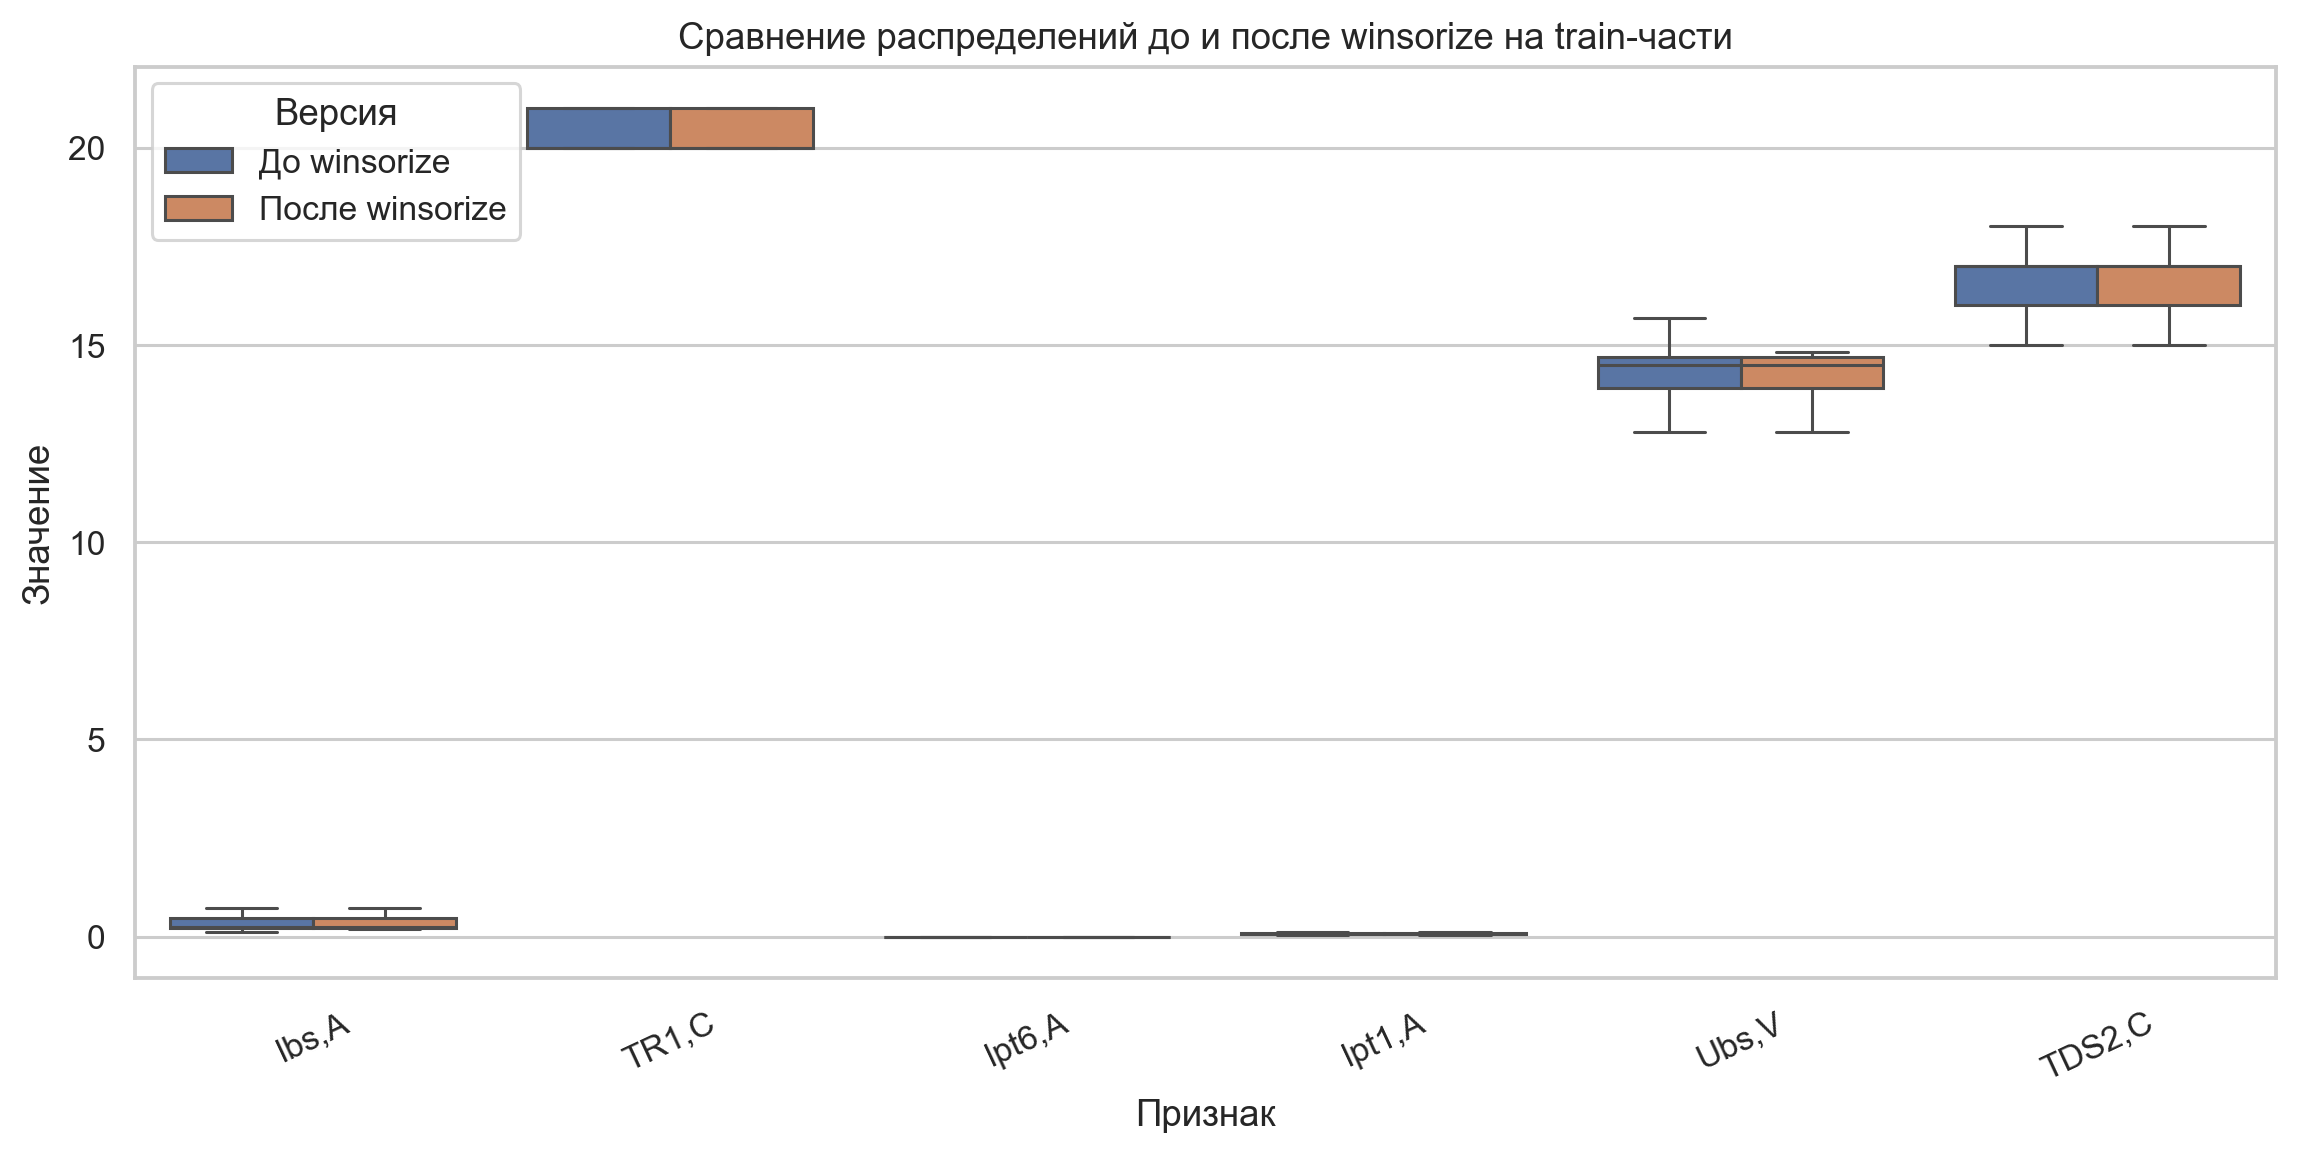
\includegraphics[width=0.85\textwidth]{winsorization_boxplots.png}
\caption{Эффект winsorization и робастного масштабирования на распределения признаков}
\end{figure}

\section{Метрики качества и ROC AUC-анализ}\label{sec:metrics}
В качестве основных критериев оценки выбраны \textit{macro-F1}, \textit{balanced accuracy} и \textit{ROC AUC} в постановке One-vs-Rest с макроусреднением.

Macro-F1 определяется как среднее арифметическое F1-оценок по классам:
\begin{equation}
    F1_{macro}=\frac{1}{K}\sum_{k=1}^{K} F1_k,
\end{equation}
где
\begin{equation}
    F1_k = \frac{2 P_k R_k}{P_k + R_k}, \qquad
    P_k = \frac{TP_k}{TP_k + FP_k}, \qquad
    R_k = \frac{TP_k}{TP_k + FN_k}.
\end{equation}

Balanced accuracy используется для компенсации дисбаланса классов и вычисляется как средняя полнота:
\begin{equation}
    BA = \frac{1}{K}\sum_{k=1}^{K} \frac{TP_k}{TP_k + FN_k}.
\end{equation}

ROC AUC рассчитывается в схеме One-vs-Rest. Для каждого класса строится бинарная кривая ROC, а затем площади под кривыми усредняются:
\begin{equation}
    AUC_{macro}^{OvR} = \frac{1}{K'}\sum_{k \in \mathcal{C}_{present}} AUC_k,
\end{equation}
где $\mathcal{C}_{present}$ --- множество классов, реально присутствующих в \texttt{y\_true} текущего разбиения, а $K'=|\mathcal{C}_{present}|$. Такое определение было внедрено в обновлённую версию проекта, поскольку при временном разбиении некоторые редкие классы могут отсутствовать в конкретной валидационной части.

Интерпретация ROC AUC следующая:
\begin{itemize}
    \item $AUC \approx 0.5$ соответствует уровню случайного угадывания;
    \item $AUC > 0.7$ означает приемлемую разделимость;
    \item $AUC > 0.8$ указывает на хорошую разделимость;
    \item $AUC > 0.9$ соответствует очень высокой способности модели ранжировать положительные и отрицательные случаи;
    \item $AUC = 1.0$ означает идеальное ранжирование на текущем наборе примеров.
\end{itemize}

Важно, что при текущем официальном \texttt{validation}-срезе отсутствует класс 1, поэтому ROC AUC вычисляется только по классам 0 и 2. В отчёте это всегда явно помечается отдельным примечанием, а интерпретация не распространяется на отсутствующий класс.

\section{Базовые модели и диагностический анализ обучения}\label{sec:baseline}
В качестве базовой модели использовалась \texttt{LogisticRegression} с балансировкой классов. Она обучалась на векторизованных временных окнах размерности $128\times49=6272$ признака на одно окно. Несмотря на простоту, baseline позволяет задать минимальный уровень качества, относительно которого оценивается выигрыш нейросетевых архитектур.

На \texttt{raw}-данных baseline показал $macro\text{-}F1=0.1818$, $BA=0.1875$, $ROC\ AUC=0.5625$. На версии \texttt{improved} результат вырос до $macro\text{-}F1=0.3137$, однако $ROC\ AUC$ снизился до $0.1875$, что указывает на слабую ранжирующую способность логистической модели на текущем временном срезе. С точки зрения практической эксплуатации baseline остаётся полезным как быстрая и интерпретируемая контрольная модель, но не как основной классификатор.

Поскольку в используемом API логистическая регрессия не предоставляет удобной покадровой истории loss, comparable с нейросетевыми эпохами, для baseline основными диагностическими материалами выступают ROC-кривые и анализ коэффициентов модели.

\begin{figure}[H]
\centering
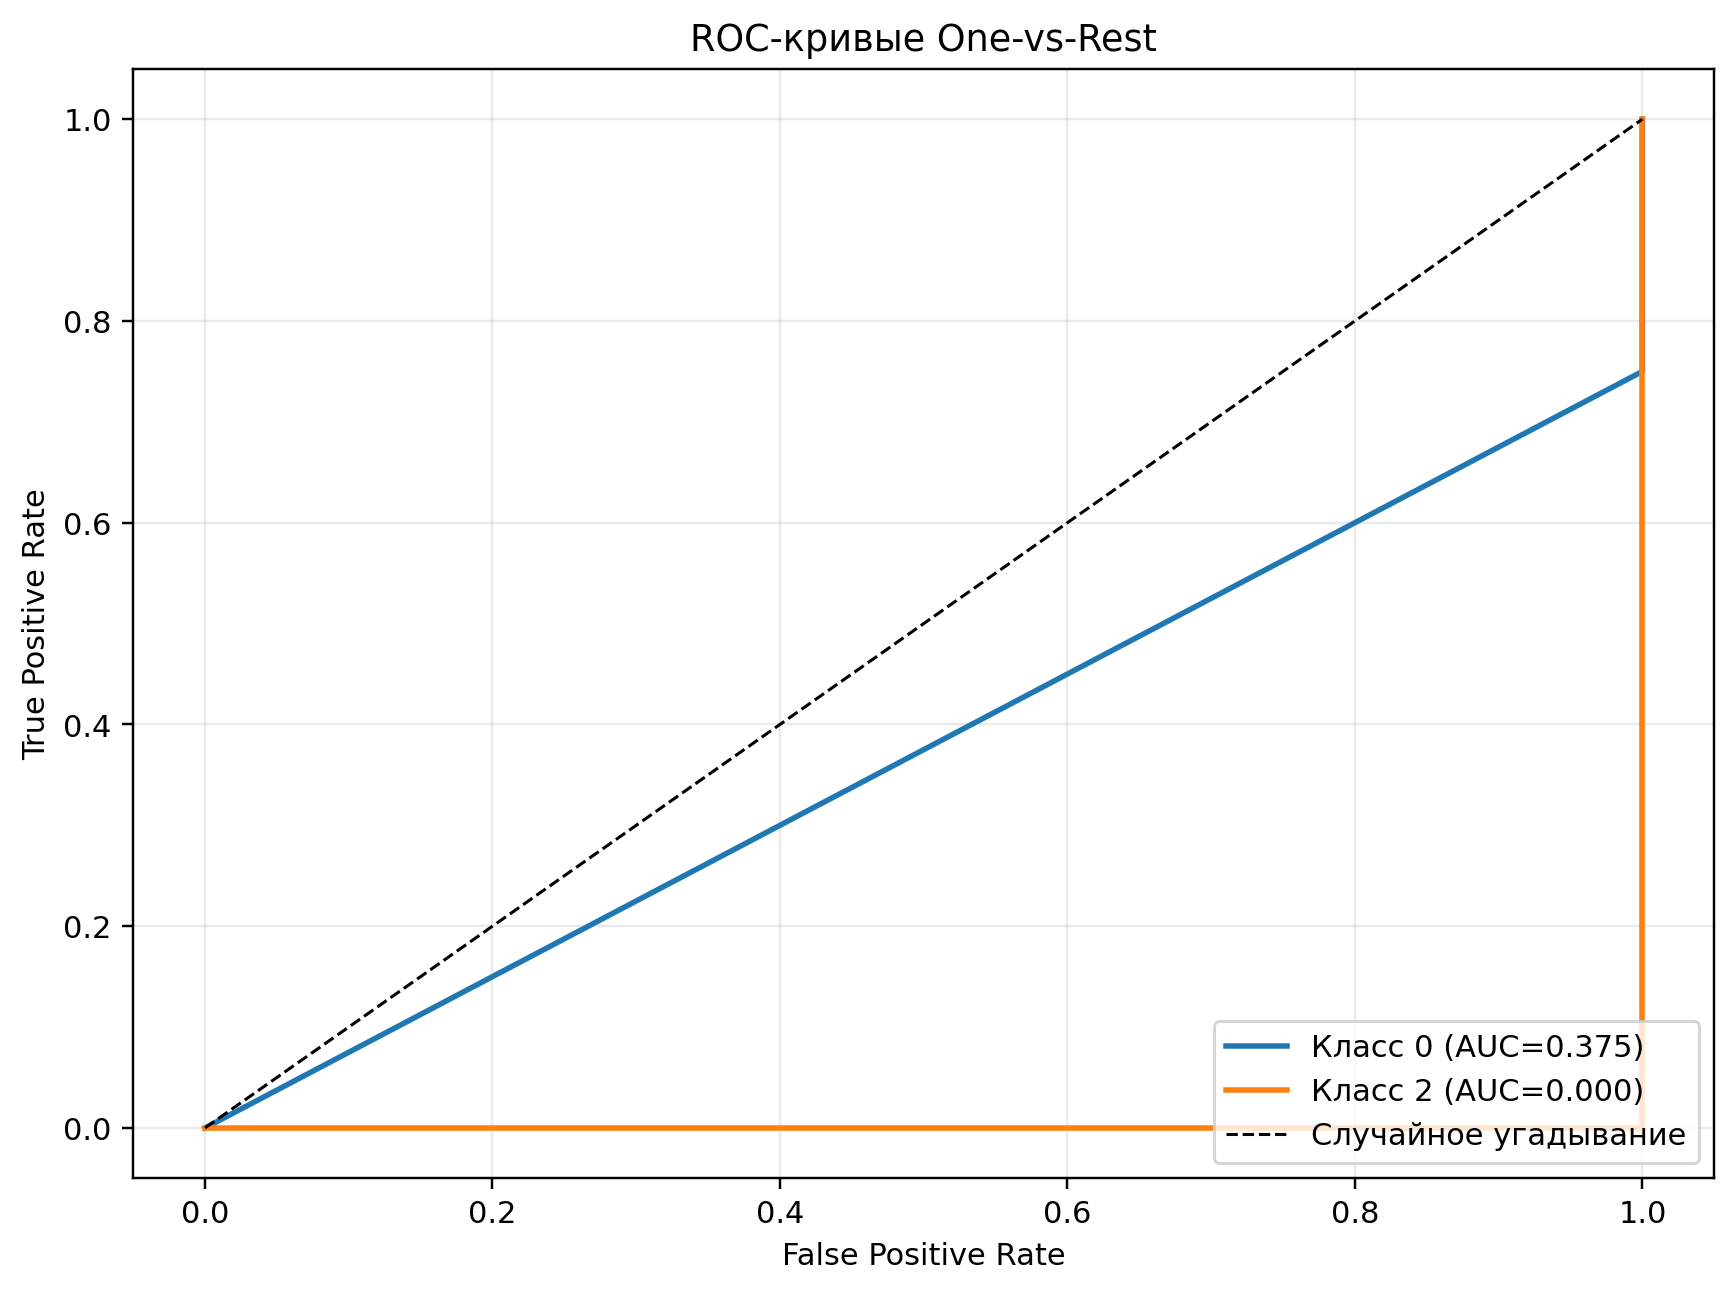
\includegraphics[width=0.72\textwidth]{stage4_baseline_improved_roc.png}
\caption{ROC-кривые baseline-модели для версии данных improved}
\end{figure}

\begin{figure}[H]
\centering
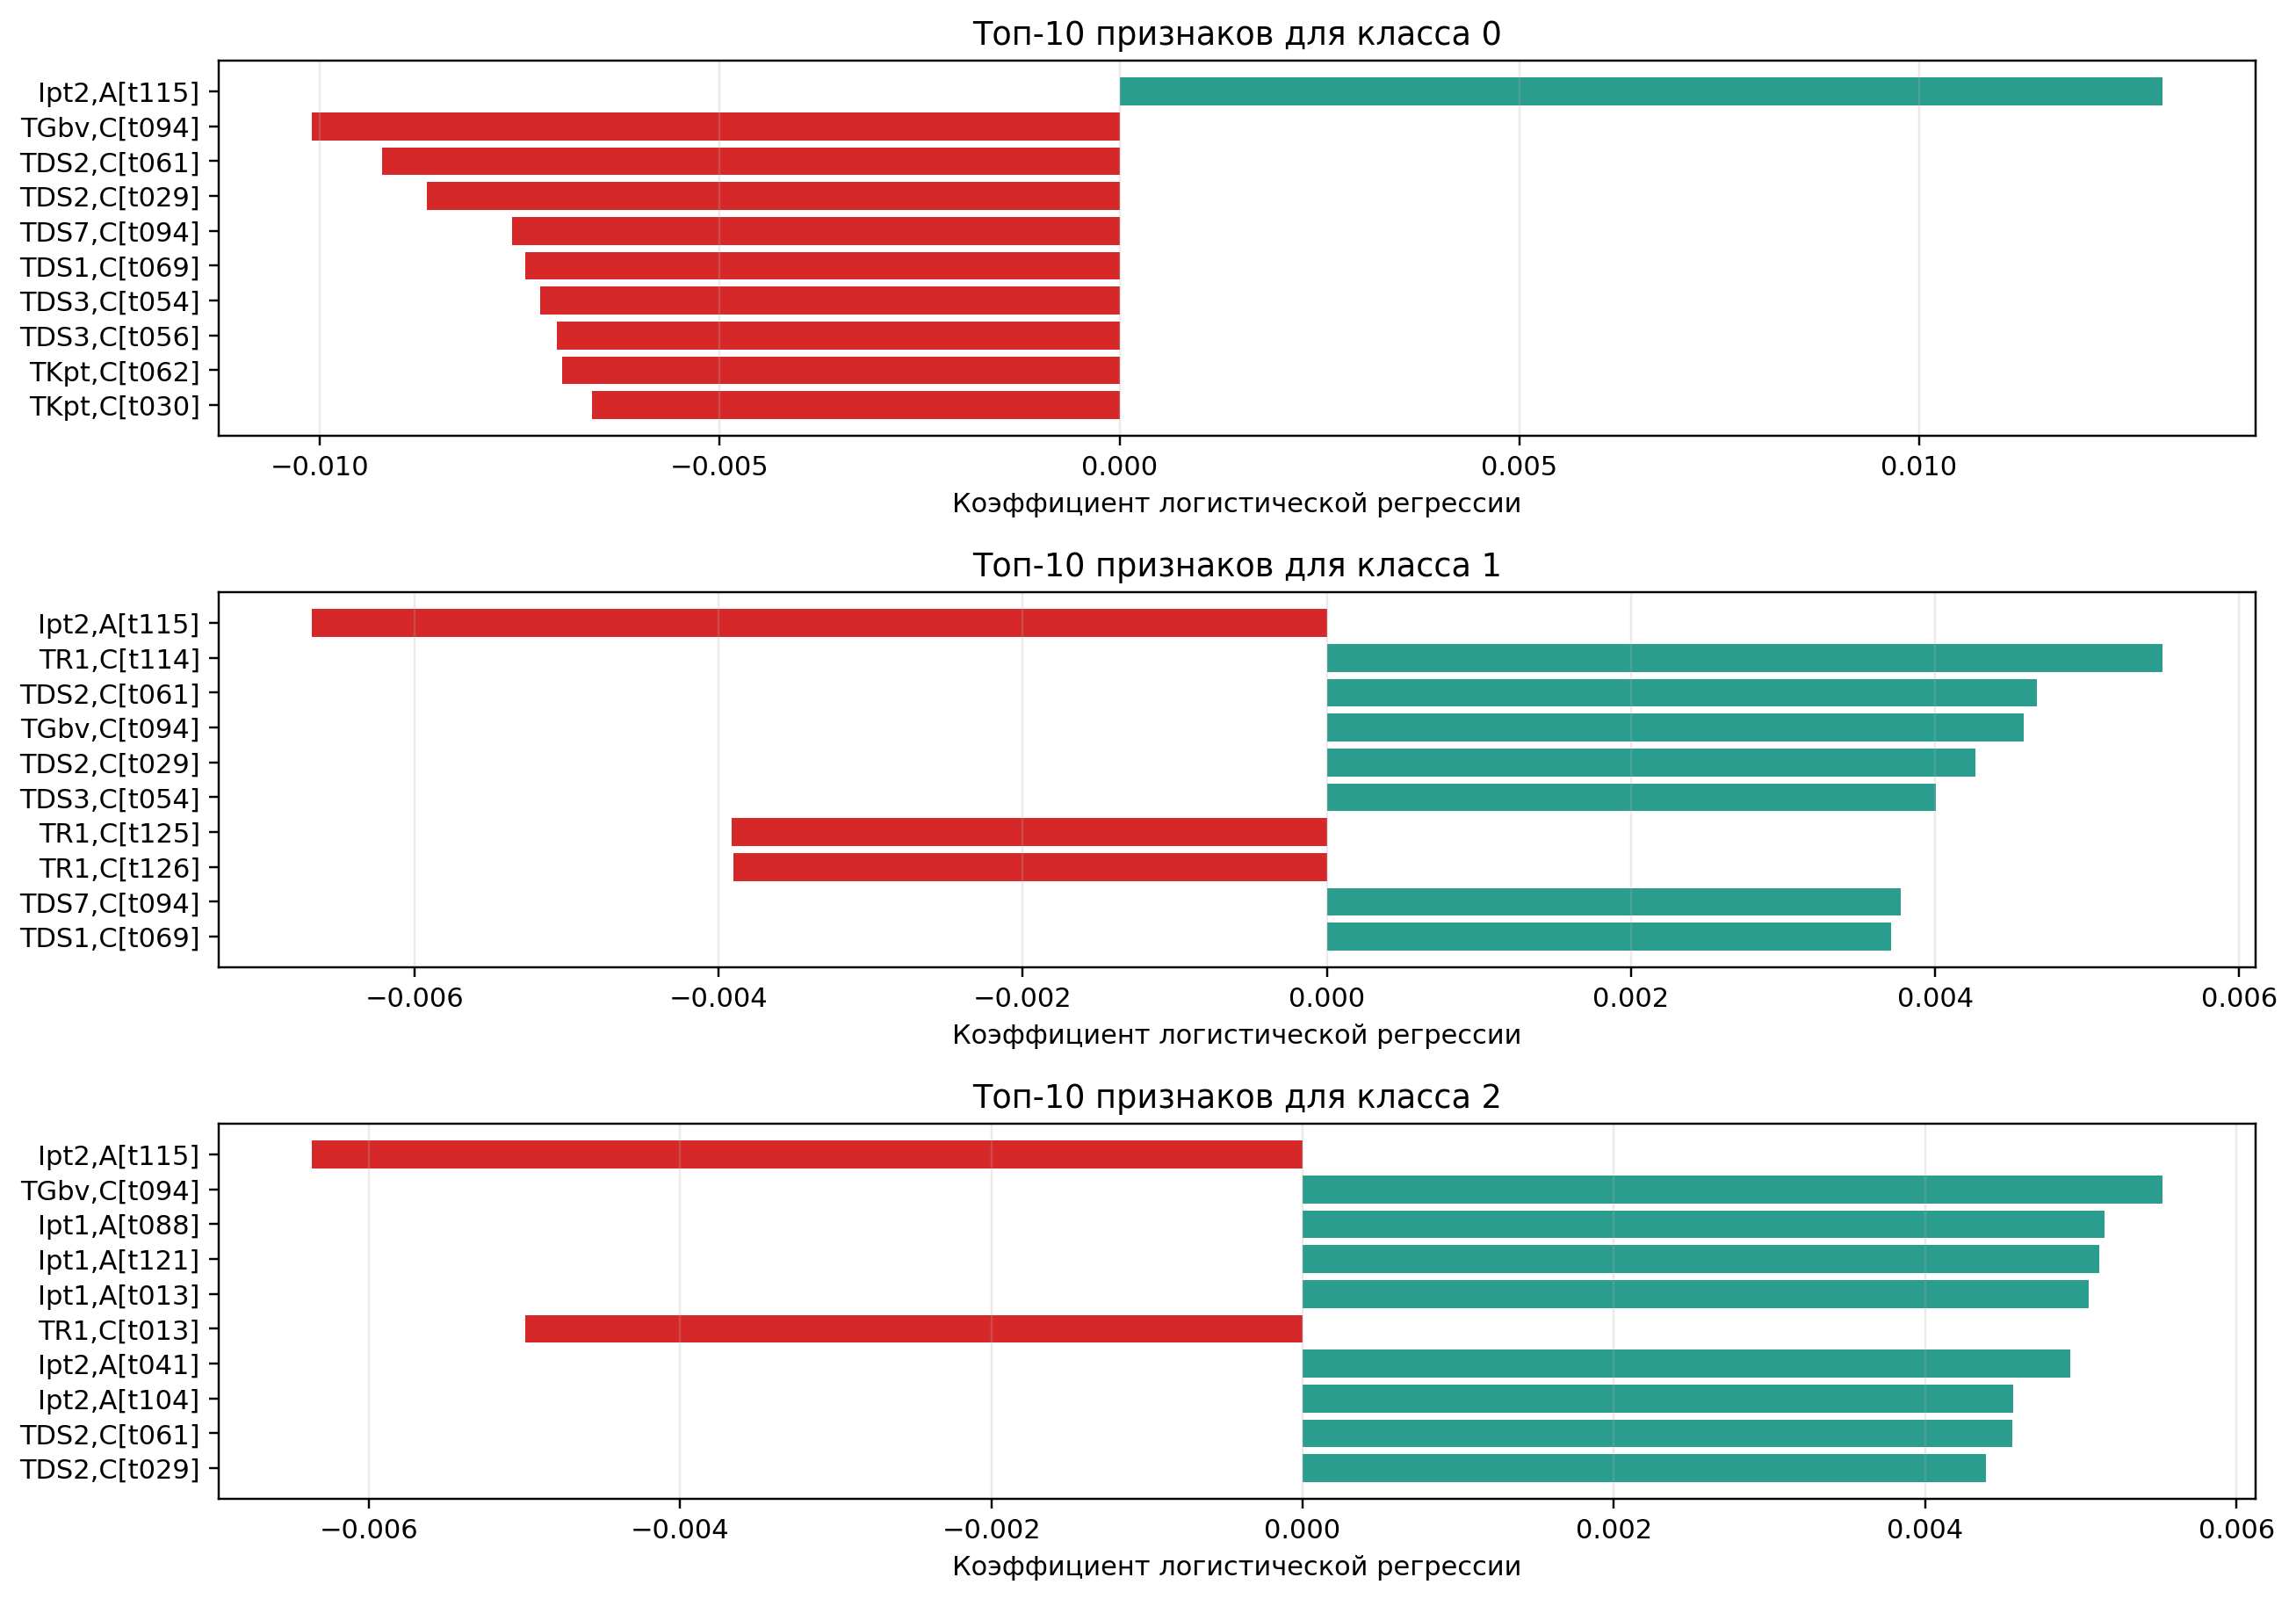
\includegraphics[width=0.9\textwidth]{stage4_baseline_improved_feature_importance.png}
\caption{Топ признаков по модулю коэффициентов логистической регрессии}
\end{figure}

Коэффициенты baseline показывают, что наиболее значимые признаки сконцентрированы в нескольких температурных, токовых и напряженческих каналах. Это согласуется с инженерной логикой: при переходе в нештатное состояние именно физические параметры питания, теплового режима и нагрузок изменяются раньше всего.

\section{Гибридная нейросетевая архитектура и диагностика обучения}\label{sec:hybrid}
Основная модель проекта представляет собой каскад \texttt{1D-CNN \textrightarrow RNN \textrightarrow Dense}. Сверточный блок выделяет локальные временные паттерны в пределах окна, рекуррентный блок аккумулирует контекст по времени, а полносвязная часть формирует итоговое распределение вероятностей по трём классам.

\begin{figure}[H]
\centering

\includegraphics[width=0.88\textwidth]{hybrid_scheme.png}
\caption{Структурная схема гибридной модели временной классификации}
\end{figure}

При обучении использовались \texttt{EarlyStopping} и \texttt{ReduceLROnPlateau}, а также весовые коэффициенты классов по формуле balanced:
\begin{equation}
    w_k = \frac{N}{K \cdot n_k},
\end{equation}
где $N$ --- объём обучающего набора, $K$ --- число присутствующих классов в train, $n_k$ --- число примеров класса $k$.

\subsection{Диагностика обучения}\label{sec:train_diagnostics}
В рамках улучшения проекта история обучения сохраняется в виде JSON и визуализируется графиками loss и accuracy. Это позволяет диагностировать начало переобучения и подтверждать корректность выбора лучшей эпохи по \texttt{validation loss}.

Для \texttt{improved}-версии базовой GRU-модели лучшей оказалась 10-я эпоха при общем числе 15 выполненных эпох. Кривые показывают, что после достижения минимума валидационной ошибки дальнейшее уменьшение train-loss уже не приводит к устойчивому улучшению качества на \texttt{validation}. Следовательно, механизм ранней остановки в текущем проекте настроен корректно и реально ограничивает переобучение.

\begin{figure}[H]
\centering
\includegraphics[width=0.9\textwidth]{training_curves.png}
\caption{Графики обучения гибридной модели (improved, базовый GRU-вариант)}
\end{figure}

На \texttt{raw}-данных гибридная модель дала $macro\text{-}F1=0.3111$, а на \texttt{improved}-данных --- $macro\text{-}F1=0.6444$, $BA=0.9375$, $ROC\ AUC=1.0$ по присутствующим классам. Таким образом, улучшенная предобработка даёт принципиальный выигрыш и должна рассматриваться как стандартный путь подготовки данных для дальнейших экспериментов.

\begin{figure}[H]
\centering
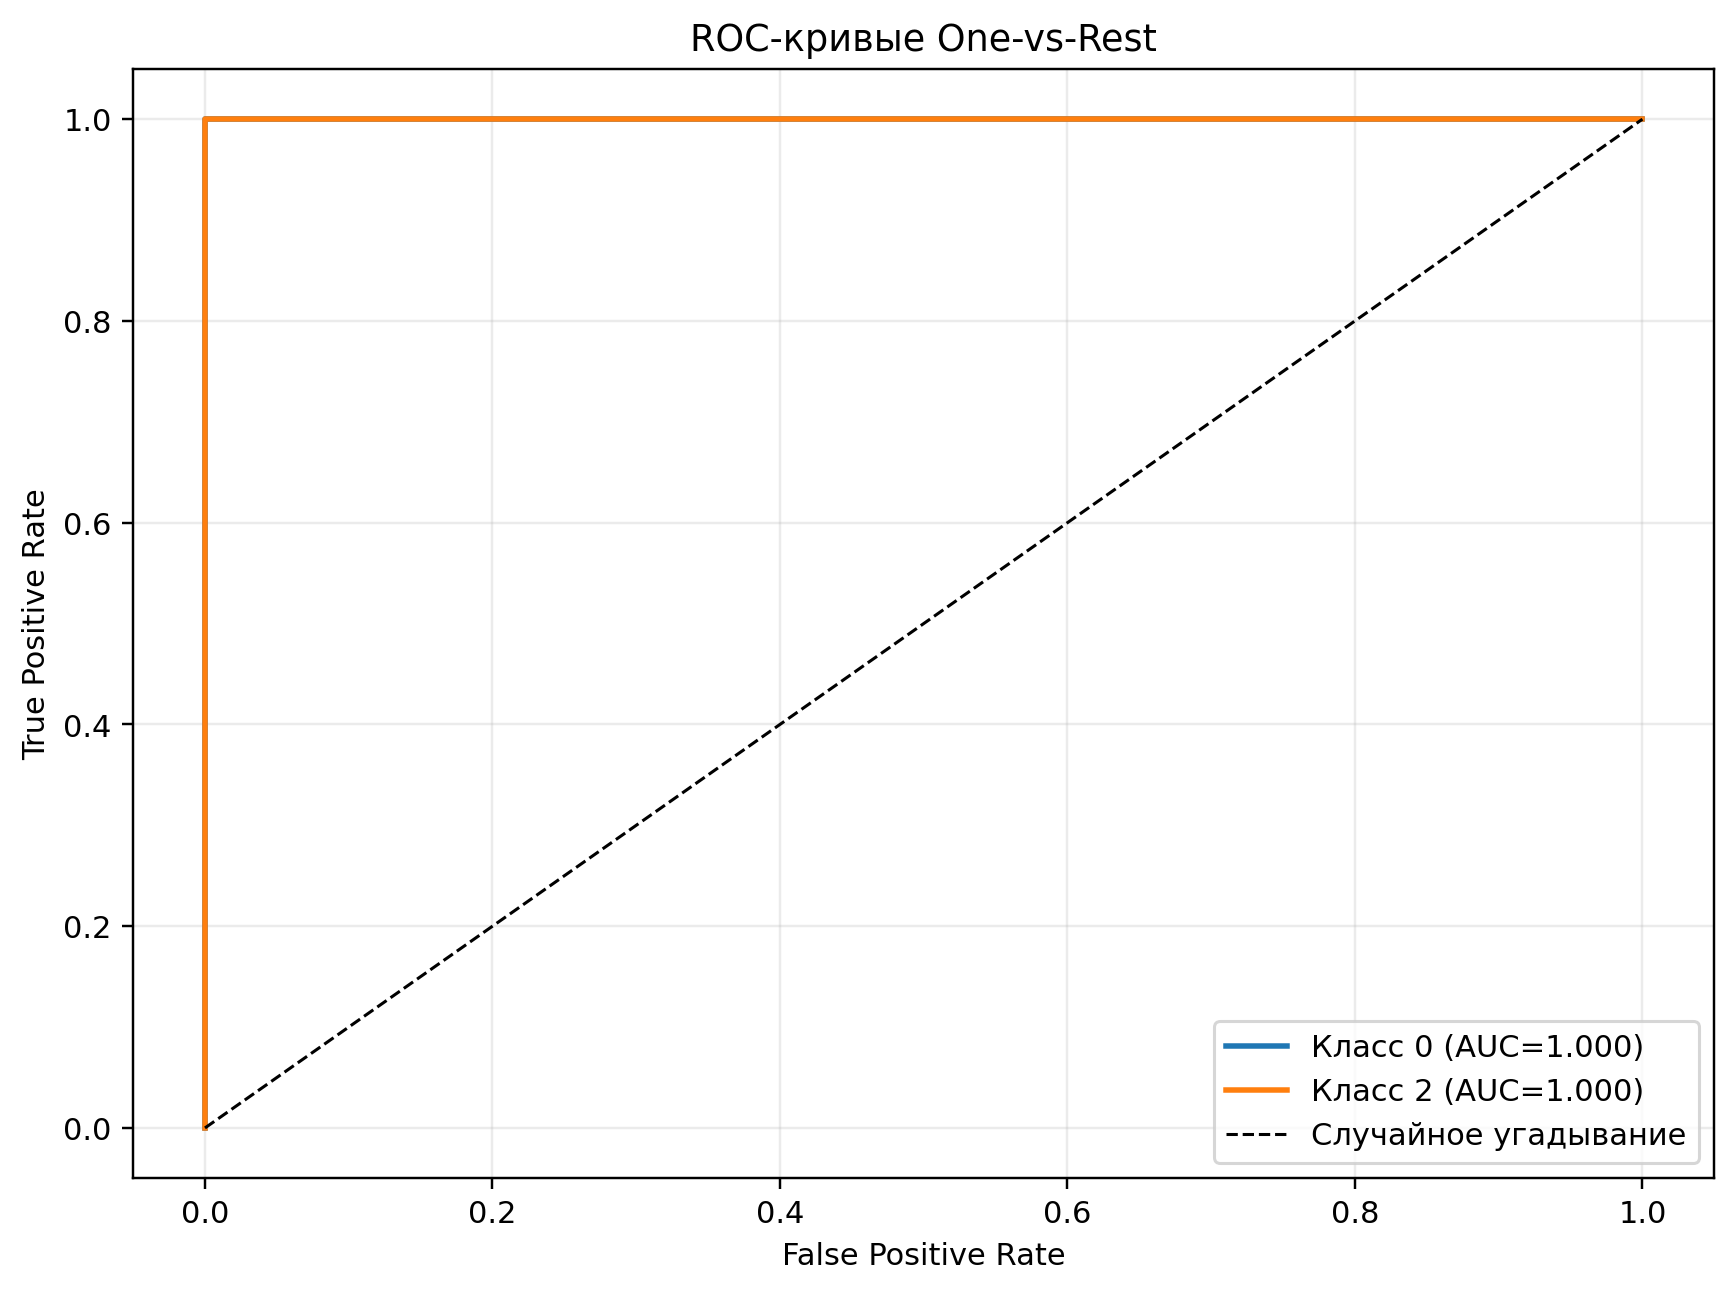
\includegraphics[width=0.72\textwidth]{stage5_improved_roc.png}
\caption{ROC-кривые базовой гибридной модели для improved-набора}
\end{figure}

\section{Сравнение рекуррентных блоков и исследование attention}\label{sec:rnn}
\subsection{Сравнение типов рекуррентного слоя}\label{sec:rnn_choice}
Для экспериментального обоснования выбора рекуррентного блока были реализованы четыре варианта: \texttt{GRU}, \texttt{LSTM}, \texttt{Bi-GRU}, \texttt{Bi-LSTM}. Результаты сравнения приведены в таблице~\ref{tab:rnn_compare}.

\begin{table}[H]
\centering
\caption{Сравнение рекуррентных блоков на improved-данных}
\label{tab:rnn_compare}
\begin{tabular}{>{\raggedright\arraybackslash}p{0.18\textwidth}cccc}
\toprule
Тип RNN & Параметры & macro-F1 & BA & ROC AUC \\
\midrule
GRU & 107395 & 0.6444 & 0.9375 & 1.0000 \\
LSTM & 131715 & 0.6444 & 0.9375 & 1.0000 \\
Bi-GRU & 198275 & 0.6667 & 1.0000 & 1.0000 \\
Bi-LSTM & 246915 & 0.6667 & 1.0000 & 1.0000 \\
\bottomrule
\end{tabular}
\end{table}

С инженерной точки зрения выбор \texttt{GRU} остаётся оправданным как базовый компромисс между числом параметров и качеством: по сравнению с \texttt{LSTM} он обеспечивает то же качество при меньшей сложности. Двунаправленные варианты действительно улучшают метрики на текущем \texttt{validation}, но такой выигрыш достигается почти двукратным ростом числа параметров. Для эксплуатационного контура, где важны вычислительная стоимость и устойчивость, этот компромисс должен приниматься осознанно.

\subsection{Сравнение без attention и с attention}\label{sec:attention}
В архитектуру был добавлен отдельный слой внимания, который формирует веса для временных шагов и агрегирует контекстную последовательность в один вектор признаков:
\begin{equation}
    e_t = v^\top \tanh(W h_t), \qquad
    \alpha_t = \frac{\exp(e_t)}{\sum_j \exp(e_j)}, \qquad
    c = \sum_t \alpha_t h_t.
\end{equation}

На текущем срезе \texttt{validation} добавление внимания не улучшило качество, а, наоборот, ухудшило его: $macro\text{-}F1$ снизился до $0.3137$, а $ROC\ AUC$ для присутствующих классов опустился до $0.0$. Это означает, что при столь малом числе валидационных окон attention-подсистема оказалась переусложнением и не смогла устойчиво научиться полезному распределению фокуса.

\begin{figure}[H]
\centering
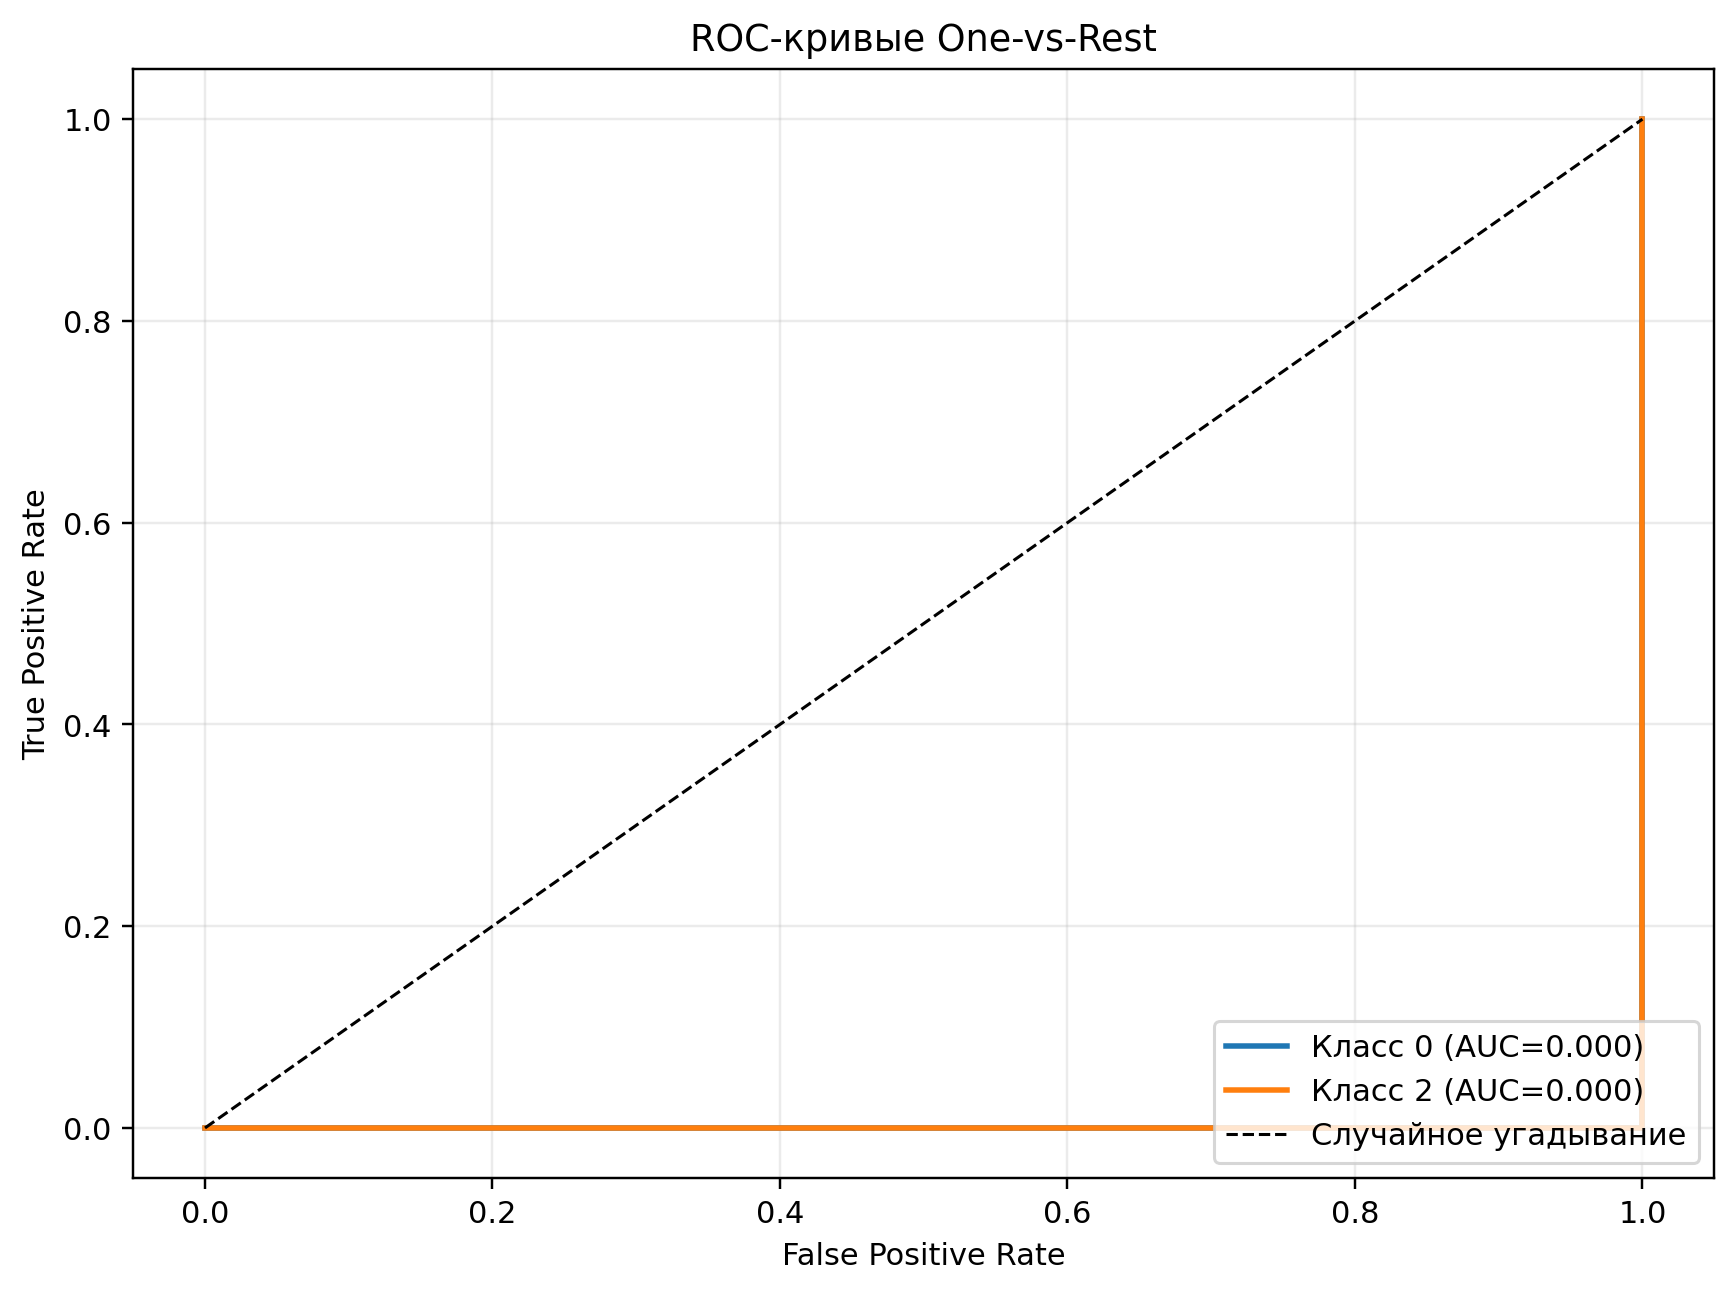
\includegraphics[width=0.72\textwidth]{stage5_attention_roc.png}
\caption{ROC-кривые модели с attention; видно ухудшение ранжирования}
\end{figure}

\begin{figure}[H]
\centering
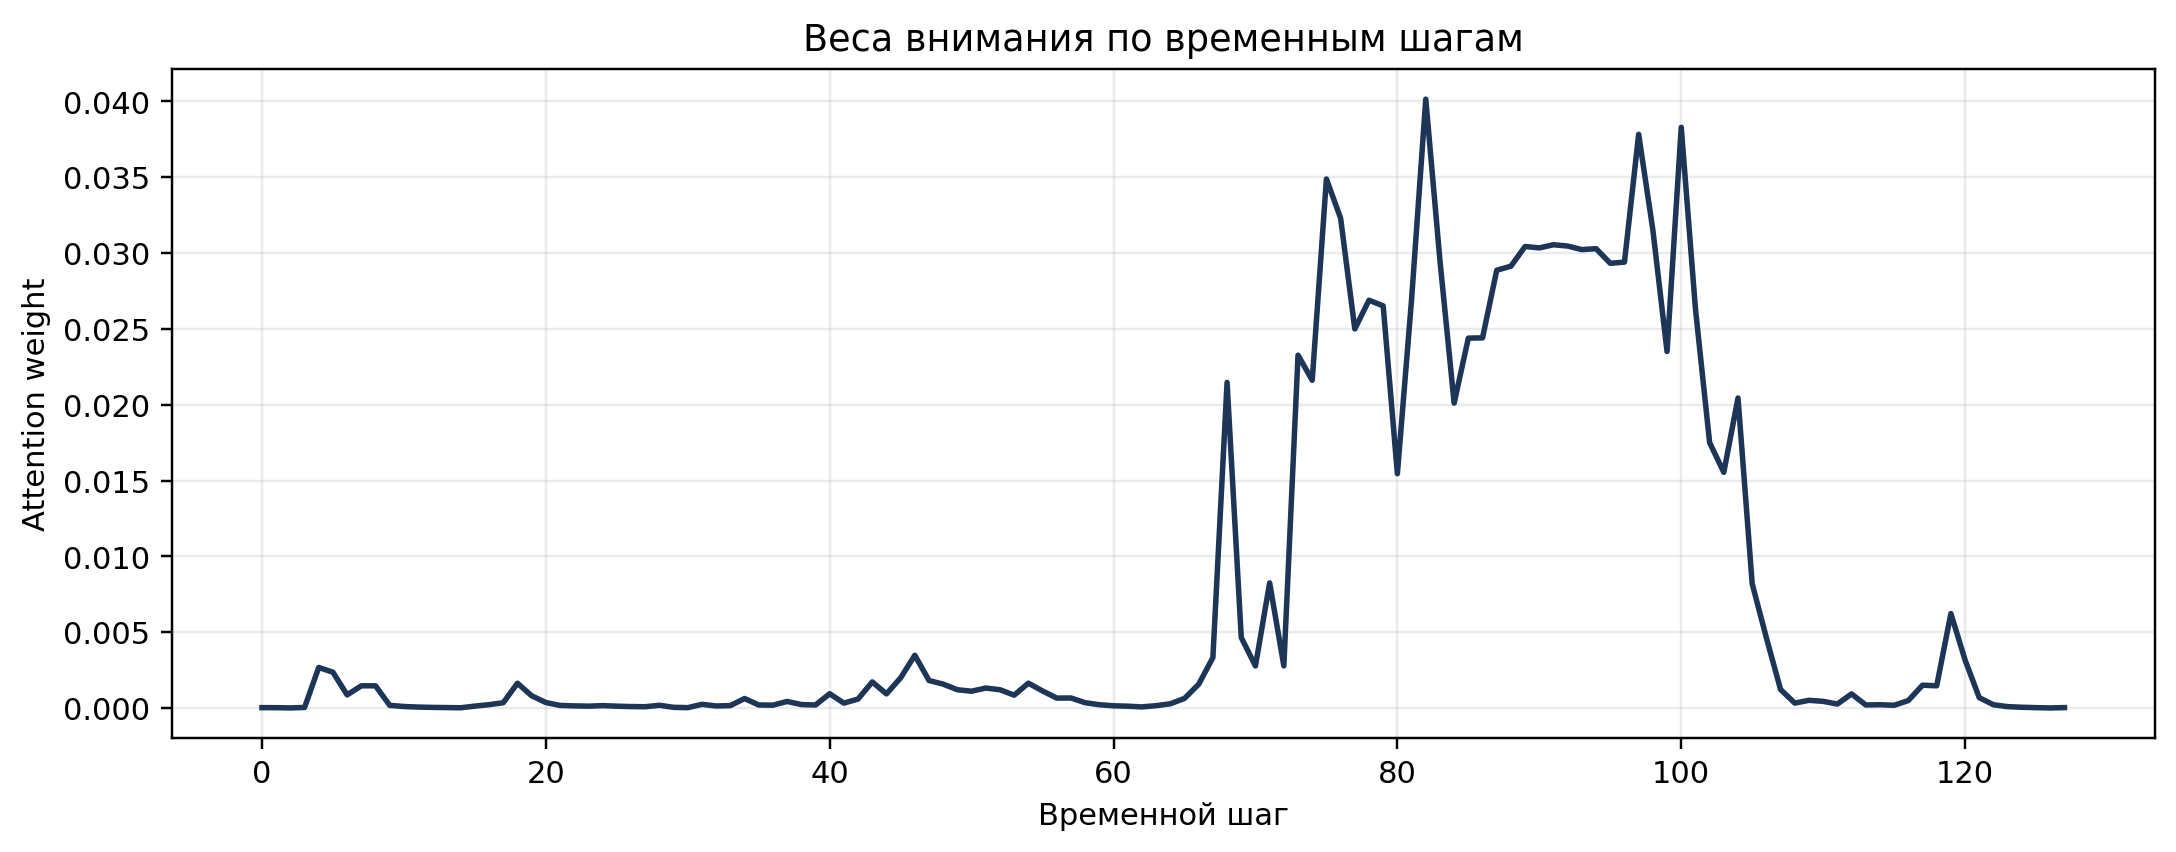
\includegraphics[width=0.88\textwidth]{stage5_attention_weights.png}
\caption{Пример распределения attention-весов по временным шагам}
\end{figure}

\section{Оптимизация и предобучение}\label{sec:optimization}
\subsection{Генетический поиск гиперпараметров}
Генетический алгоритм использовался для поиска конфигурации по девяти гиперпараметрам: числу сверточных и рекуррентных слоёв, размеру фильтров, размеру ядра, числу dense-слоёв, размеру dense-блока, типу оптимизатора и функции активации. В качестве fitness использовался \texttt{macro-F1} на официальном \texttt{validation} без вовлечения дополнительной rolling-диагностики в критерий отбора.

Постфактум-диагностика сохранённой лучшей модели этапа 6 показала: $macro\text{-}F1=0.6667$, $BA=1.0000$, $ROC\ AUC=1.0000$ по присутствующим классам 0 и 2. Тем самым GA-конфигурация превзошла как baseline, так и базовый GRU-вариант.

\begin{figure}[H]
\centering

\includegraphics[width=0.84\textwidth]{ga_progress.png}
\caption{Динамика GA-поиска по поколениям}
\end{figure}

\begin{figure}[H]
\centering
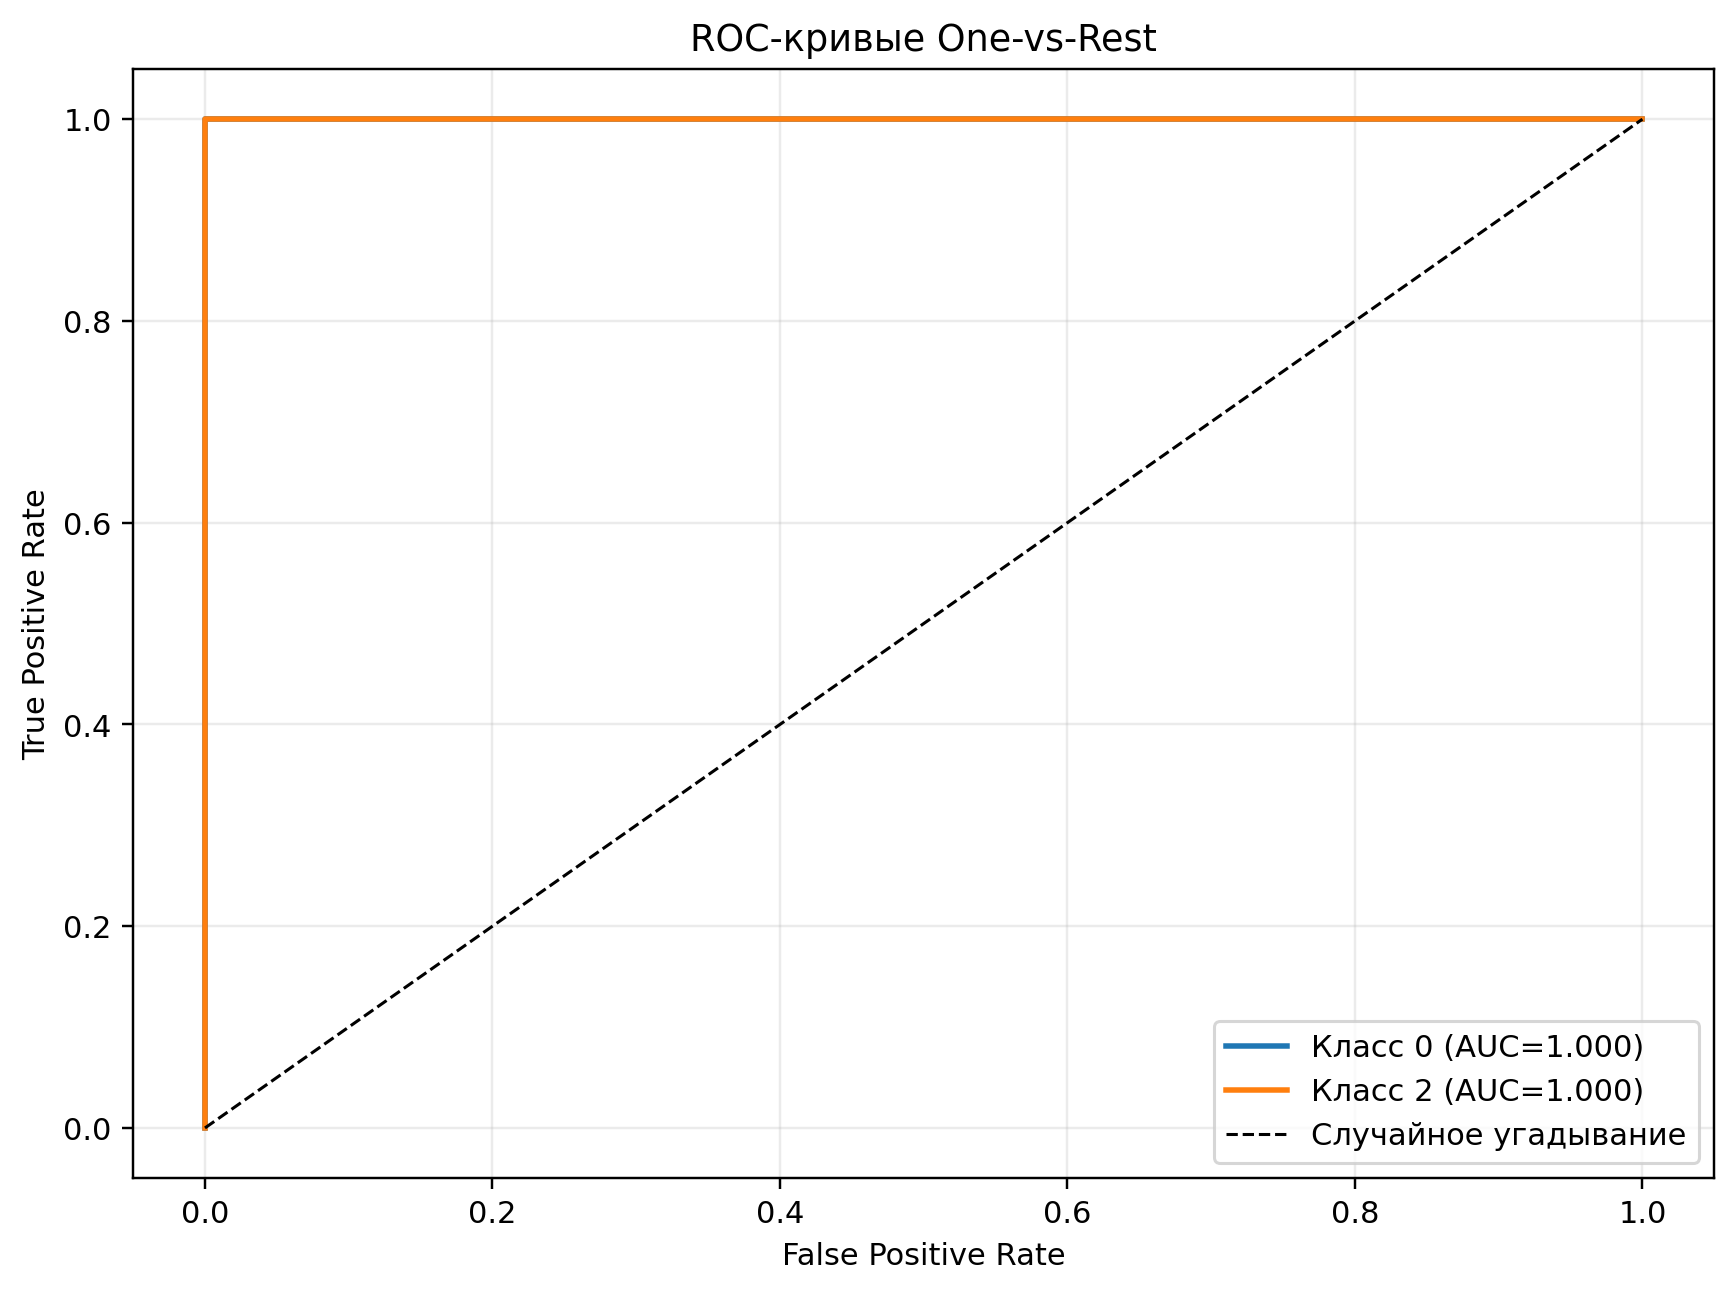
\includegraphics[width=0.72\textwidth]{stage6_ga_best_val_roc.png}
\caption{ROC-кривые лучшей GA-модели на validation}
\end{figure}

\subsection{Предобучение автоэнкодера}
Для использования неразмеченной телеметрии реализован автоэнкодер, в котором encoder-подсистема повторяет сверточно-рекуррентную часть классификатора, а decoder восстанавливает исходное окно. Такая схема позволяет дообучать encoder на задаче реконструкции и затем переносить веса в классификатор.

\begin{figure}[H]
\centering

\includegraphics[width=0.88\textwidth]{autoencoder_scheme.png}
\caption{Схема автоэнкодера для реконструкционного предобучения}
\end{figure}

На текущем наборе данных предобучение автоэнкодера не дало прироста качества по сравнению с обучением классификатора с нуля: для обеих версий получено $macro\text{-}F1=0.6444$, а постфактум-ROC AUC составил $0.9375$. Это важный исследовательский результат: сам по себе факт наличия неразмеченной выборки ещё не гарантирует выигрыша, если downstream-задача уже хорошо решается базовым supervised-контуром и размер fine-tuning-выборки невелик.

\section{Интерпретация модели}\label{sec:interpretation}
\subsection{Важность признаков baseline-модели}
Коэффициенты логистической регрессии позволяют выделить группы признаков, которые сильнее всего влияют на решение по каждому классу. Положительные коэффициенты означают рост логита для рассматриваемого класса при увеличении значения признака, отрицательные --- обратный эффект. Несмотря на линейность модели, этот анализ полезен как первичная инженерная интерпретация.

В текущем проекте максимальный вклад в решение baseline вносят временные фрагменты токовых и температурных каналов. Это физически правдоподобно: отклонения токов и тепловых параметров отражают как отказ силовых трактов, так и деградацию подсистемы питания.

\subsection{Визуализация свёрточных фильтров и скрытых представлений}\label{sec:conv_interp}
Для гибридной модели дополнительно построены две визуализации: карта весов первого сверточного слоя и двумерная проекция скрытых представлений последнего рекуррентного блока. Первая позволяет понять, какие комбинации каналов и коротких временных шаблонов ищет модель, а вторая --- увидеть, насколько хорошо классы разделяются в латентном пространстве.

\begin{figure}[H]
\centering
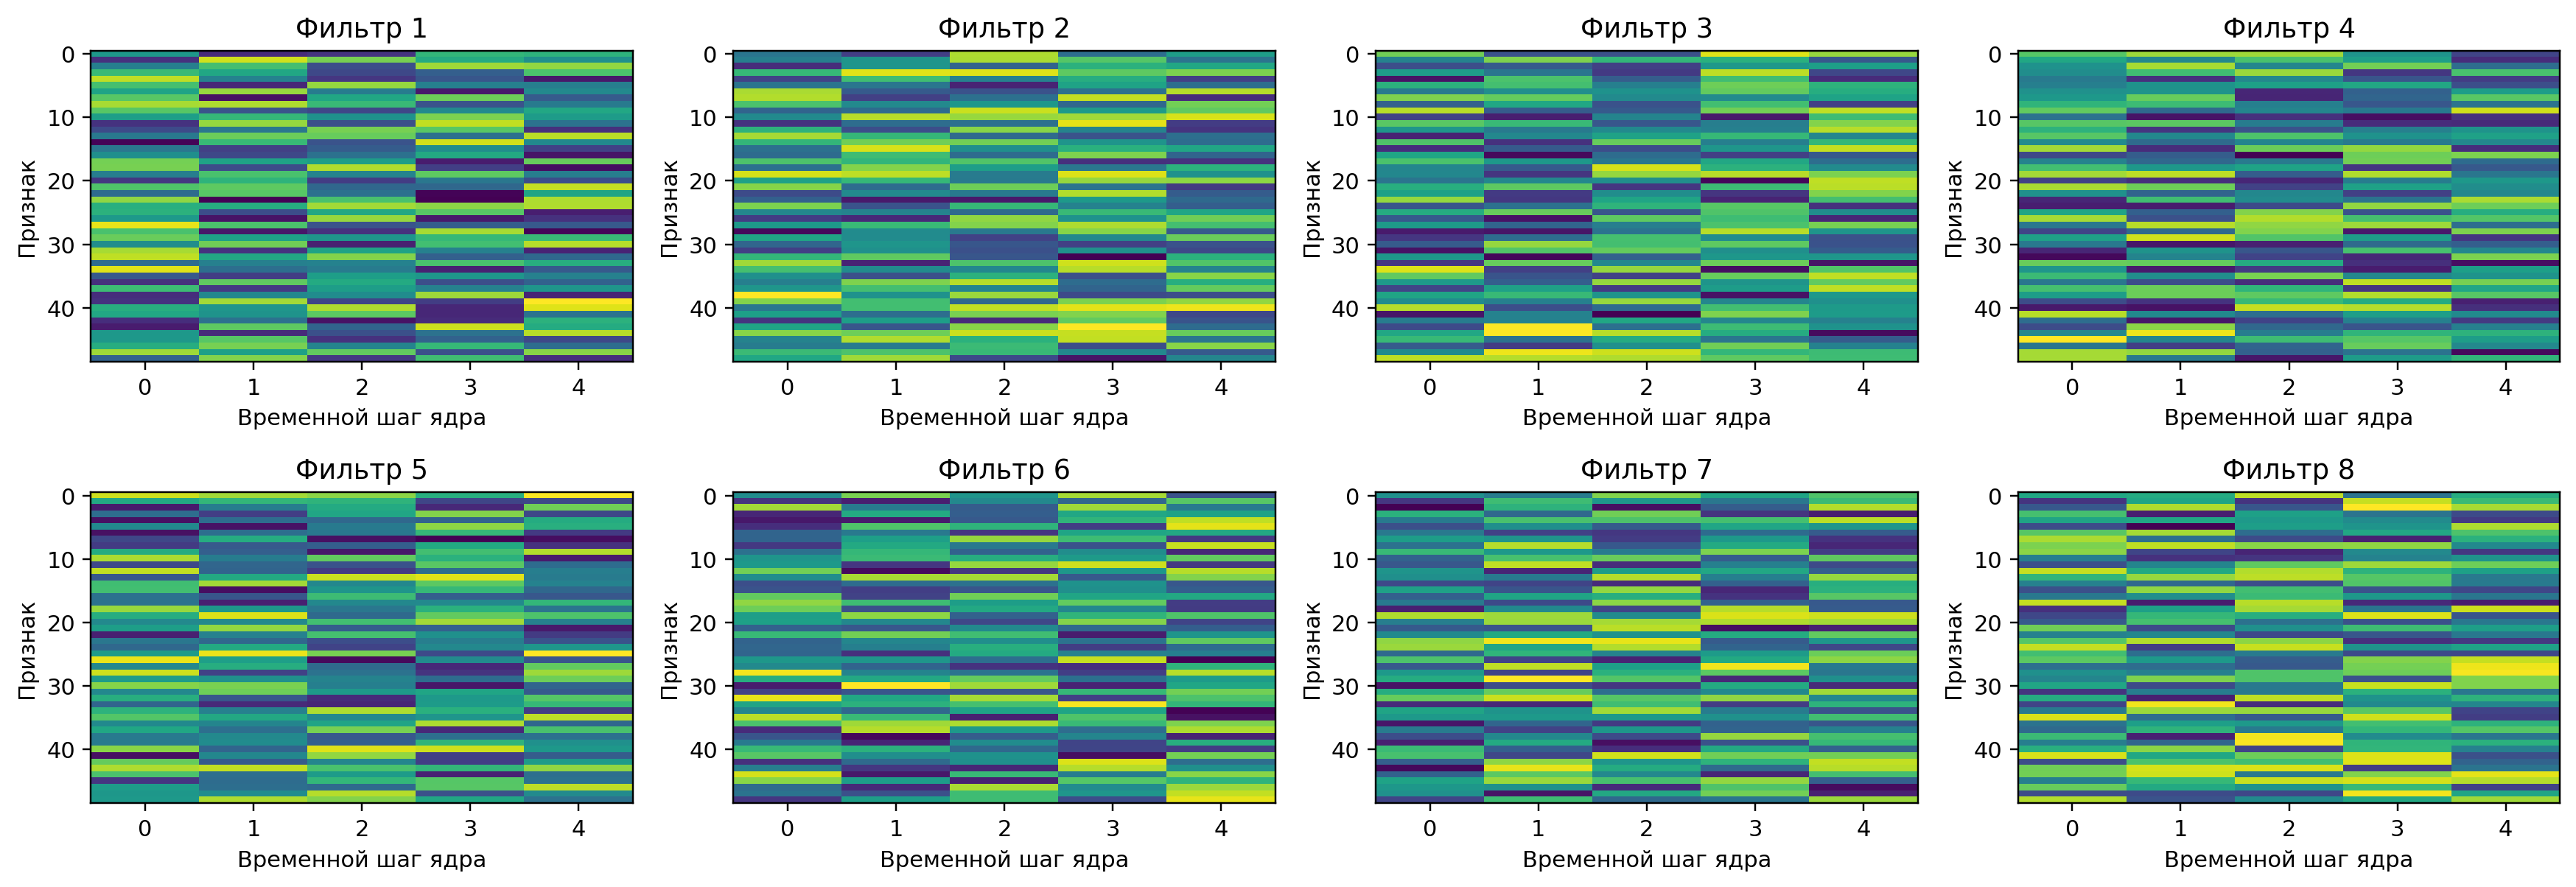
\includegraphics[width=0.9\textwidth]{stage5_improved_conv_filters.png}
\caption{Визуализация весов первого Conv1D-слоя гибридной модели}
\end{figure}

\begin{figure}[H]
\centering
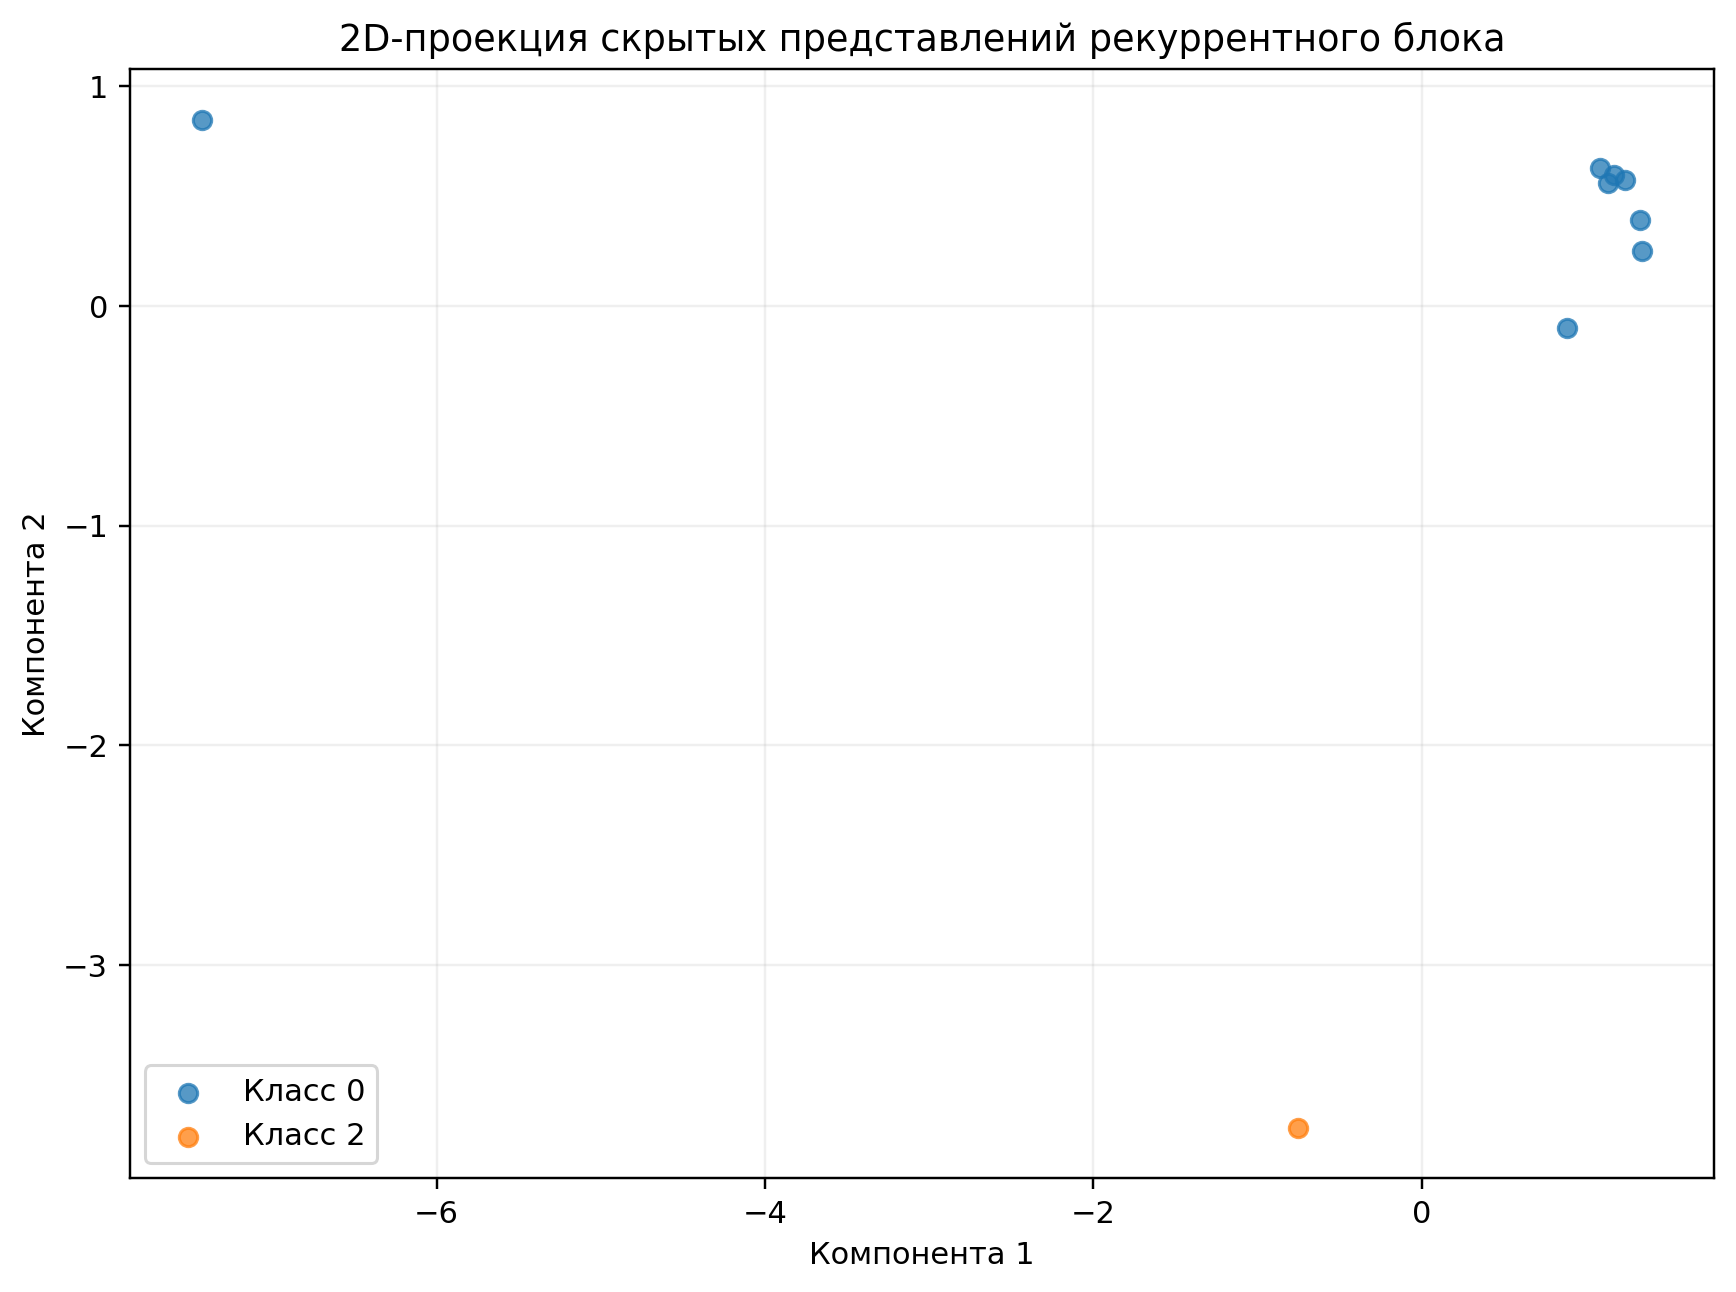
\includegraphics[width=0.76\textwidth]{stage5_improved_hidden_repr.png}
\caption{Двумерная проекция скрытых представлений рекуррентного блока}
\end{figure}

В латентном пространстве окна классов 0 и 2 группируются в существенно более компактные области, чем в исходном признаковом пространстве. Это подтверждает, что нейросетевая часть действительно извлекает более информативное представление, чем baseline-модель на плоском векторе.

\section{Сводный анализ результатов}\label{sec:results}
Сводное сравнение основных конфигураций приведено в таблице~\ref{tab:summary}. Таблица включает улучшенный ROC AUC-анализ для всех доступных этапов, где это допустимо без нарушения протокола работы с test.

\begin{table}[H]
\centering
\caption{Сводные результаты экспериментов на validation и test}
\label{tab:summary}
\begin{tabular}{>{\raggedright\arraybackslash}p{0.32\textwidth}ccc}
\toprule
Конфигурация & macro-F1 & BA & ROC AUC \\
\midrule
Baseline raw (val) & 0.1818 & 0.1875 & 0.5625 \\
Baseline improved (val) & 0.3137 & 0.5000 & 0.1875 \\
Hybrid raw (val) & 0.3111 & 0.4375 & 1.0000 \\
Hybrid improved, GRU (val) & 0.6444 & 0.9375 & 1.0000 \\
Hybrid improved + augmentation (val) & 0.6444 & 0.9375 & 0.9375 \\
Hybrid improved + attention (val) & 0.3137 & 0.5000 & 0.0000 \\
GA best (val, post hoc) & 0.6667 & 1.0000 & 1.0000 \\
AE scratch (val, post hoc) & 0.6444 & 0.9375 & 0.9375 \\
AE fine-tuned (val, post hoc) & 0.6444 & 0.9375 & 0.9375 \\
Final selected pipeline (test) & 0.6667 & 1.0000 & n/a \\
\bottomrule
\end{tabular}
\end{table}

\begin{figure}[H]
\centering

\includegraphics[width=0.88\textwidth]{model_comparison.png}
\caption{Сравнение качества ключевых моделей на validation-части}
\end{figure}

Из таблицы видно, что минимально приемлемый результат достигается лишь после перехода к гибридной архитектуре и улучшенной предобработке. Генетический алгоритм даёт дополнительный, но уже существенно меньший прирост. Аугментация при текущем split не улучшила macro-F1, однако не ухудшила его, что говорит о потенциальной пользе метода на более объёмной или более стабильной валидации. Attention-механизм на текущем наборе данных оказался неэффективен.

\section{Воспроизводимость, Docker и ограничения}\label{sec:repro}
В проекте реализован отдельный контур воспроизводимости. Для каждого запуска фиксируются:
\begin{enumerate}
    \item снимок конфигурации \texttt{config\_snapshot.yaml};
    \item глобальный seed и параметры запуска;
    \item версии библиотек и версия Python;
    \item контрольные суммы входных файлов данных.
\end{enumerate}

Дополнительно подготовлены файлы \texttt{Dockerfile}, \texttt{docker-compose.yml} и \texttt{Makefile}, позволяющие запускать основные этапы внутри контейнера. Такой подход обеспечивает переносимость вычислительной среды и снижает риск расхождения результатов между машинами.

Типовой сценарий запуска в контейнере:
\begin{lstlisting}[language=bash]
make build
make test
make stage4
make stage5
make diagnostics
\end{lstlisting}

Несмотря на детерминизацию вычислительного контура, в системе сохраняются два принципиальных ограничения.

Во-первых, официальный \texttt{validation}-срез содержит только классы 0 и 2, а класс 1 в нём отсутствует. Поэтому ROC AUC и часть quality-выводов относятся только к фактически присутствующим классам. Во-вторых, на этапе 8 действует правило «не трогать test повторно». По этой причине итоговая тестовая оценка не пересчитывалась после внедрения расширенного ROC AUC-анализа, чтобы не нарушать методический контракт.

\section{Финальная оценка и анализ устойчивости}\label{sec:final}
Финальный выбор пайплайна был сделан по \texttt{validation}: лучшим кандидатом оказался контур \texttt{stage6\_ga\_no\_ae}. Перед фиксацией результата выполнялась проверка устойчивости на трёх разных значениях seed.

\begin{figure}[H]
\centering

\includegraphics[width=0.78\textwidth]{seed_stability.png}
\caption{Сравнение качества лучшей конфигурации при разных значениях seed}
\end{figure}

Здесь выявлено важное практическое ограничение: при \texttt{seed=2} качество заметно падает ниже baseline-уровня, тогда как при \texttt{seed=0} и \texttt{seed=1} модель работает существенно лучше. Следовательно, найденная конфигурация не является полностью устойчивой и требует дополнительной стабилизации при дальнейшем развитии системы.

Итоговая оценка на \texttt{test} была выполнена ровно один раз и дала $macro\text{-}F1=0.6667$, $BA=1.0000$. При этом в тестовой части отсутствует класс 2, поэтому значение ROC AUC сохранено как \texttt{n/a}. Повторный пересчёт намеренно не выполнялся.

\begin{figure}[H]
\centering

\includegraphics[width=0.62\textwidth]{test_confusion_matrix.png}
\caption{Матрица ошибок финальной выбранной модели на test-выборке}
\end{figure}

\section{Заключение}
В рамках курсовой работы была разработана воспроизводимая система анализа телеметрии малого космического аппарата, включающая полный цикл от загрузки и валидации данных до финального выбора модели и документирования результатов. Практически значимым итогом является построение рабочего контура классификации состояний аппарата с качеством, заметно превосходящим базовую линейную модель.

Наиболее важные технические результаты работы состоят в следующем. Во-первых, подтверждено, что простая линейная baseline-модель не обеспечивает достаточной устойчивости и чувствительна к качеству предобработки. Во-вторых, показано, что комбинация winsorization, робастного масштабирования и гибридной архитектуры \texttt{1D-CNN \textrightarrow GRU \textrightarrow Dense} даёт существенный прирост качества и является правильной базовой инженерной стратегией для данного класса задач. В-третьих, введённый в проект ROC AUC-анализ позволил перейти от формального упоминания метрики к содержательному разбору ранжирующей способности моделей, причём корректно даже в ситуации, когда часть классов отсутствует во временном split.

Дополнительные исследования показали, что двунаправленные рекуррентные блоки способны дать ещё небольшой прирост на validation, однако этот выигрыш достигается ростом числа параметров и потенциальным усложнением эксплуатации. Аугментация временных окон в текущем эксперименте не улучшила macro-F1, но и не ухудшила его, а значит может быть полезна как средство стабилизации при большем объёме данных. Механизм внимания, напротив, на рассматриваемом наборе продемонстрировал ухудшение качества, что подчёркивает важный инженерный вывод: более сложная архитектура не гарантирует лучшего результата без достаточного объёма и разнообразия обучающих примеров. Предобучение автоэнкодера также не принесло выигрыша на текущем наборе, что дало ценный отрицательный результат и показало границы применимости semi-supervised подхода в данной постановке.

С точки зрения профессиональных навыков выполнение работы позволило закрепить умения проектировать полный ML-конвейер, формализовывать контракт данных, строить корректную временную валидацию без утечки, работать с дисбалансом классов, интерпретировать нейросетевые модели, подбирать гиперпараметры через эволюционные методы, документировать результаты по требованиям учебной методички и обеспечивать воспроизводимость вычислений. Отдельно был отработан навык интеграции программной части и отчётной документации: результаты экспериментов автоматически переводятся в артефакты, удобные для анализа, проверки и защиты.

Перспективы дальнейшего развития системы состоят в расширении протокола валидации (например, за счёт нескольких временных фолдов как дополнительного диагностического контура), наращивании объёма размеченной выборки для редких классов, стабилизации лучших конфигураций по seed и развитии методов интерпретации скрытых представлений. В эксплуатационном контуре особенно важно уменьшить чувствительность модели к редким временным сценариям и обеспечить устойчивое качество не только по двум наиболее представленным классам, но и по редким аварийным состояниям.

\clearpage
\begin{thebibliography}{99}
\addcontentsline{toc}{section}{Список литературы}
\bibitem{goodfellow} Гудфеллоу И., Бенджио И., Курвилль А. Глубокое обучение. М.: ДМК Пресс, 2018. 652 с.
\bibitem{chollet} Шолле Ф. Глубокое обучение на Python. 2-е изд. СПб.: Питер, 2022. 560 с.
\bibitem{bishop} Бишоп К. Распознавание образов и машинное обучение. М.: Вильямс, 2016. 738 с.
\bibitem{hastie} Хасти Т., Тибширани Р., Фридман Дж. Элементы статистического обучения. М.: ДМК Пресс, 2021. 768 с.
\bibitem{sklearn} Pedregosa F. et al. Scikit-learn: Machine Learning in Python // Journal of Machine Learning Research. 2011. Vol. 12. P. 2825--2830.
\bibitem{tensorflow} Abadi M. et al. TensorFlow: Large-Scale Machine Learning on Heterogeneous Systems [Электронный ресурс]. URL: \url{https://www.tensorflow.org/} (дата обращения: 01.03.2026).
\bibitem{keras} Chollet F. Keras [Электронный ресурс]. URL: \url{https://keras.io/} (дата обращения: 01.03.2026).
\bibitem{roc} Fawcett T. An Introduction to ROC Analysis // Pattern Recognition Letters. 2006. Vol. 27, No. 8. P. 861--874.
\bibitem{gru} Cho K. et al. Learning Phrase Representations using RNN Encoder--Decoder for Statistical Machine Translation // EMNLP 2014. P. 1724--1734.
\bibitem{attention} Bahdanau D., Cho K., Bengio Y. Neural Machine Translation by Jointly Learning to Align and Translate // ICLR 2015.
\end{thebibliography}

\appendix
\clearpage
\section*{Приложения}
\addcontentsline{toc}{section}{Приложения}
В приложениях приведены ключевые листинги реализованной кодовой базы. Детали, связанные с базовой моделью, см. в приложении A; гибридная модель приведена в приложении Б; реализация генетического алгоритма --- в приложении В; автоэнкодер --- в приложении Г. Таким образом, основной текст отчёта сохраняет описательный характер, а программная реализация остаётся доступной для технической проверки.

\IfFileExists{generated_code_appendices.tex}{\section*{Приложение А. Базовая модель классификации}
\addcontentsline{toc}{section}{Приложение А. Базовая модель классификации}
\noindent\textbf{Файл:} \path{src/models/baseline.py}
\par\vspace{0.4cm}
\begin{figure}[H]
\centering
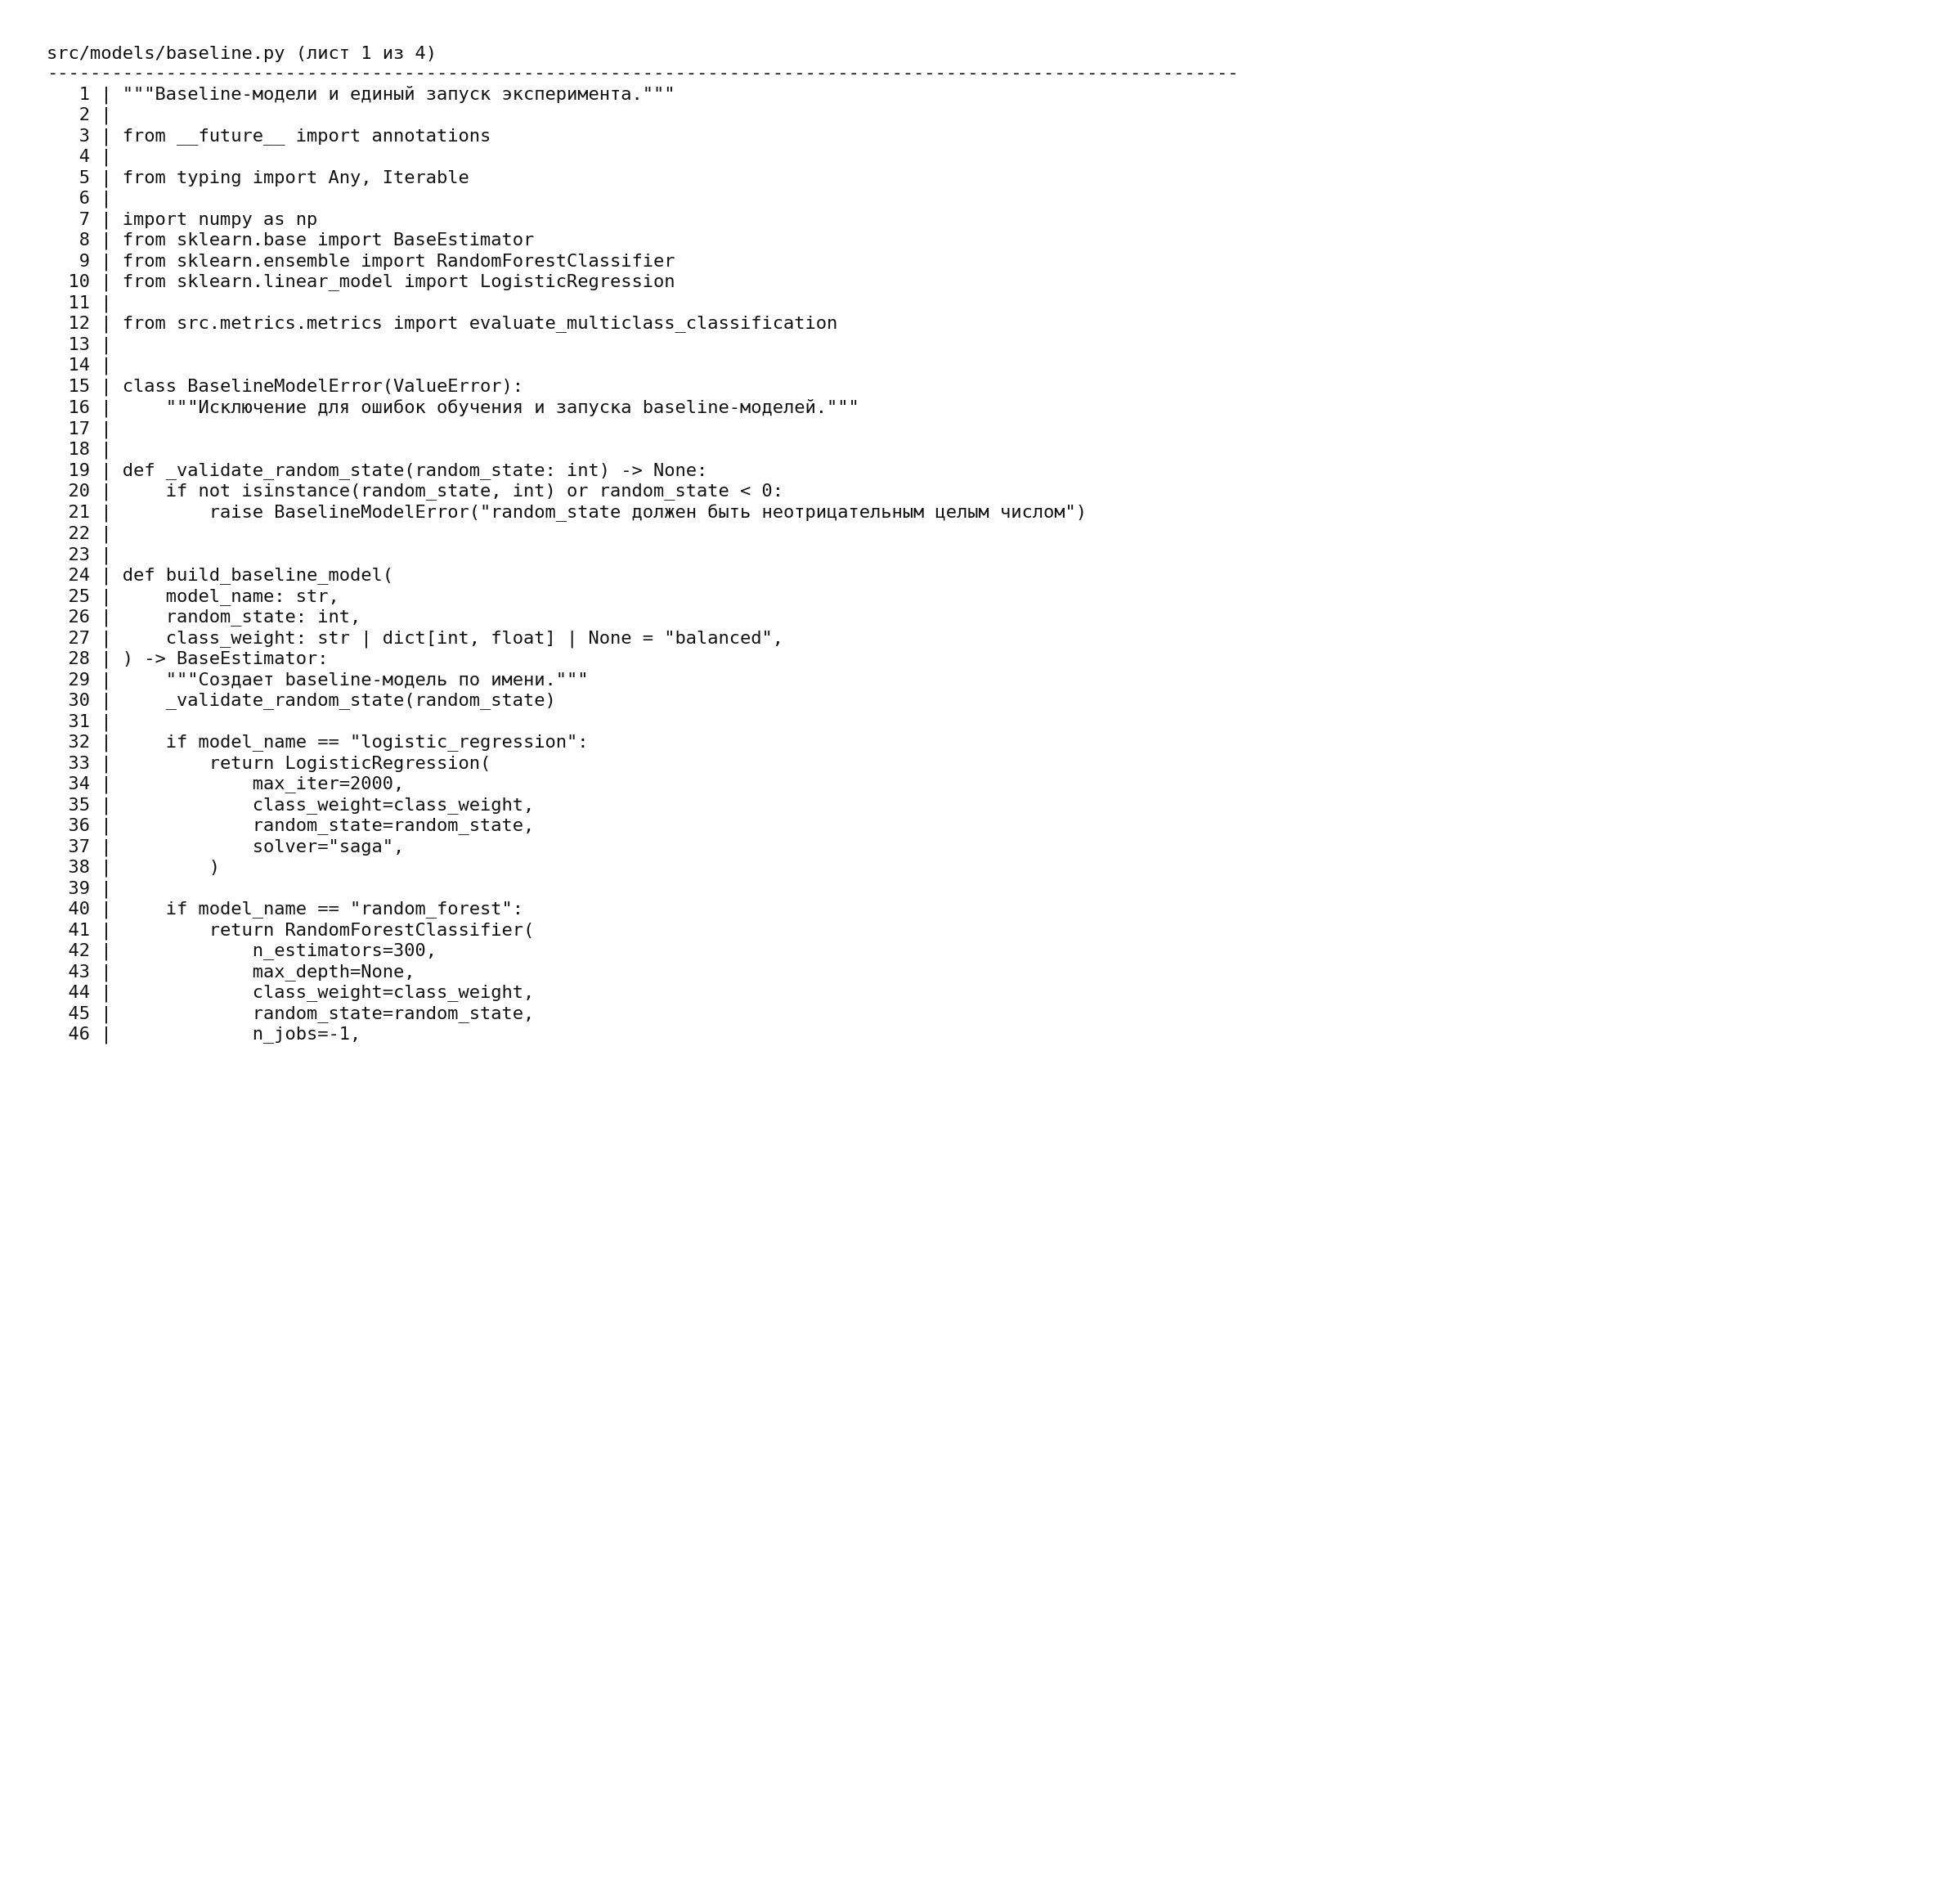
\includegraphics[width=\textwidth]{figures/appendix_baseline_p01.png}
\caption{Листинг файла src/models/baseline.py, лист 1}
\end{figure}
\begin{figure}[H]
\centering
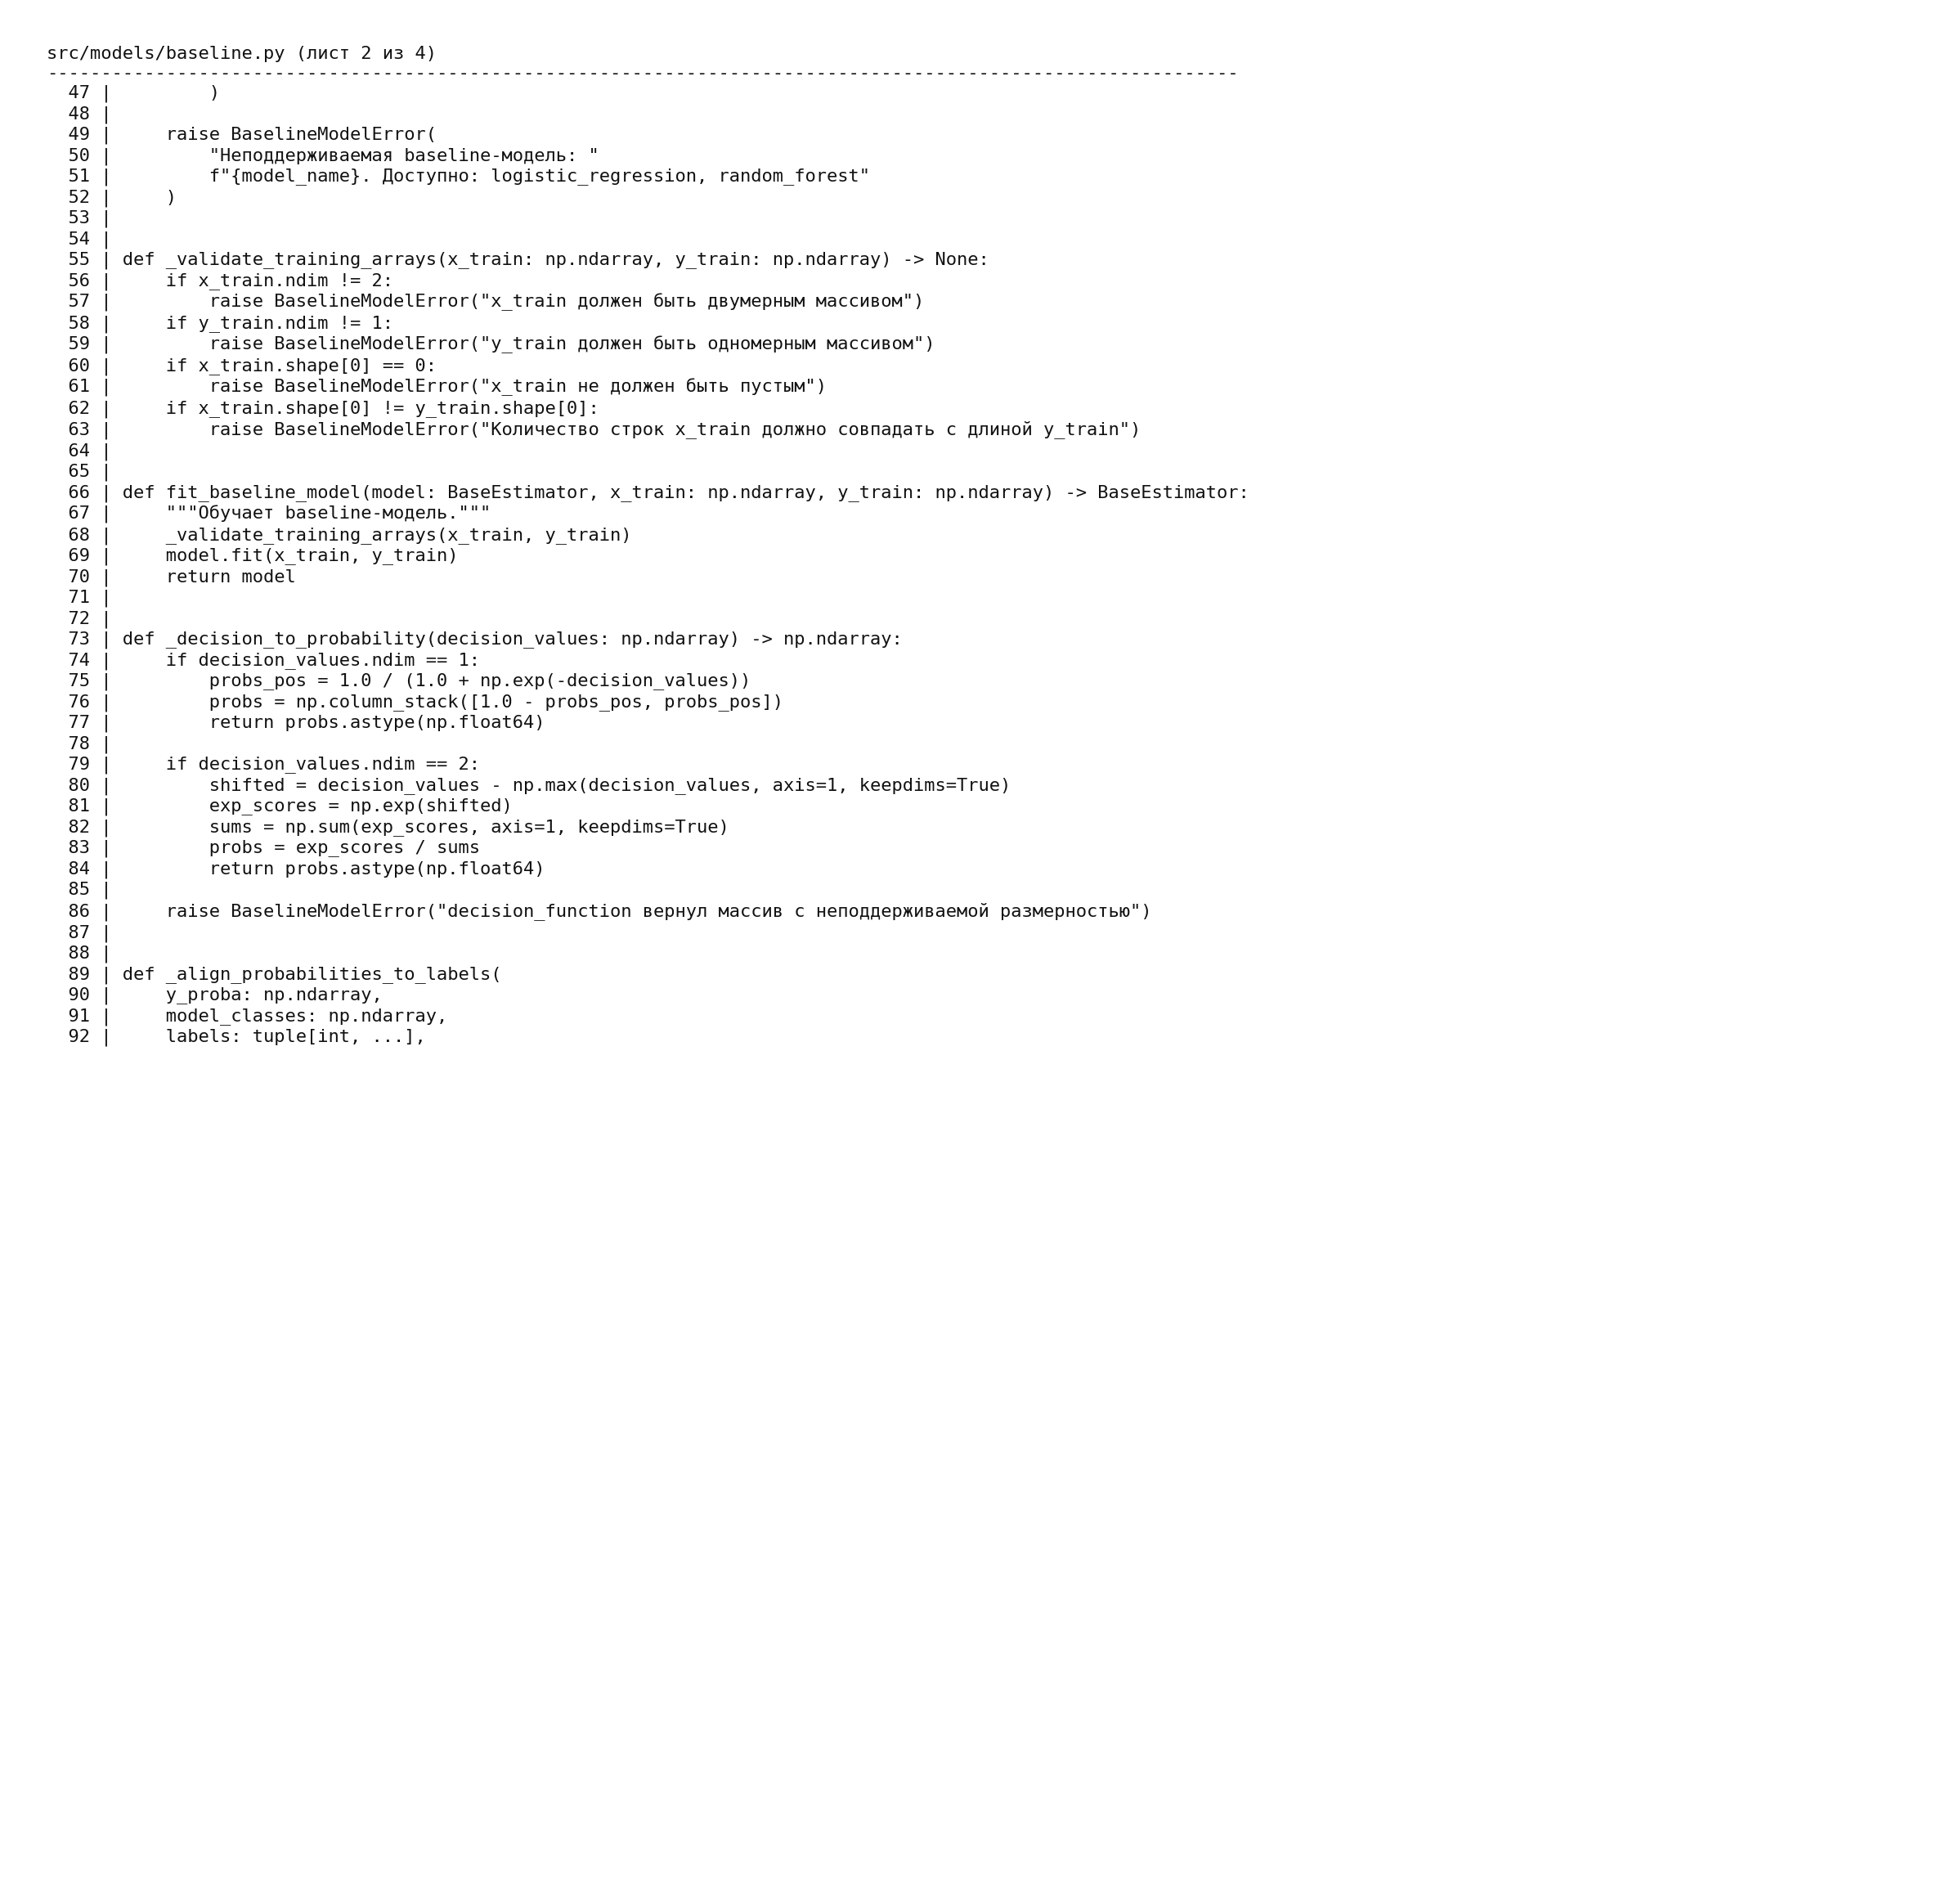
\includegraphics[width=\textwidth]{figures/appendix_baseline_p02.png}
\caption{Листинг файла src/models/baseline.py, лист 2}
\end{figure}
\begin{figure}[H]
\centering
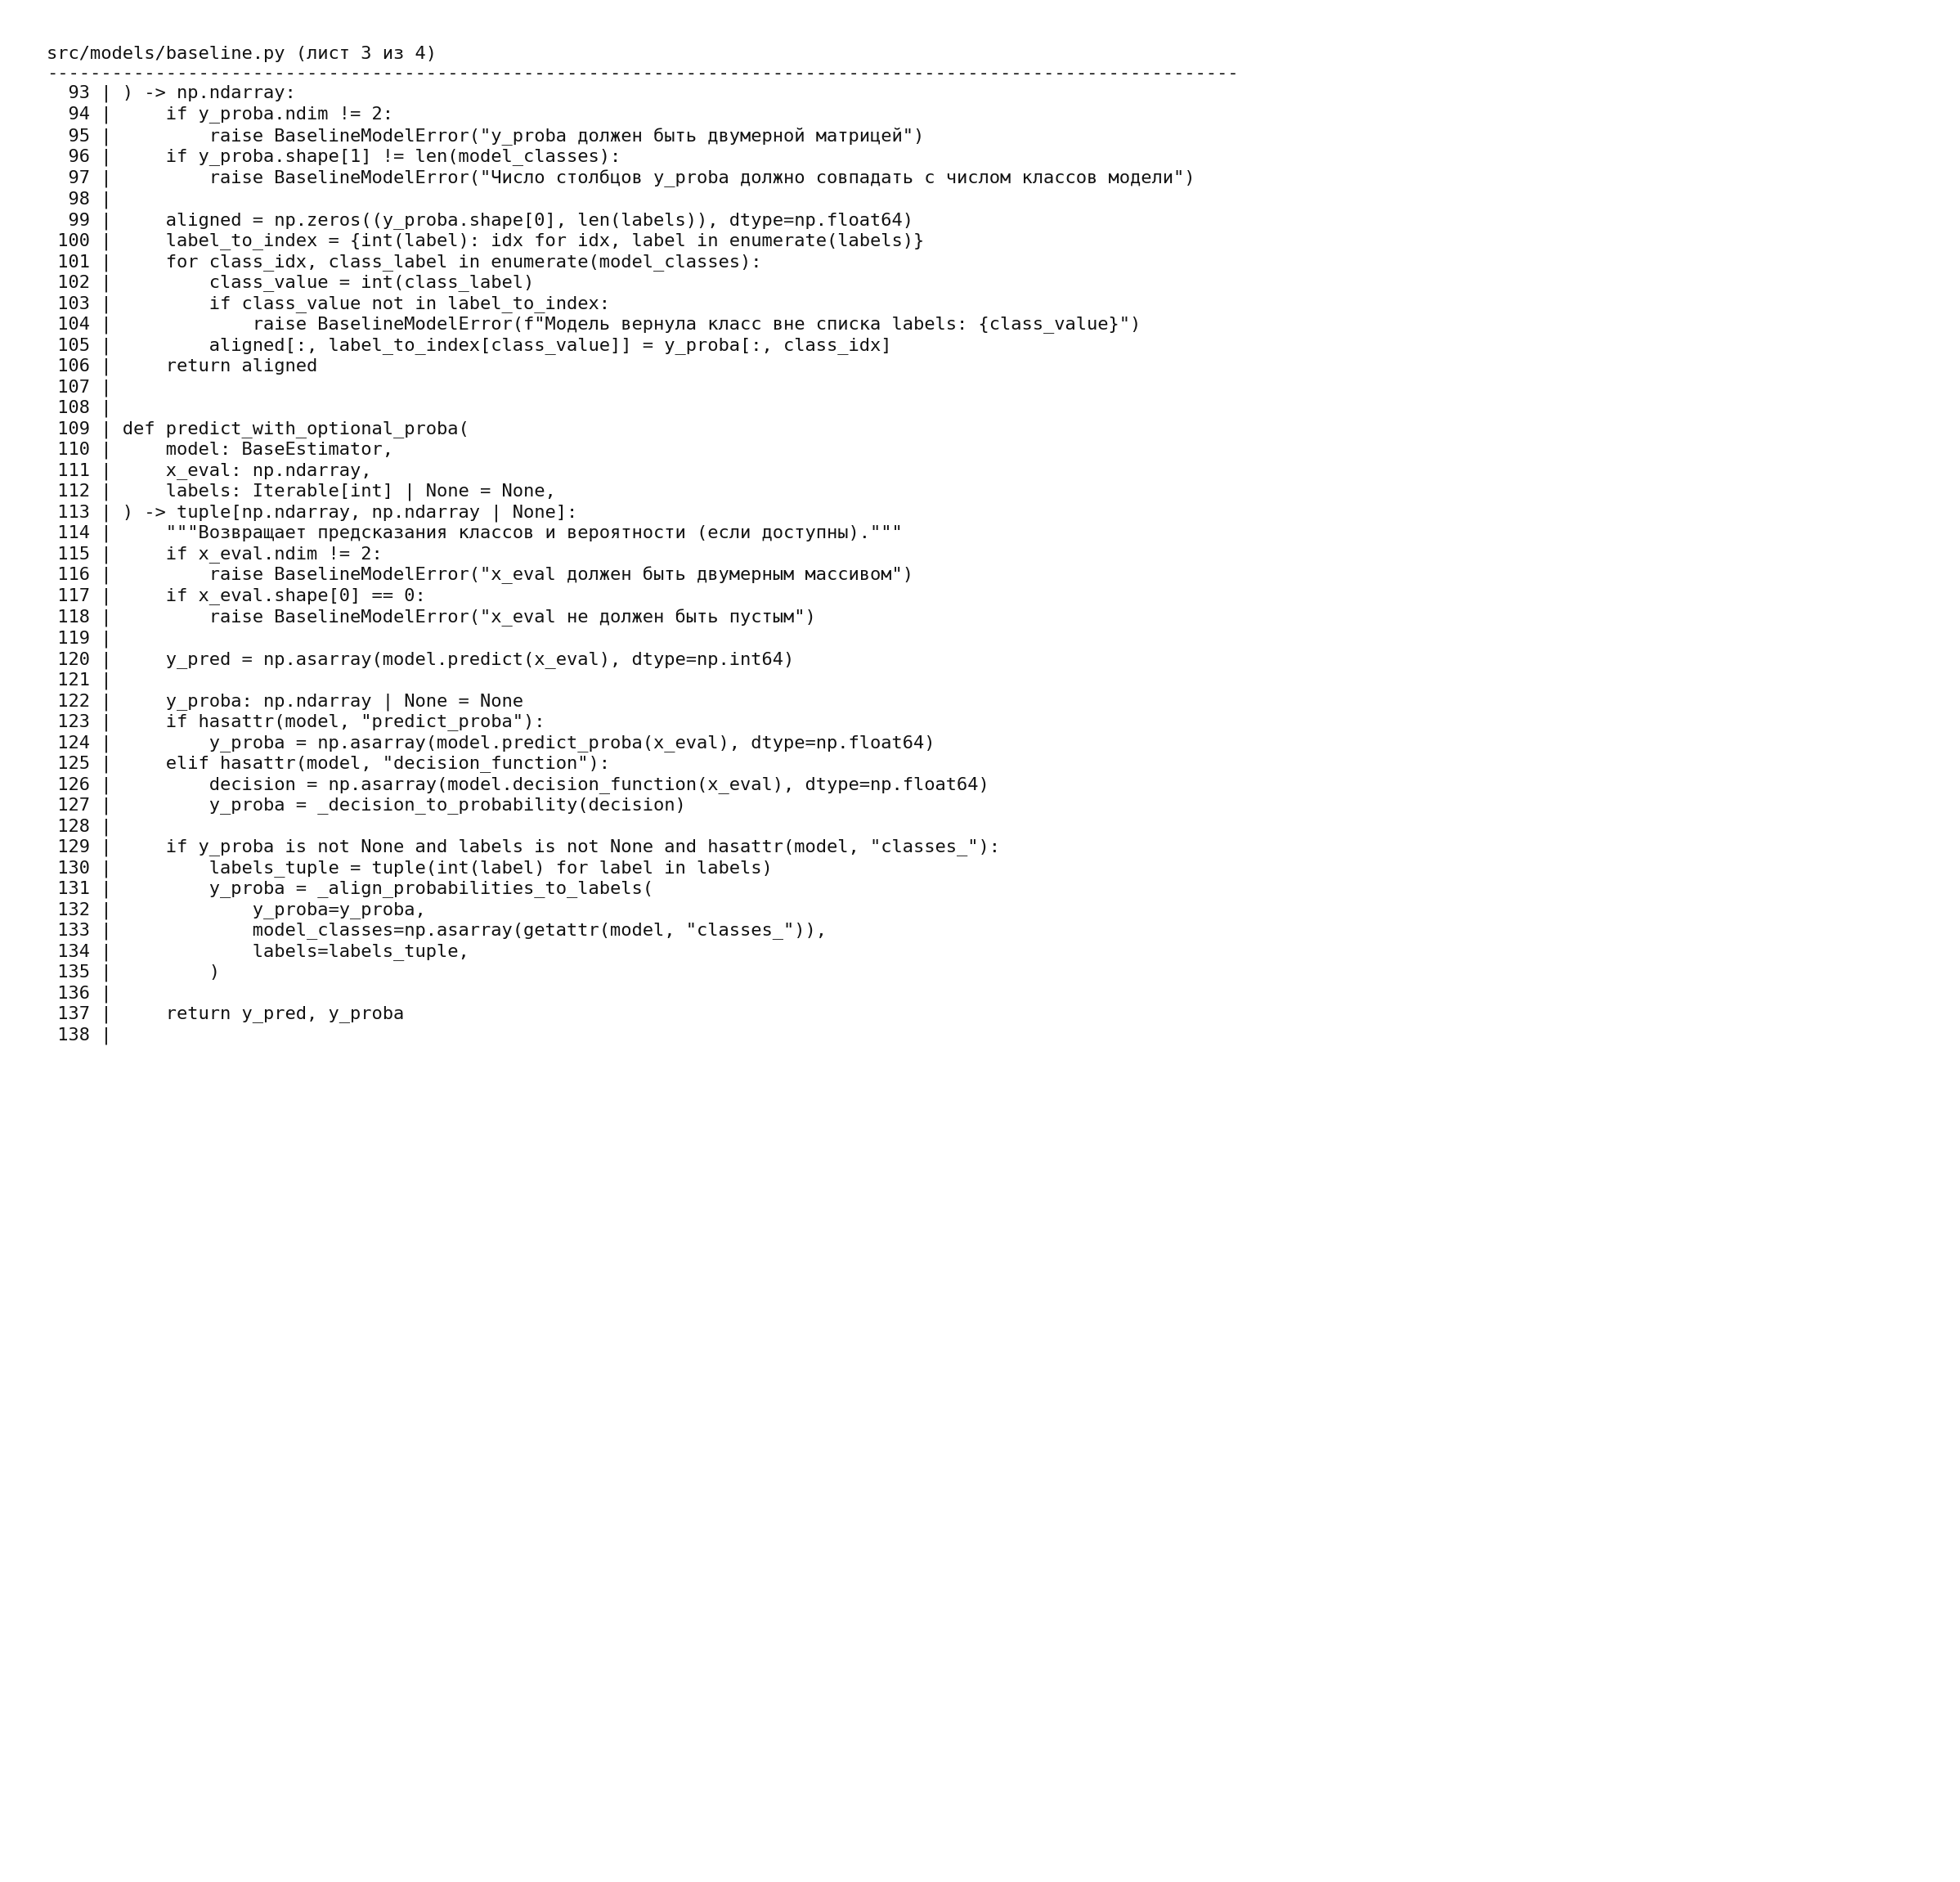
\includegraphics[width=\textwidth]{figures/appendix_baseline_p03.png}
\caption{Листинг файла src/models/baseline.py, лист 3}
\end{figure}
\begin{figure}[H]
\centering
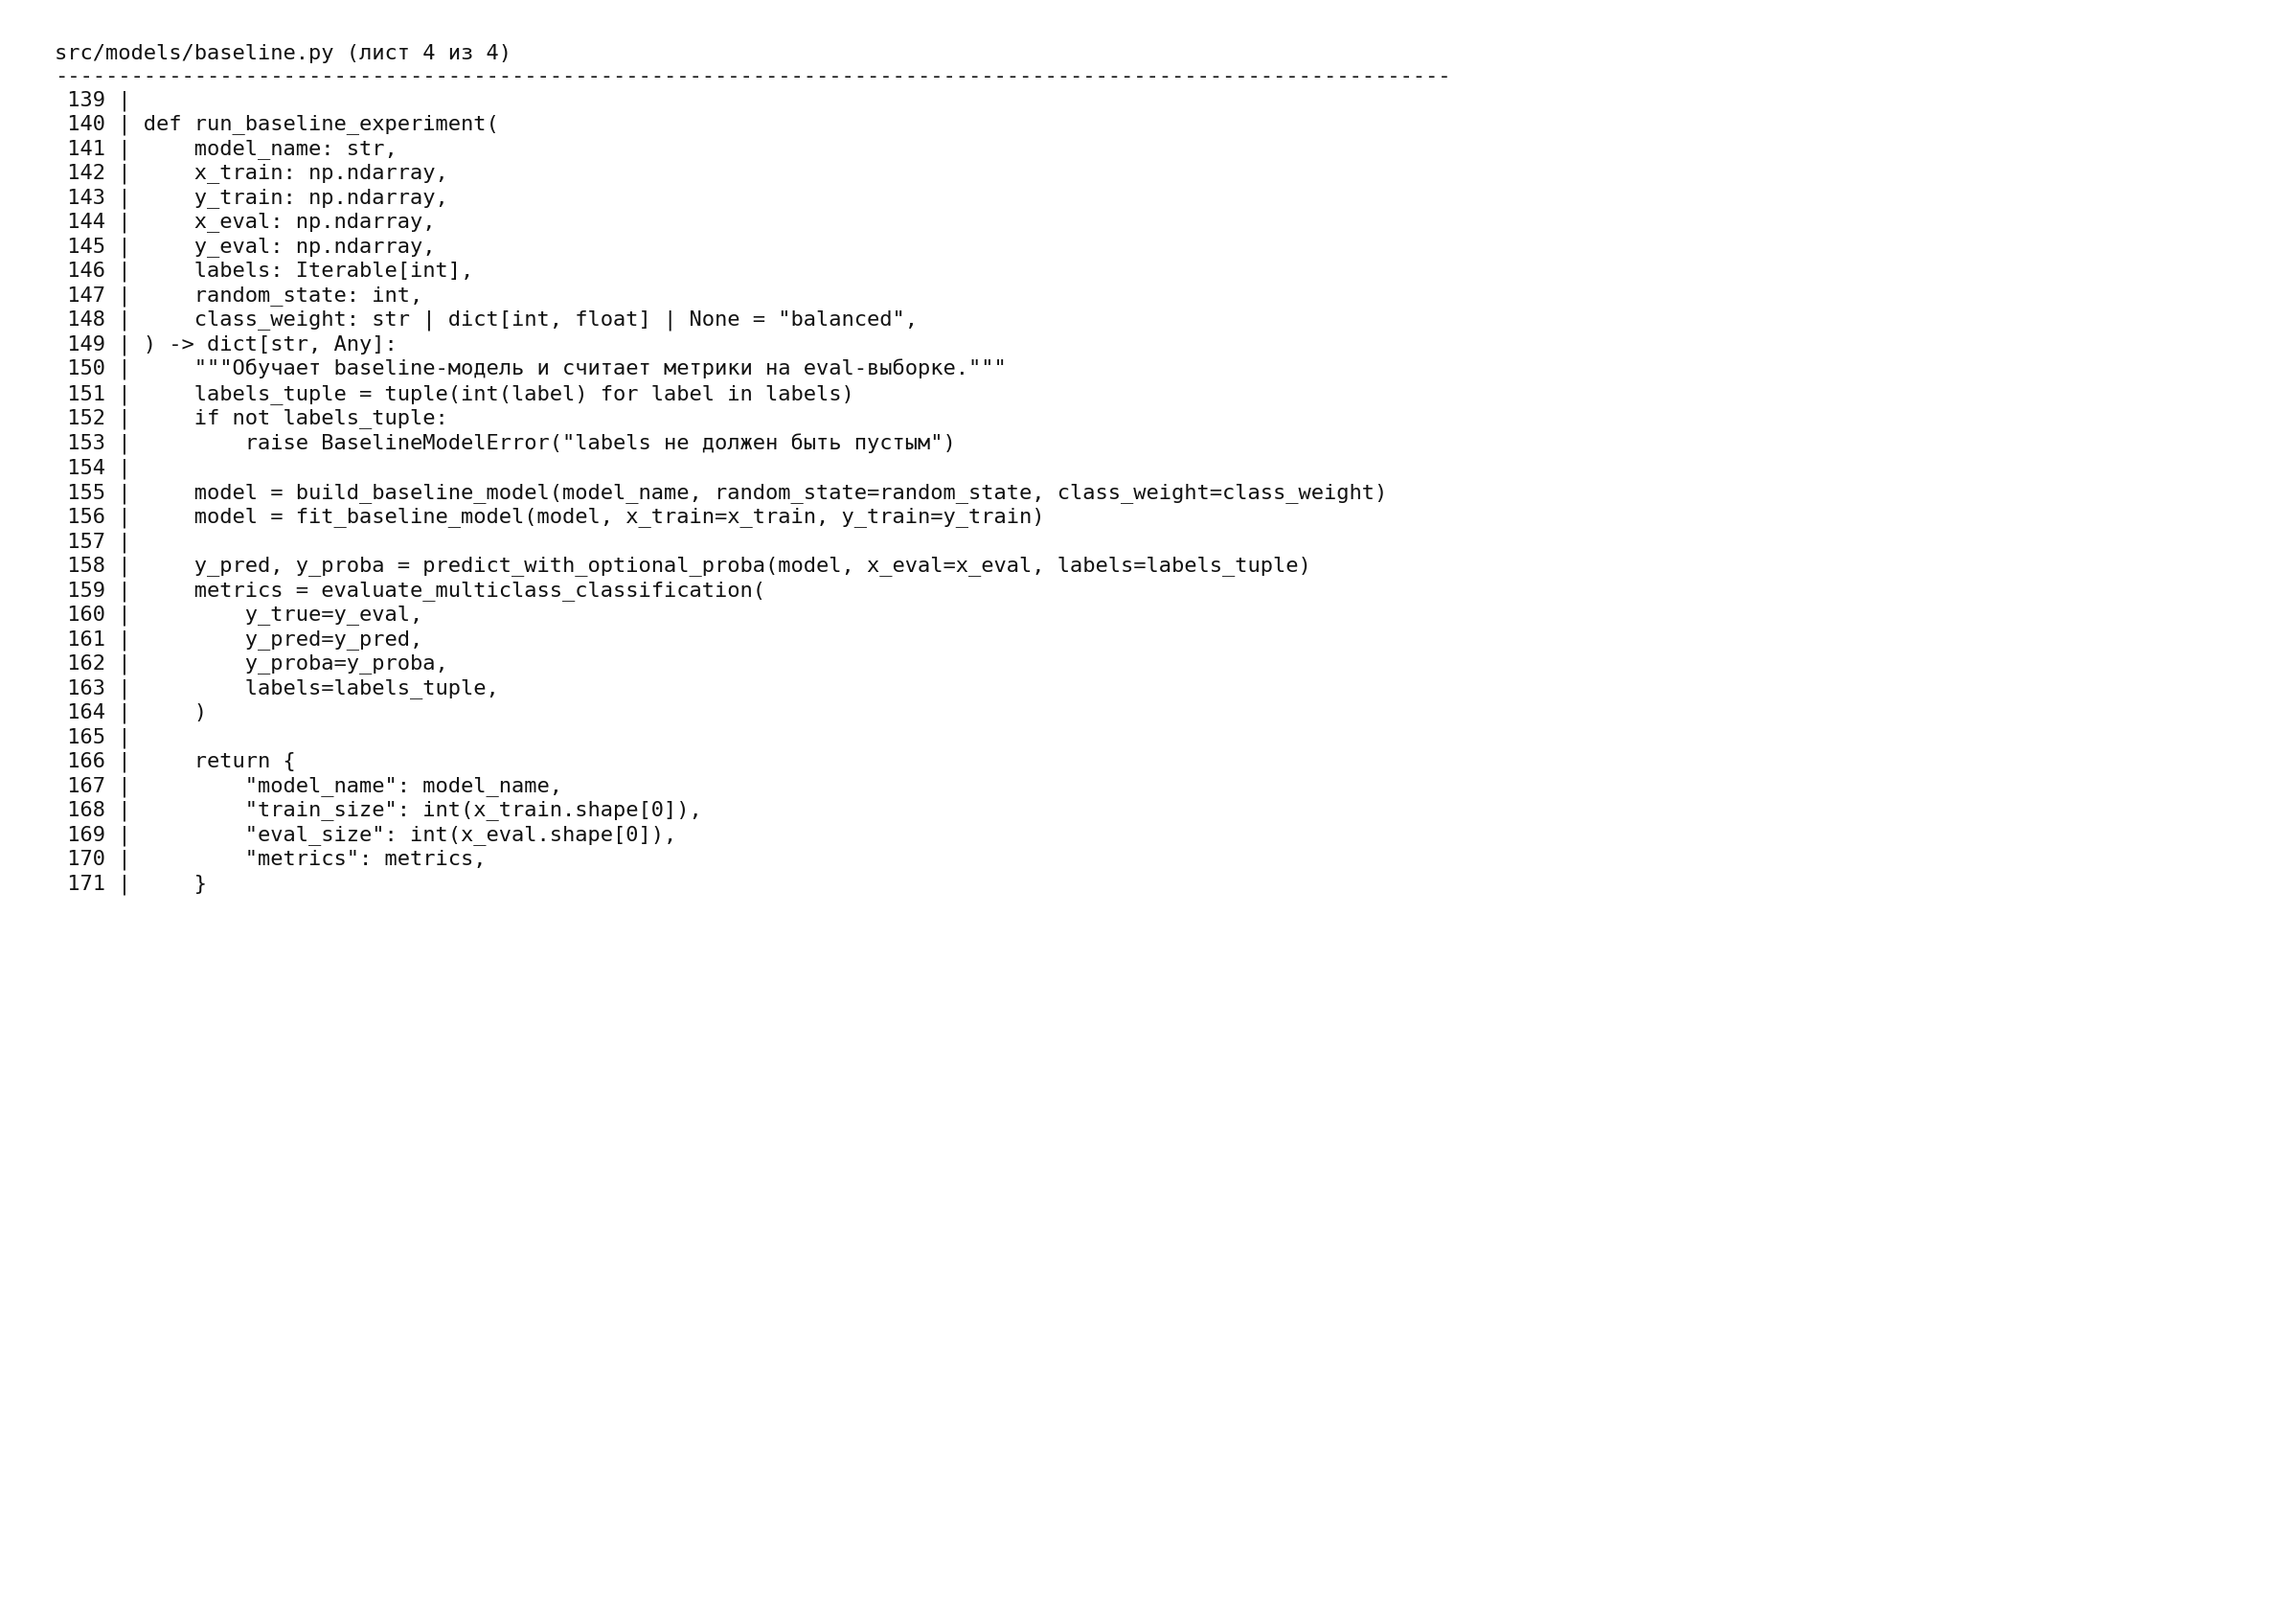
\includegraphics[width=\textwidth]{figures/appendix_baseline_p04.png}
\caption{Листинг файла src/models/baseline.py, лист 4}
\end{figure}
\clearpage
\section*{Приложение Б. Гибридная модель 1D-CNN -> GRU -> Dense}
\addcontentsline{toc}{section}{Приложение Б. Гибридная модель 1D-CNN -> GRU -> Dense}
\noindent\textbf{Файл:} \path{src/models/hybrid.py}
\par\vspace{0.4cm}
\begin{figure}[H]
\centering
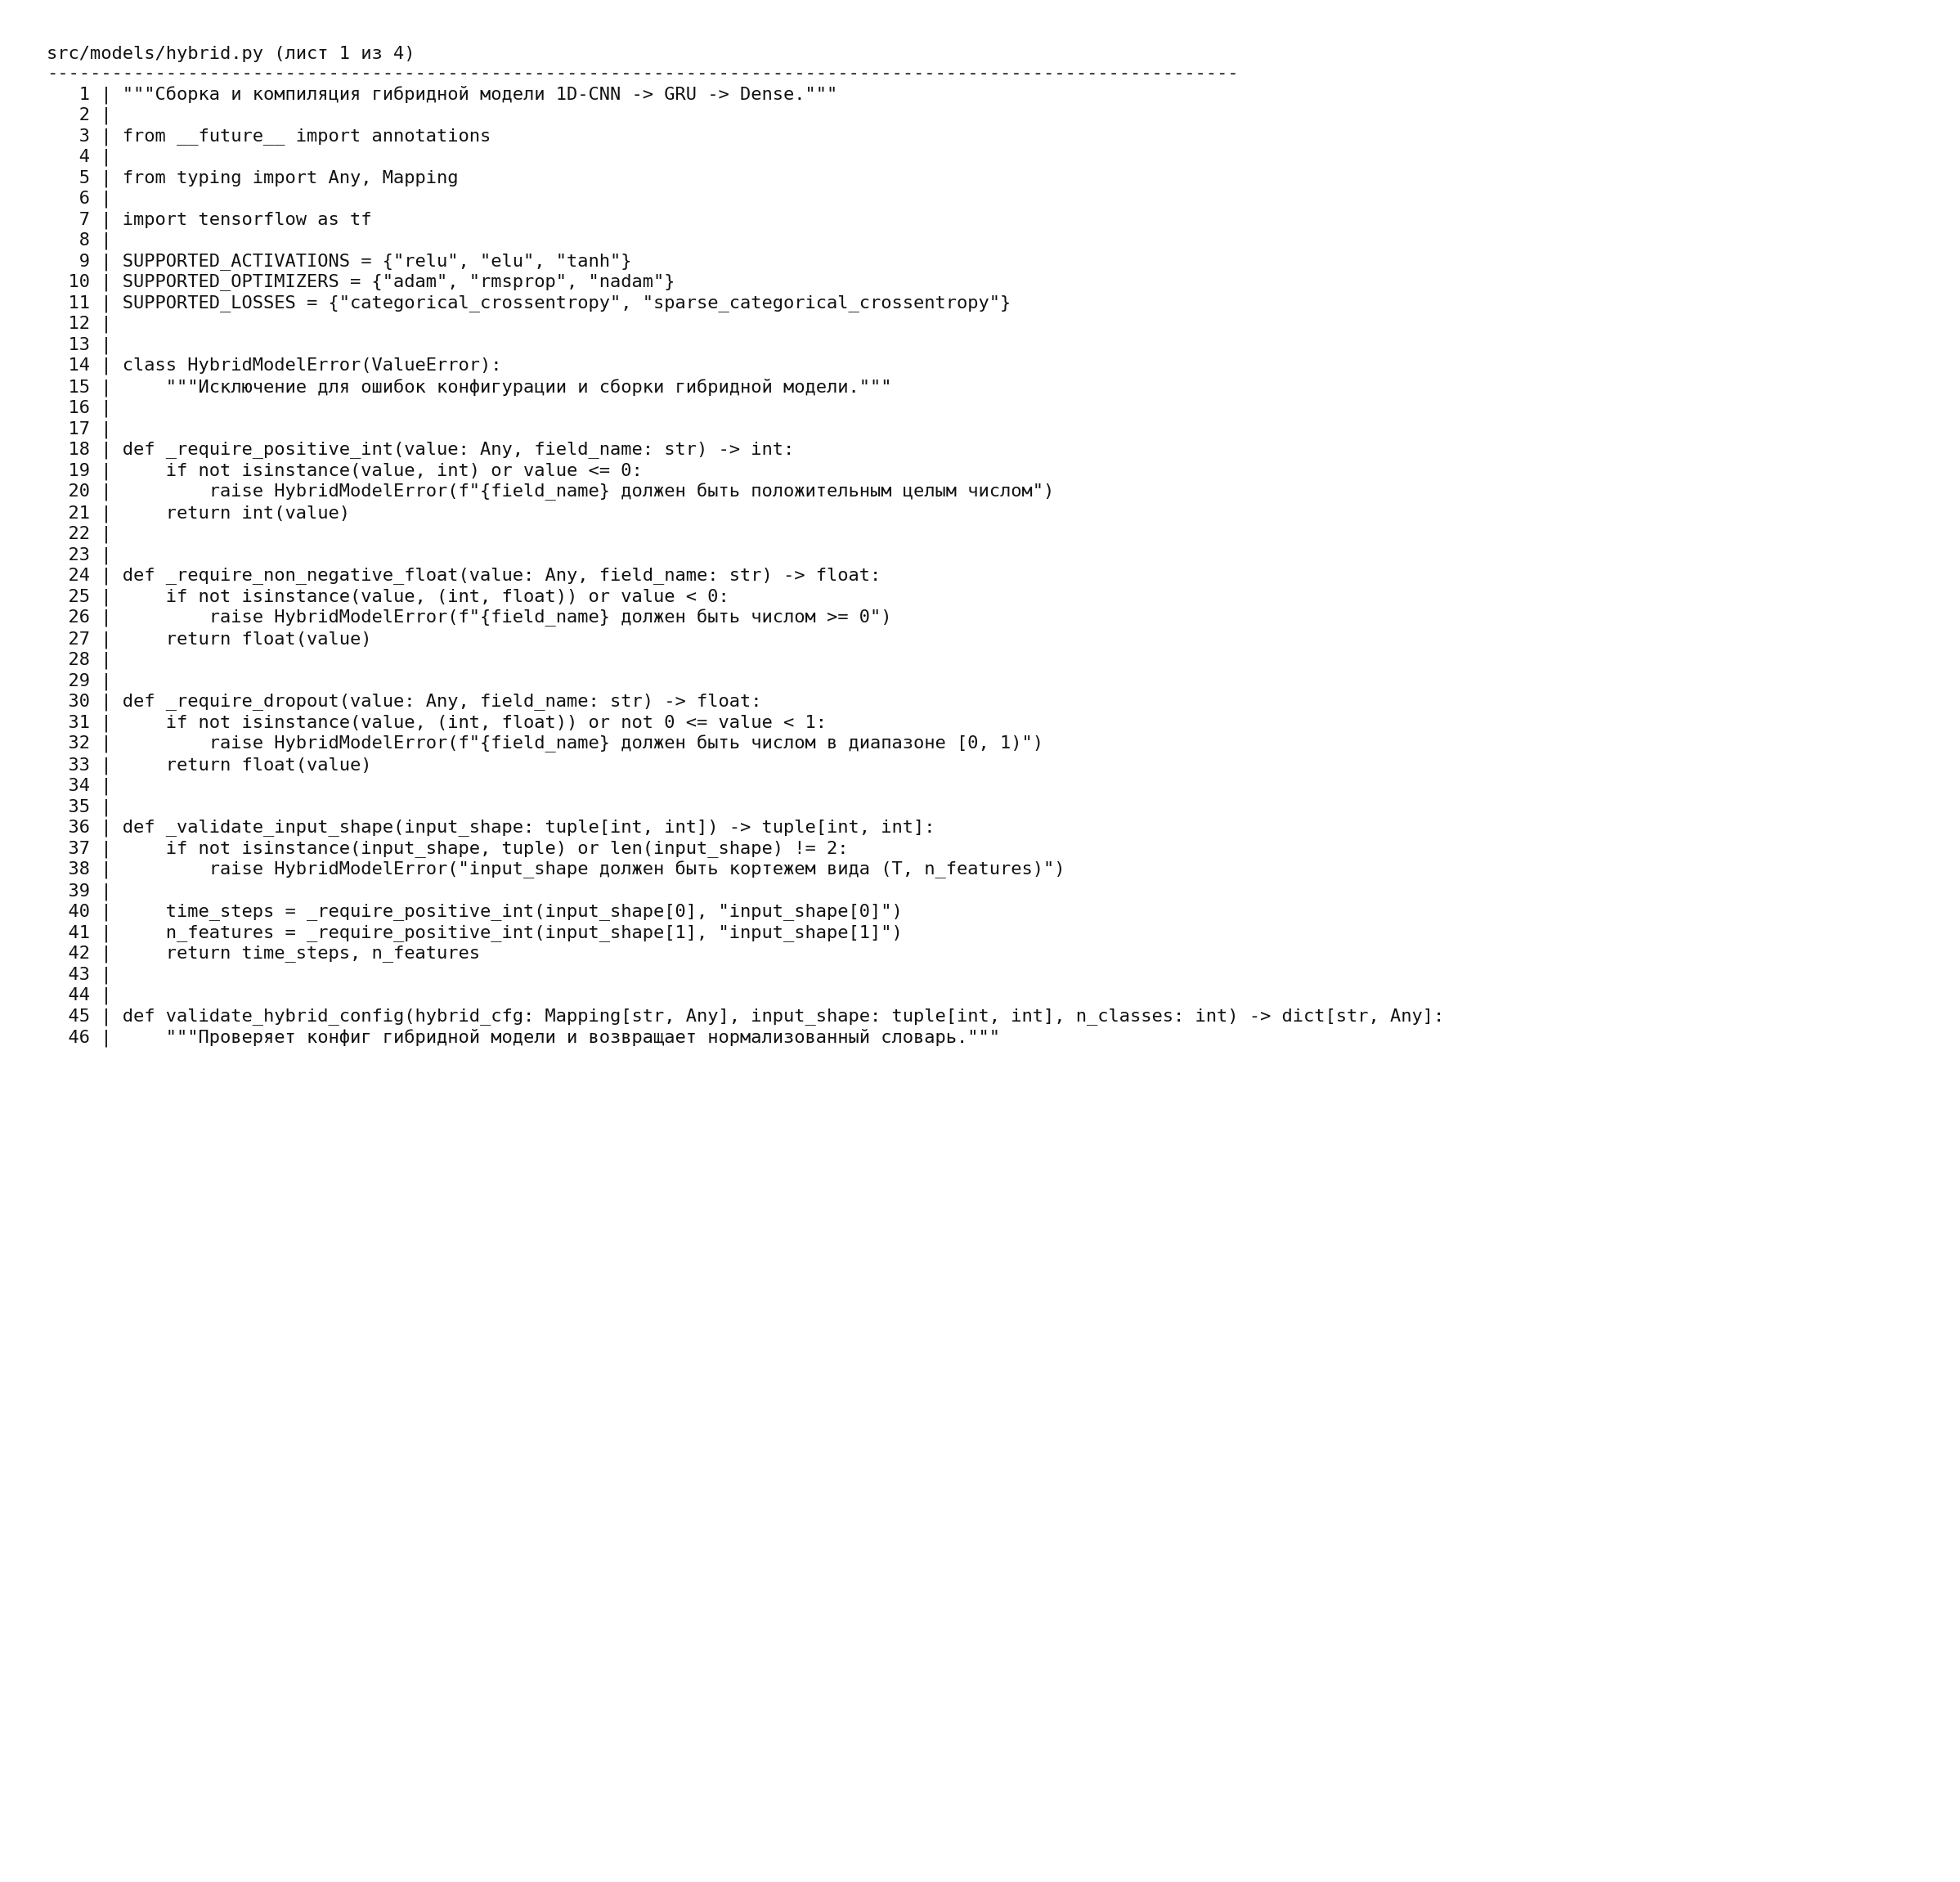
\includegraphics[width=\textwidth]{figures/appendix_hybrid_p01.png}
\caption{Листинг файла src/models/hybrid.py, лист 1}
\end{figure}
\begin{figure}[H]
\centering
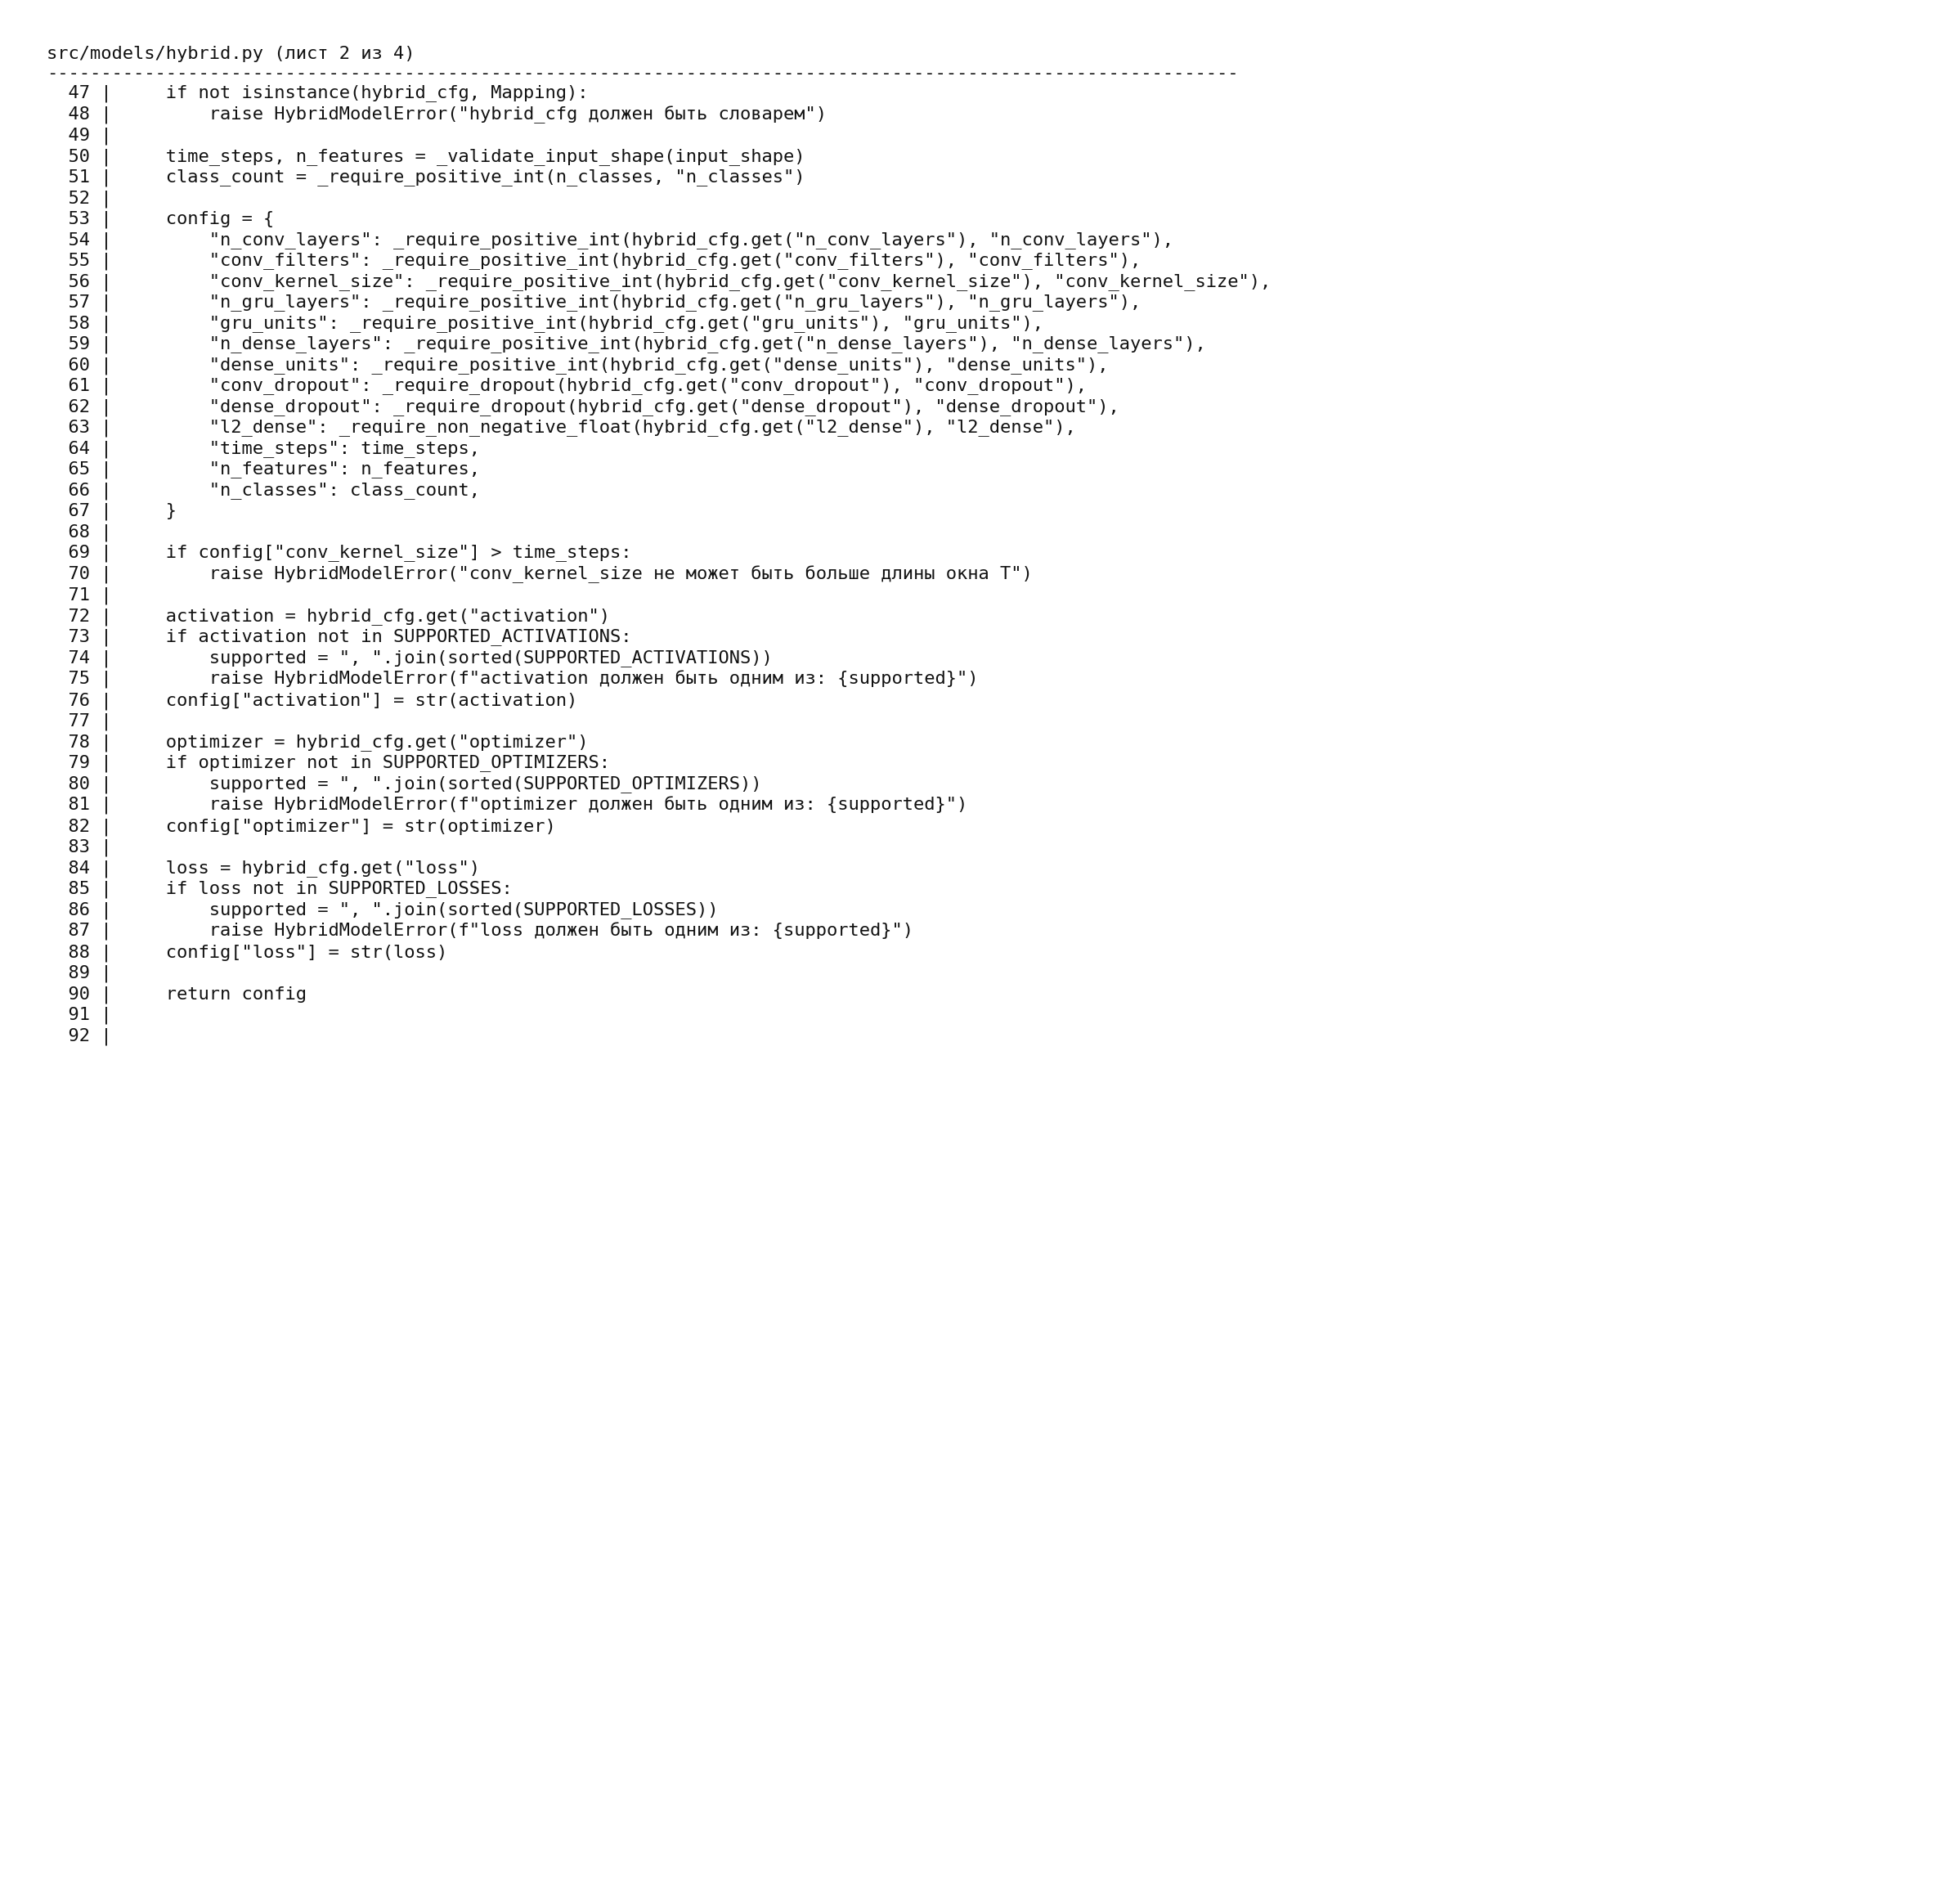
\includegraphics[width=\textwidth]{figures/appendix_hybrid_p02.png}
\caption{Листинг файла src/models/hybrid.py, лист 2}
\end{figure}
\begin{figure}[H]
\centering
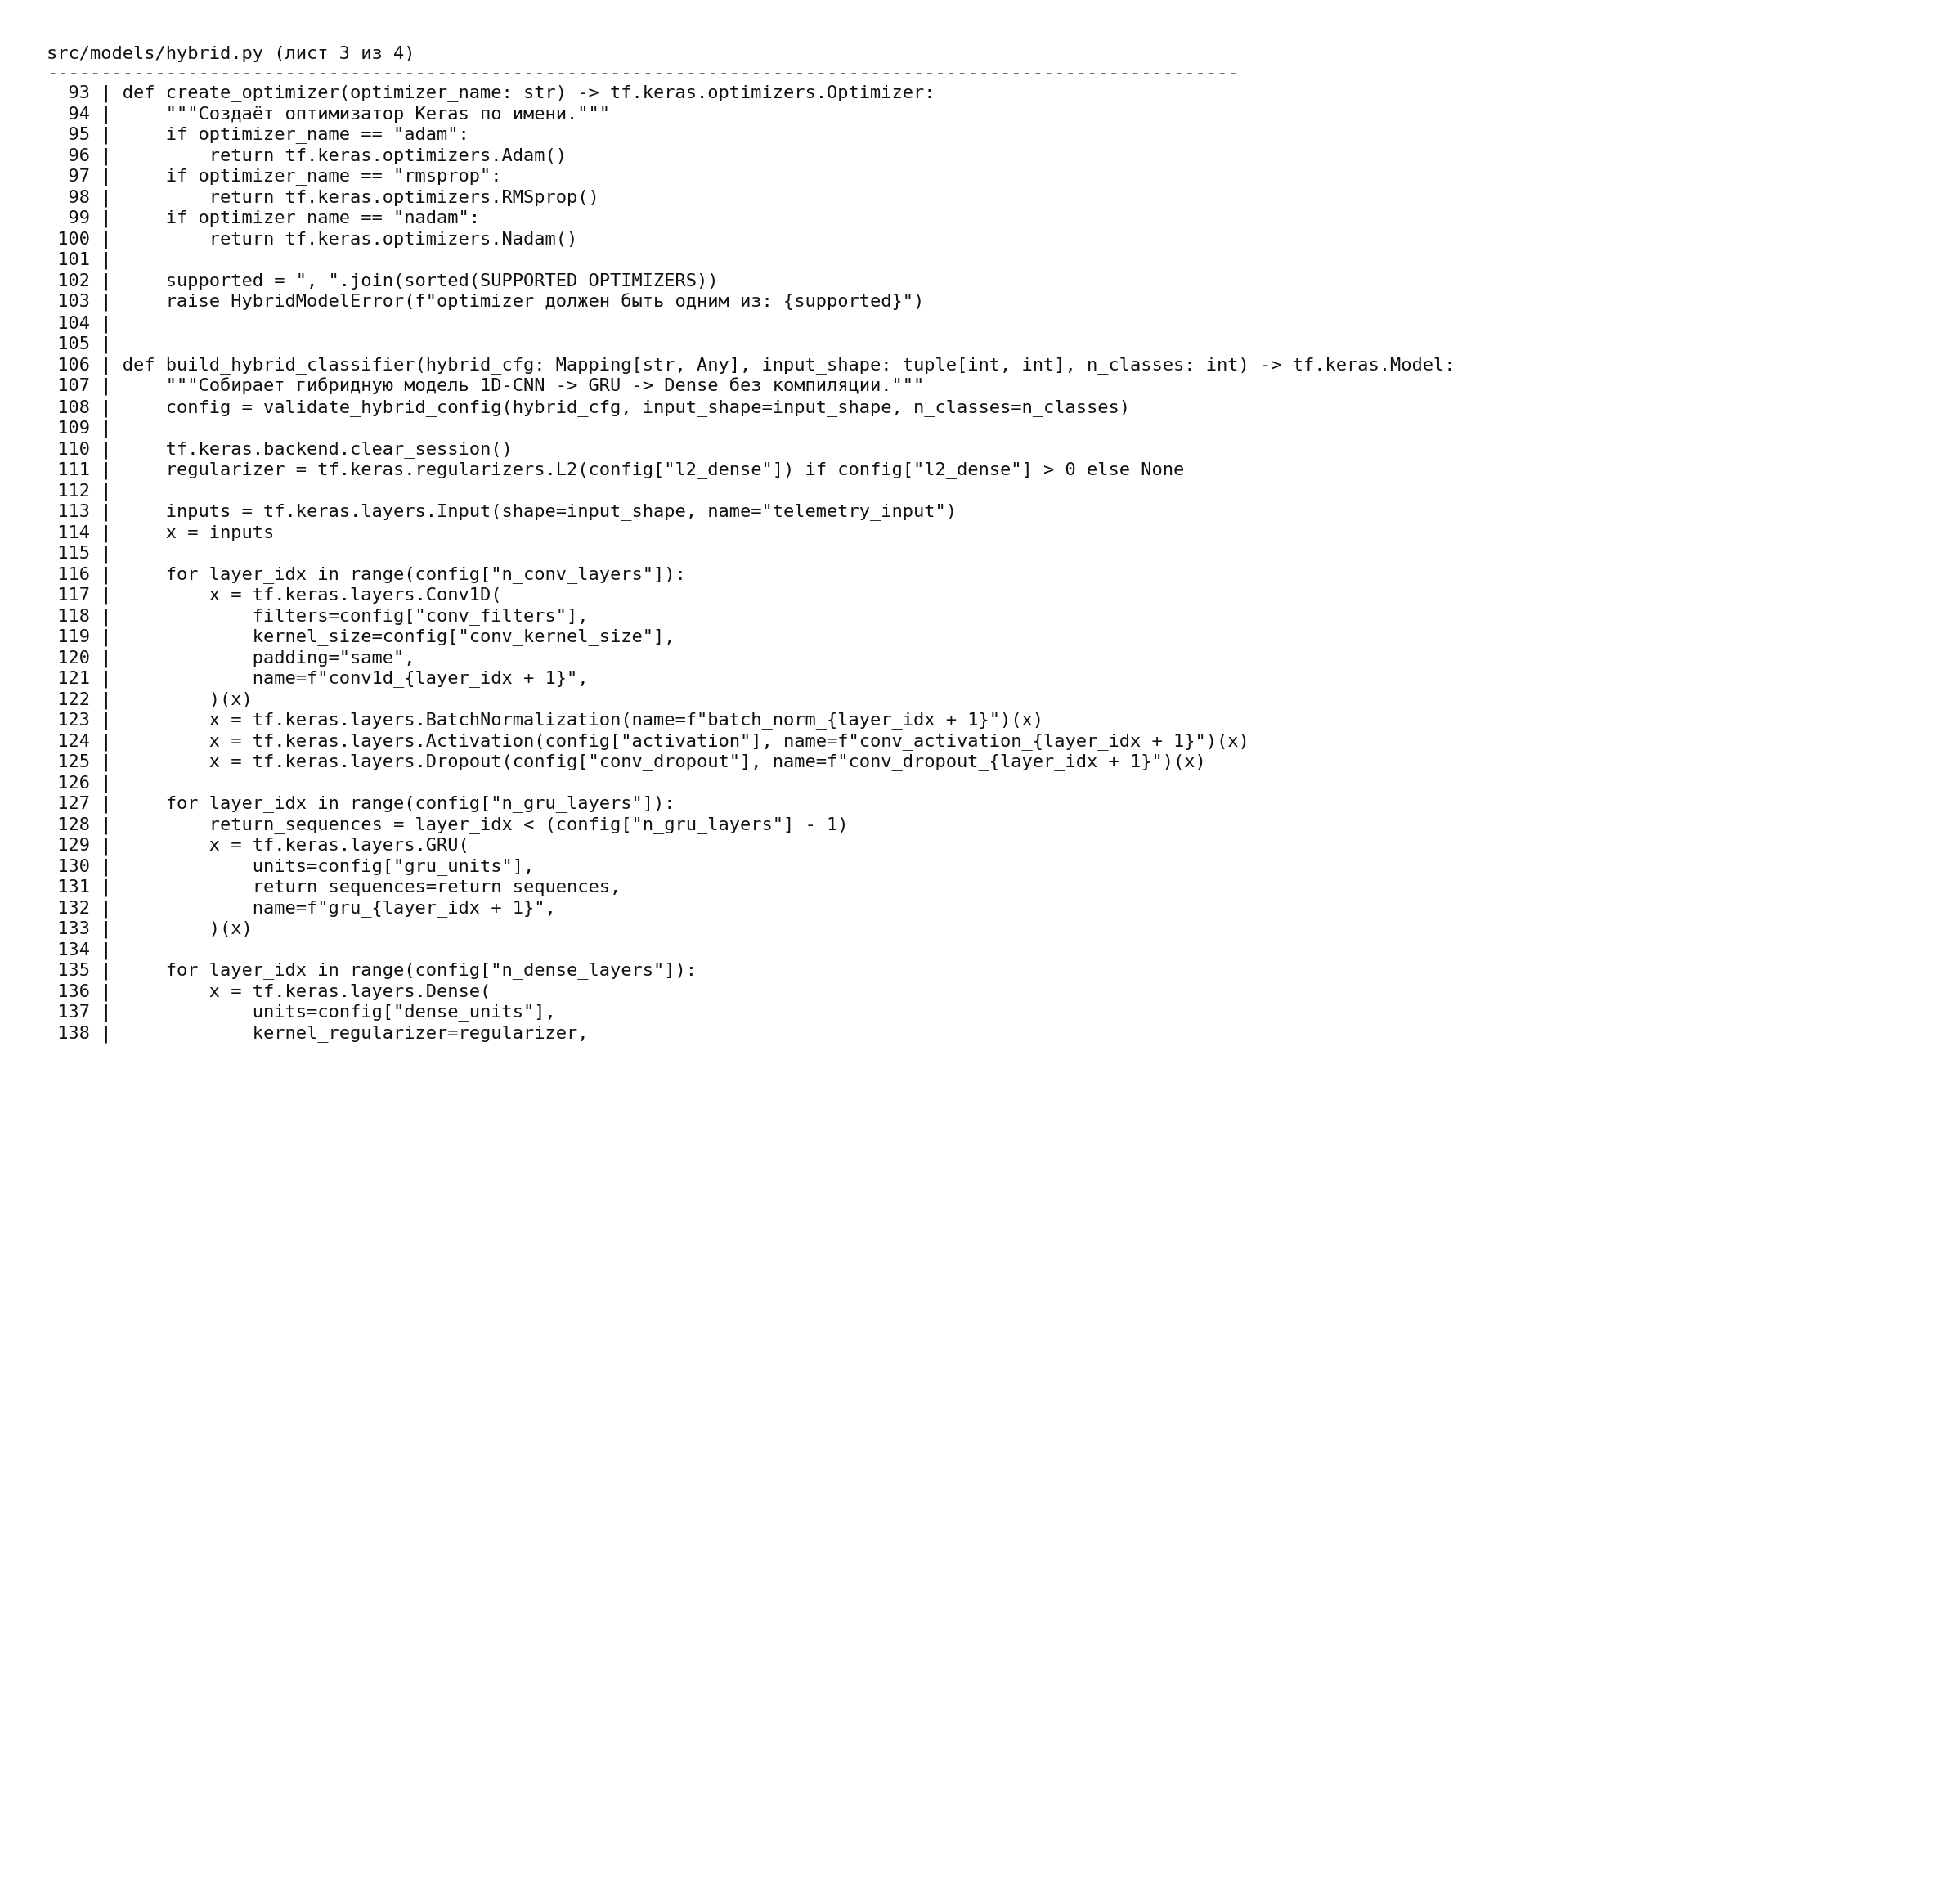
\includegraphics[width=\textwidth]{figures/appendix_hybrid_p03.png}
\caption{Листинг файла src/models/hybrid.py, лист 3}
\end{figure}
\begin{figure}[H]
\centering
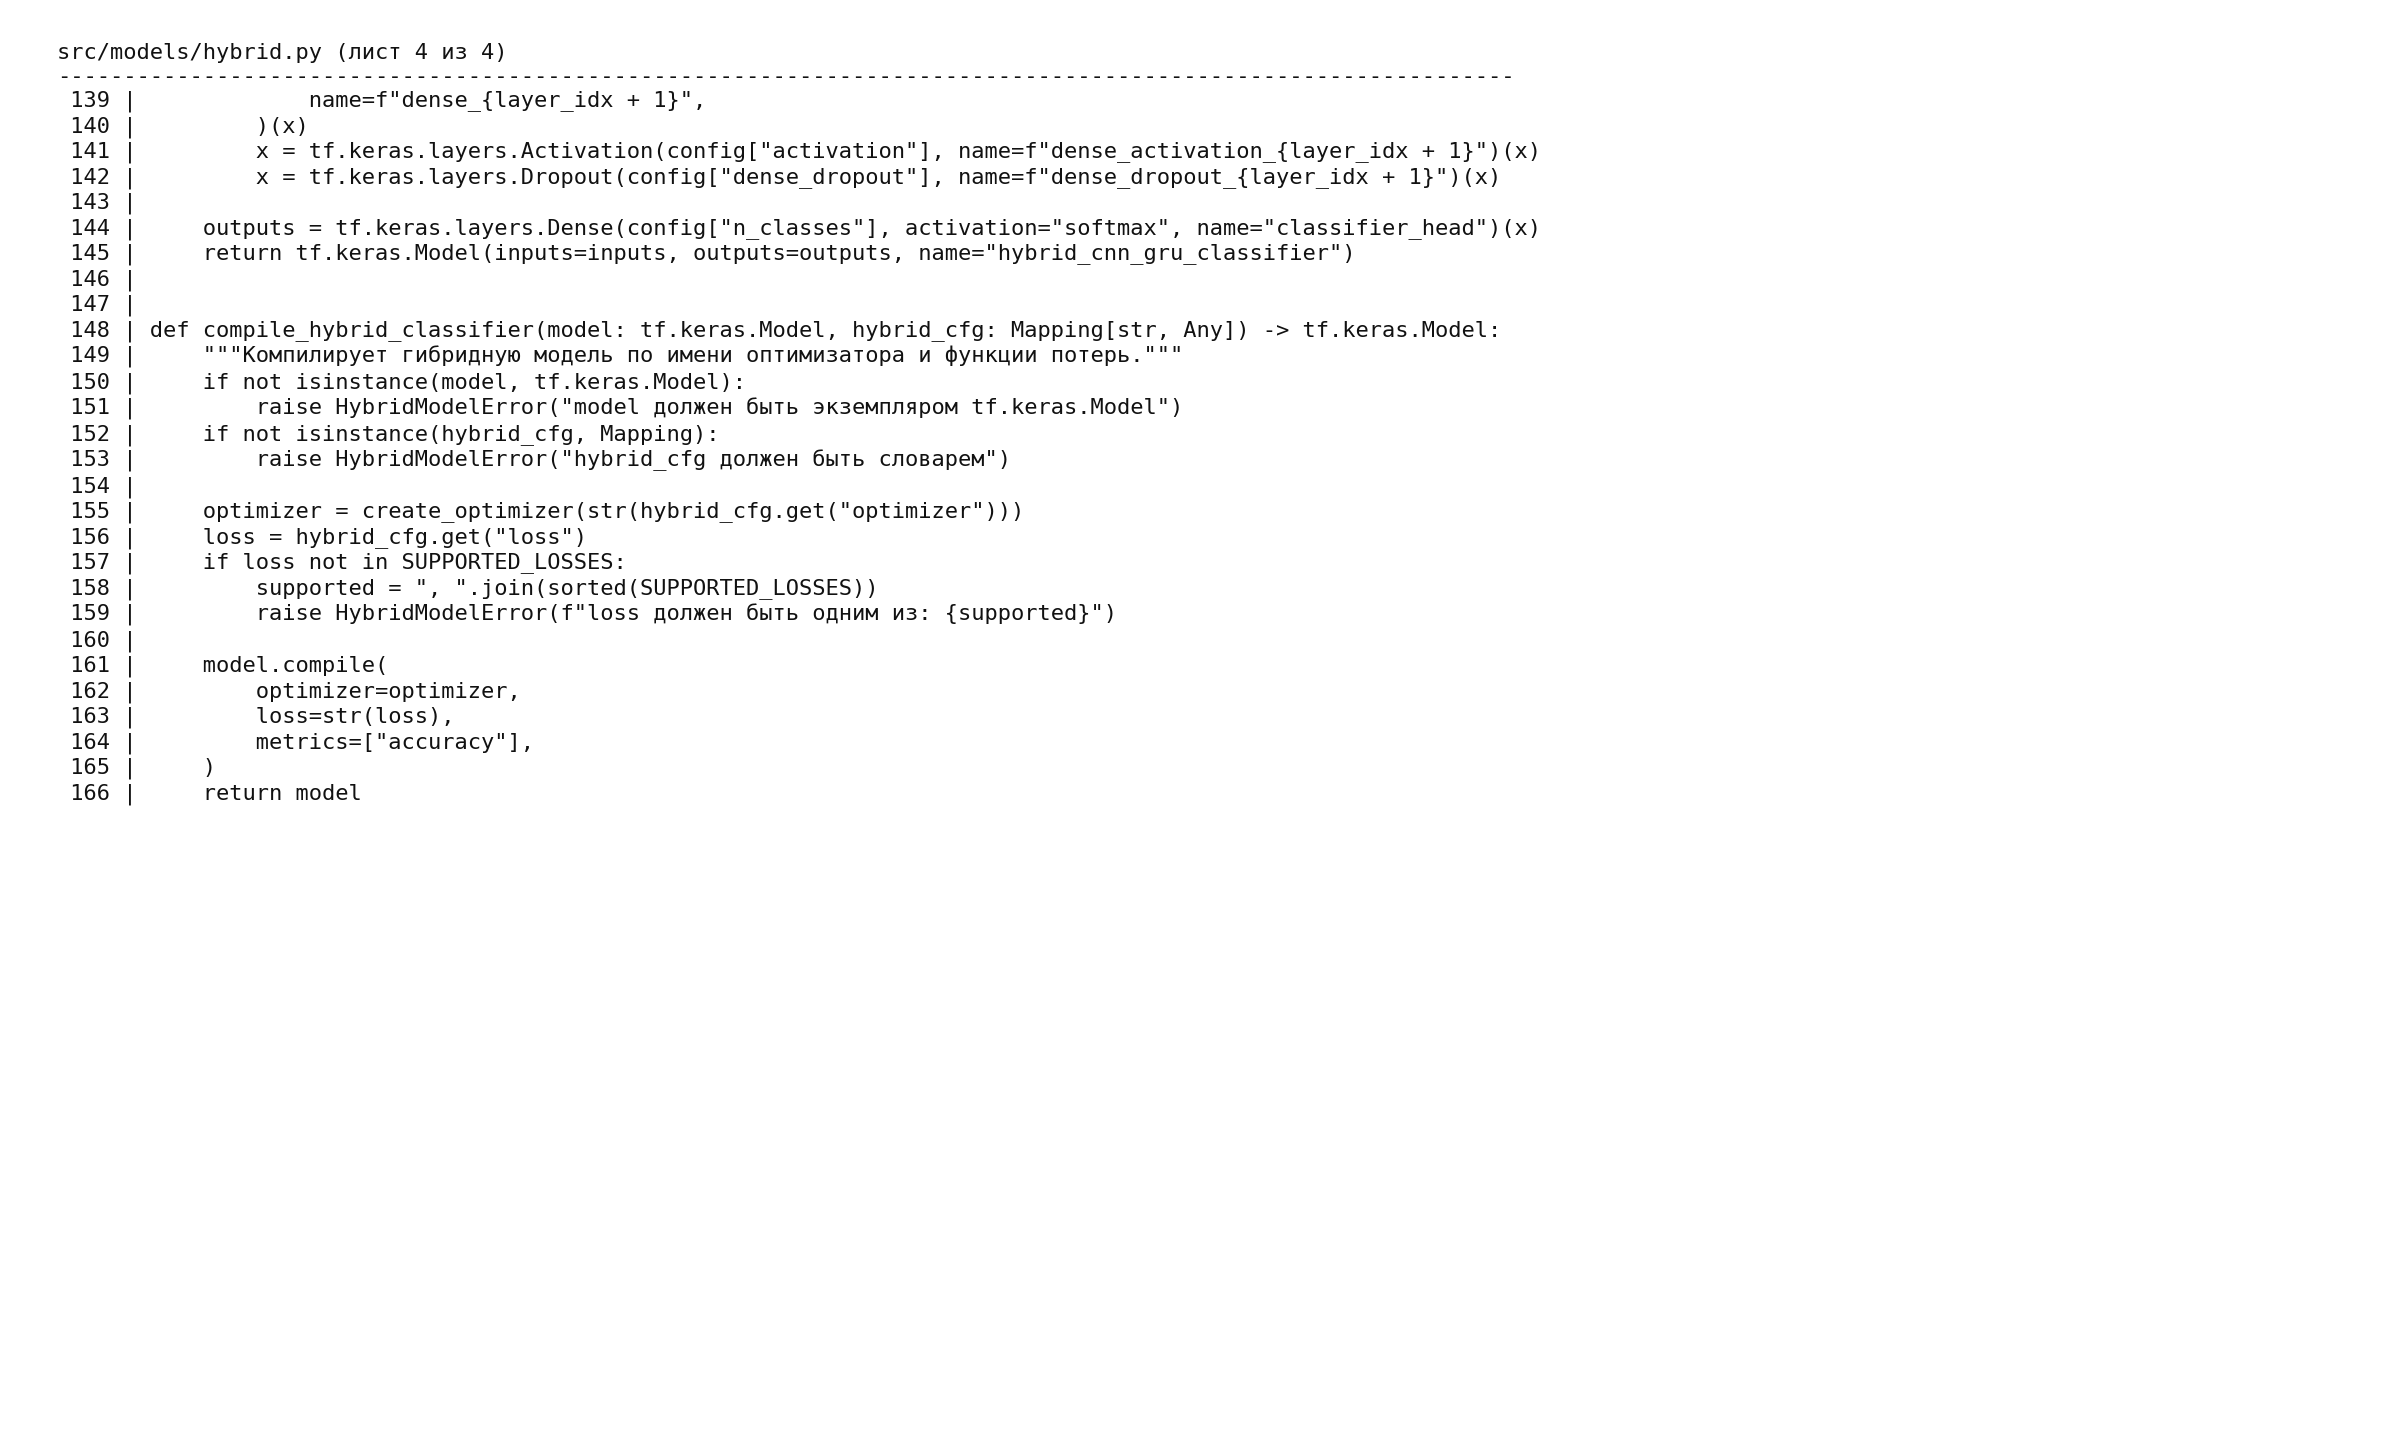
\includegraphics[width=\textwidth]{figures/appendix_hybrid_p04.png}
\caption{Листинг файла src/models/hybrid.py, лист 4}
\end{figure}
\clearpage
\section*{Приложение В. Генетический алгоритм подбора гиперпараметров}
\addcontentsline{toc}{section}{Приложение В. Генетический алгоритм подбора гиперпараметров}
\noindent\textbf{Файл:} \path{src/training/ga_search.py}
\par\vspace{0.4cm}
\begin{figure}[H]
\centering
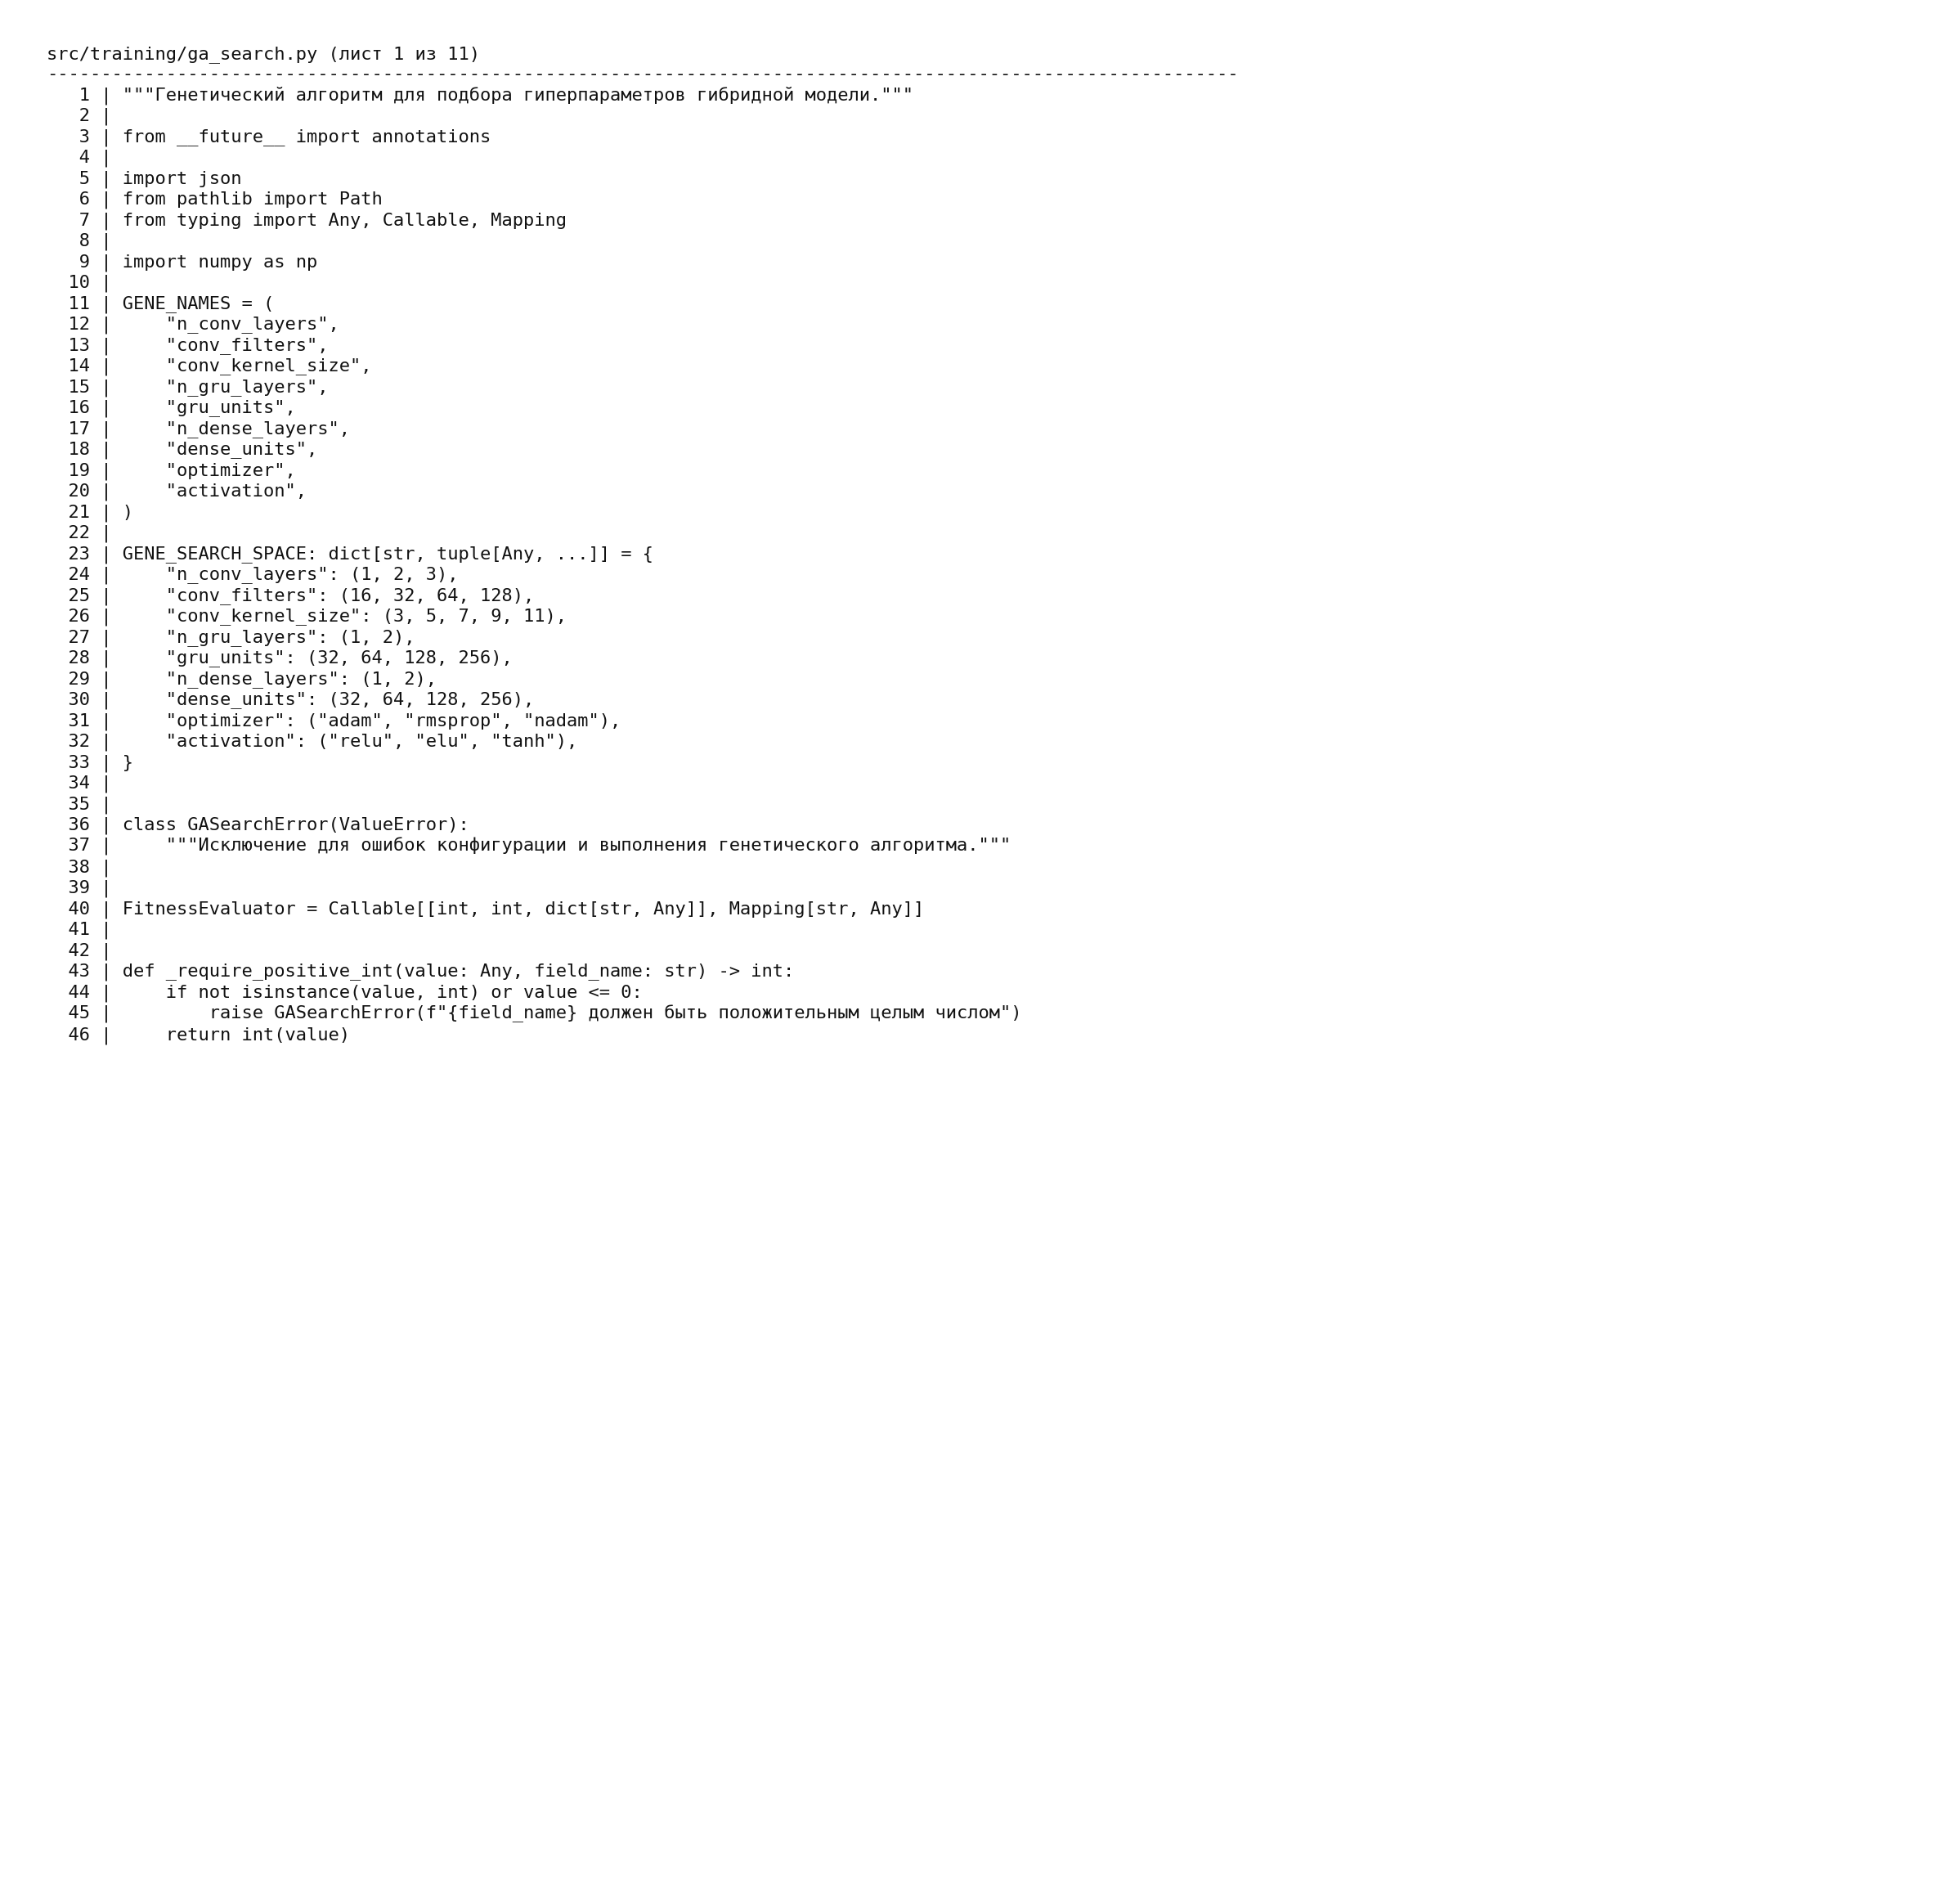
\includegraphics[width=\textwidth]{figures/appendix_ga_p01.png}
\caption{Листинг файла src/training/ga\_search.py, лист 1}
\end{figure}
\begin{figure}[H]
\centering
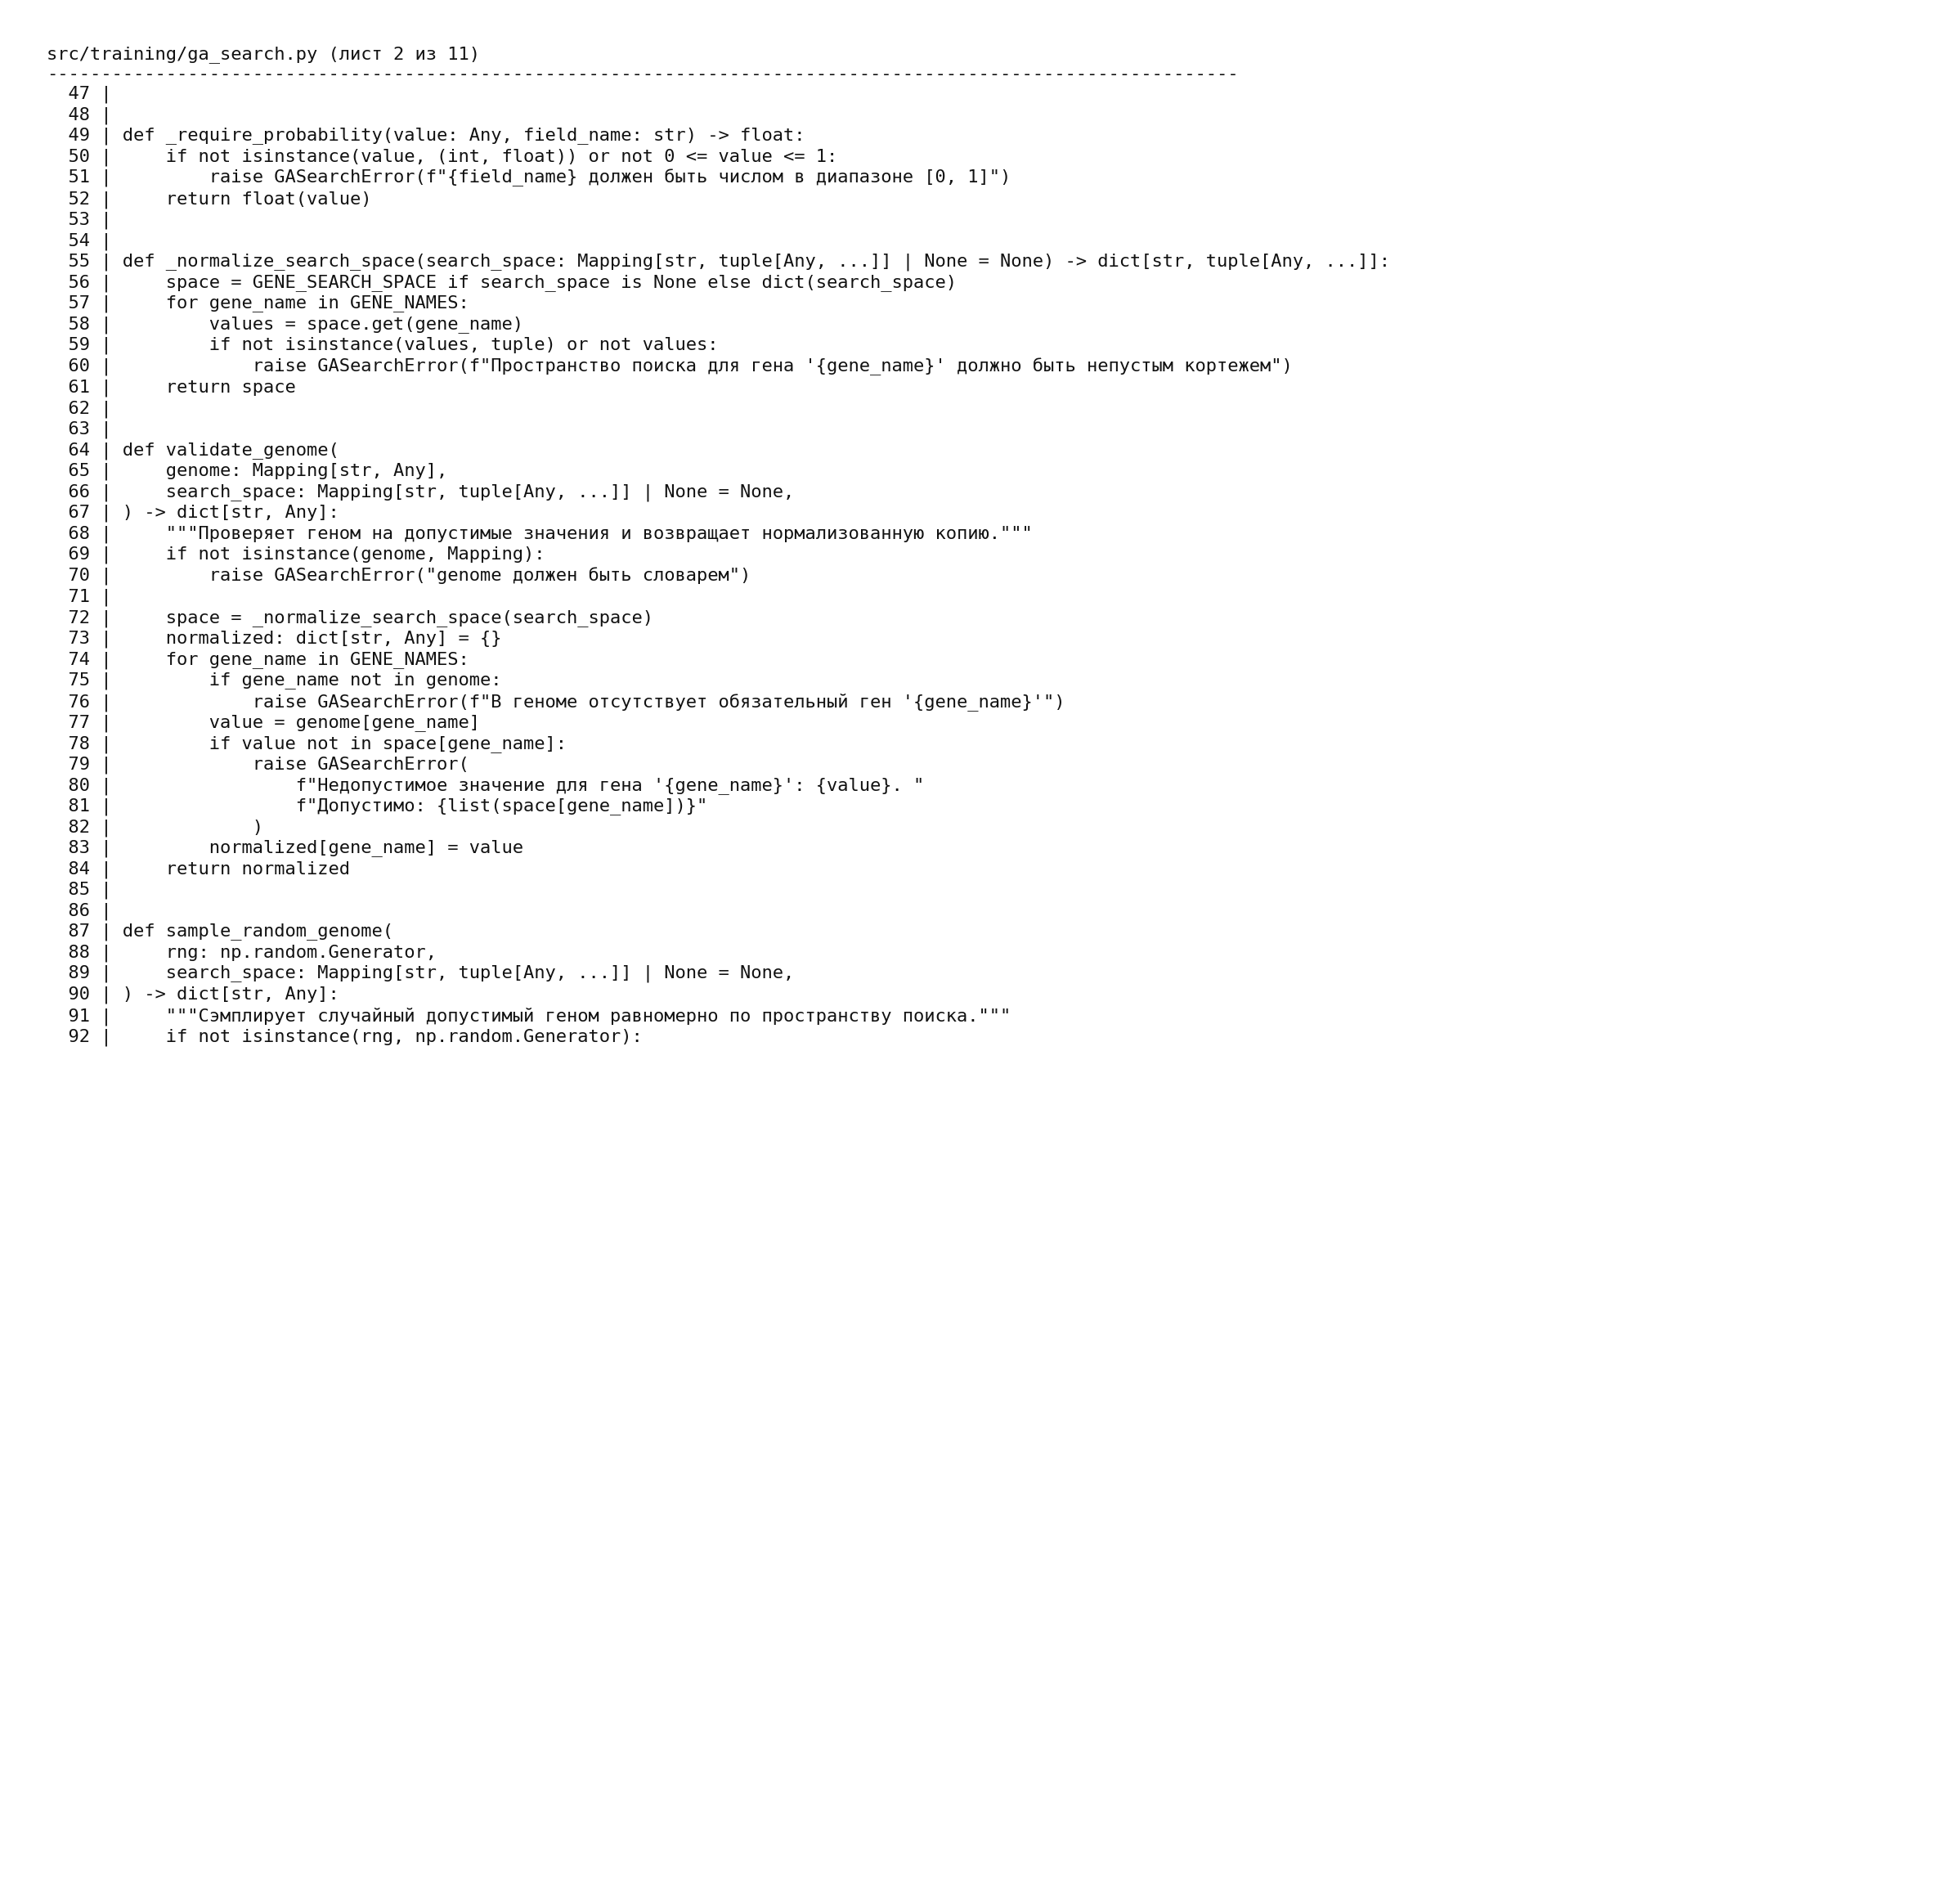
\includegraphics[width=\textwidth]{figures/appendix_ga_p02.png}
\caption{Листинг файла src/training/ga\_search.py, лист 2}
\end{figure}
\begin{figure}[H]
\centering
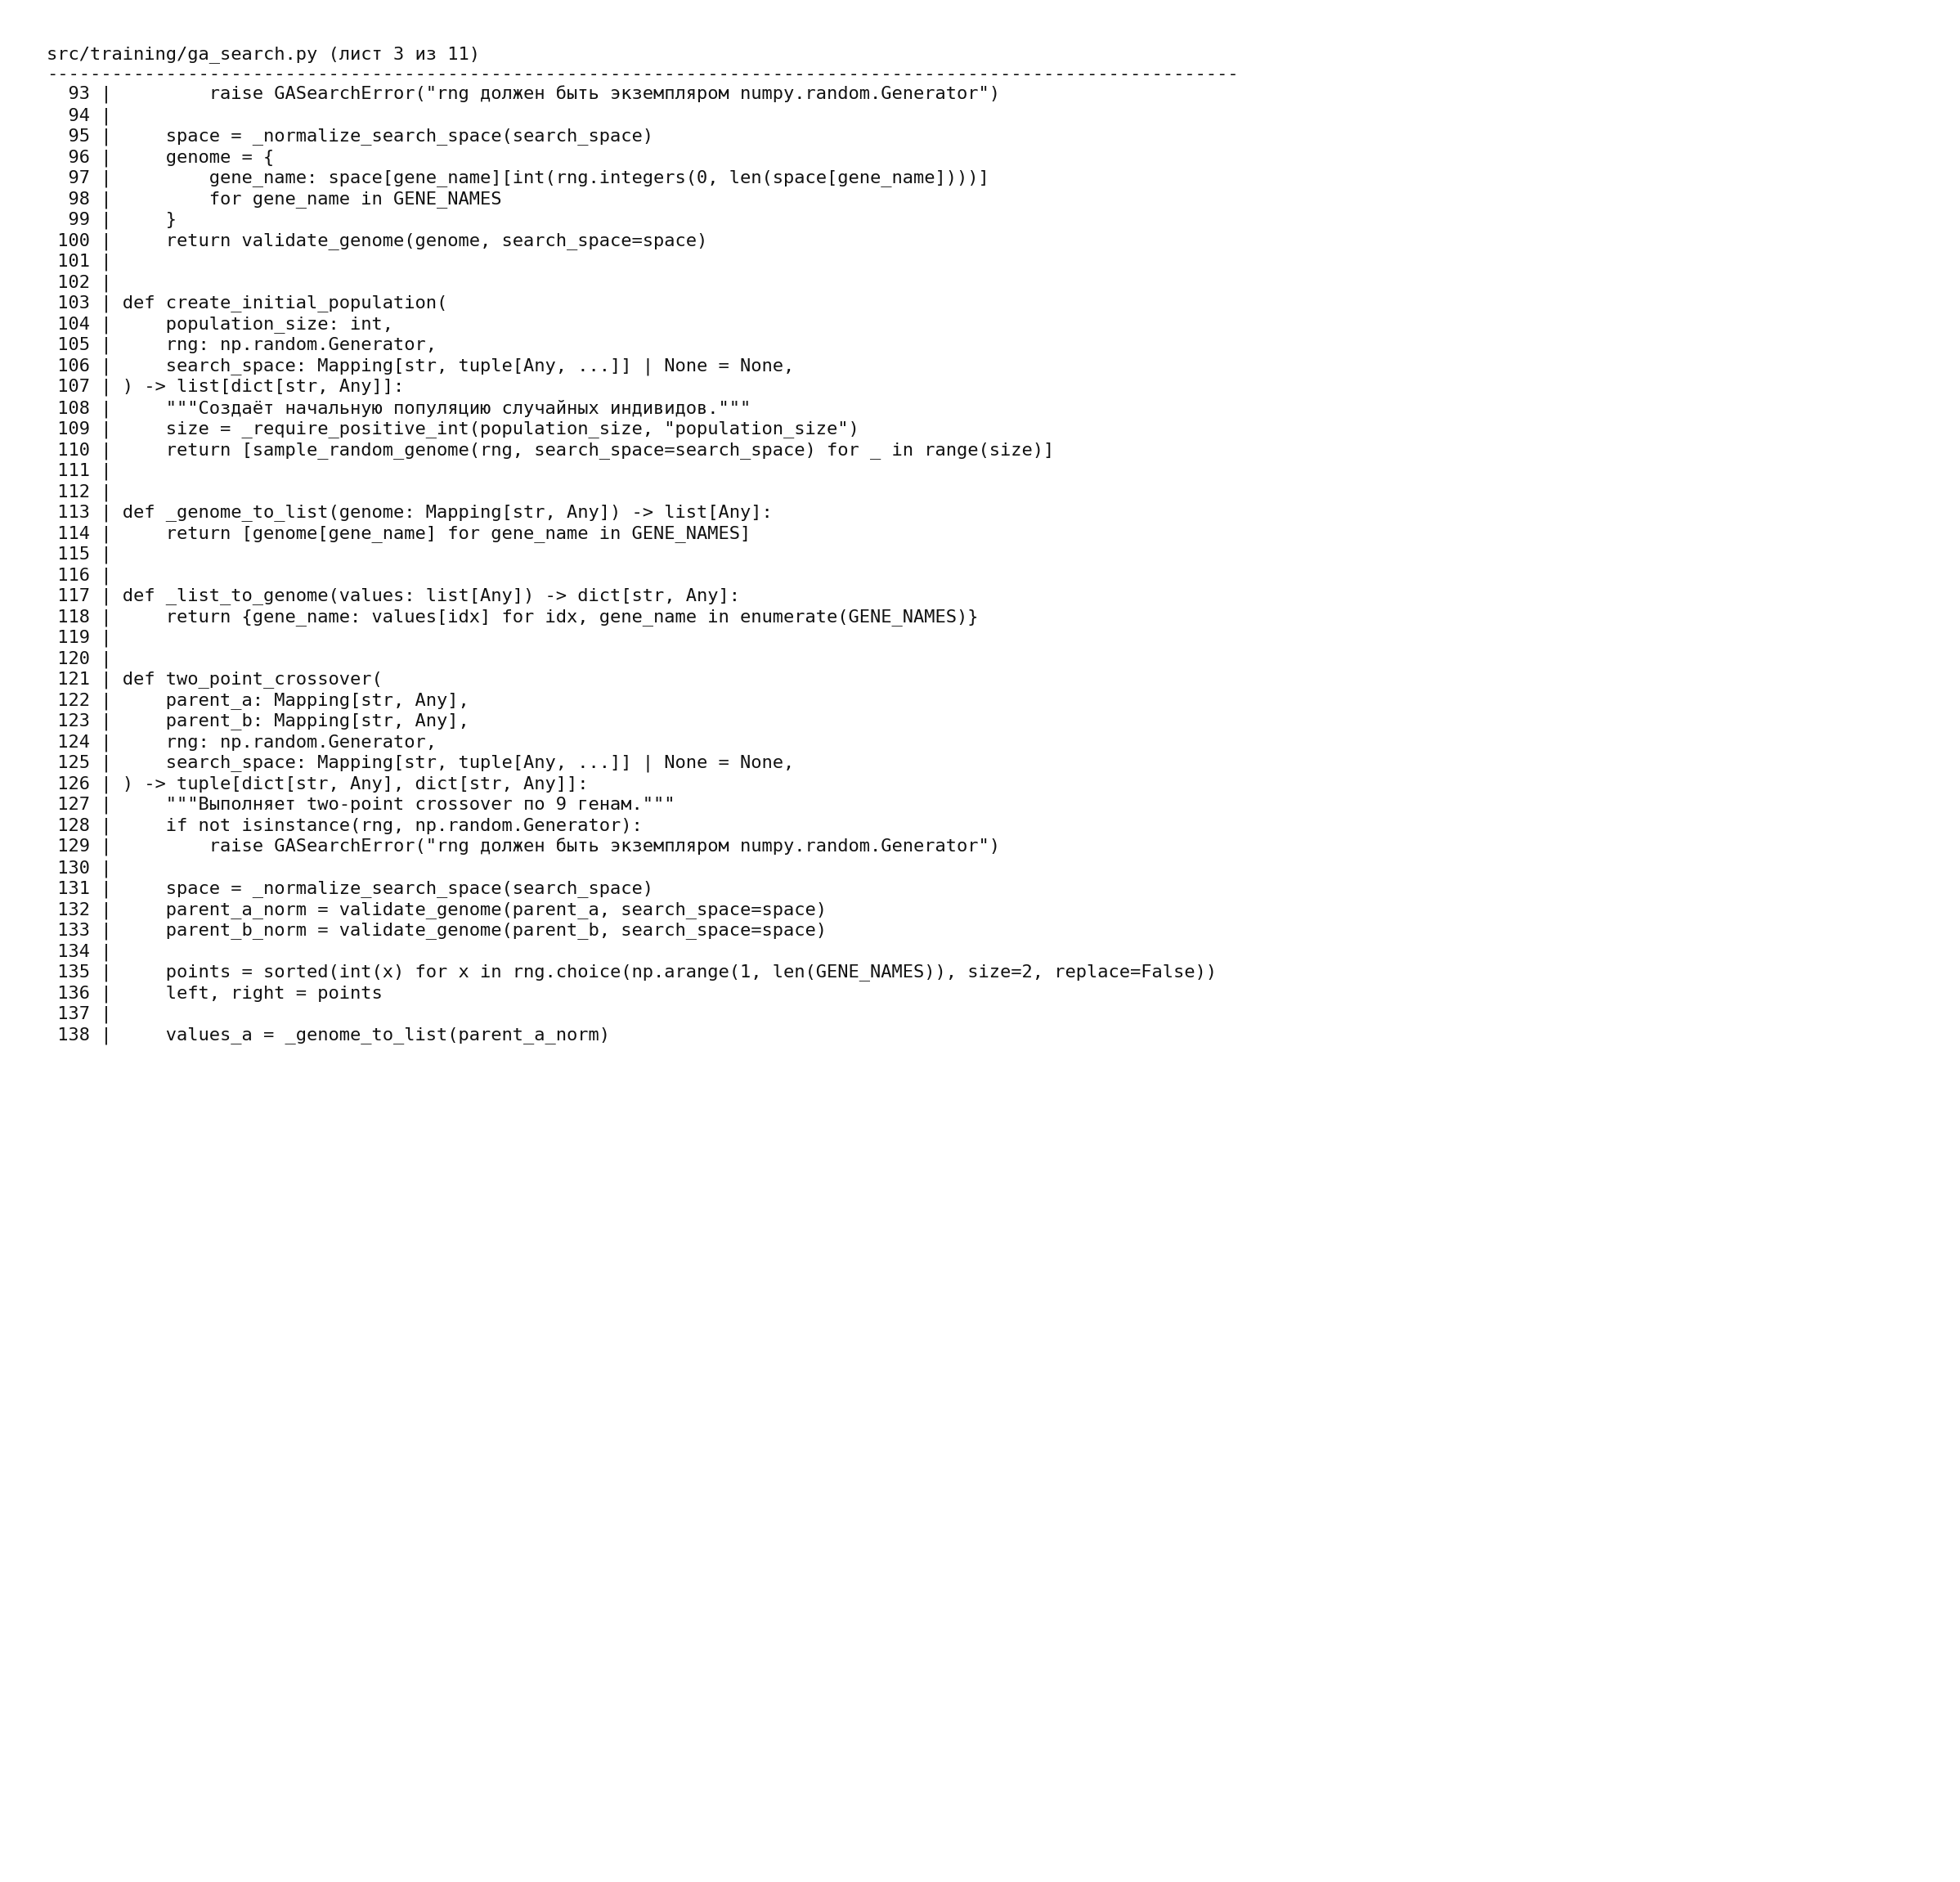
\includegraphics[width=\textwidth]{figures/appendix_ga_p03.png}
\caption{Листинг файла src/training/ga\_search.py, лист 3}
\end{figure}
\begin{figure}[H]
\centering
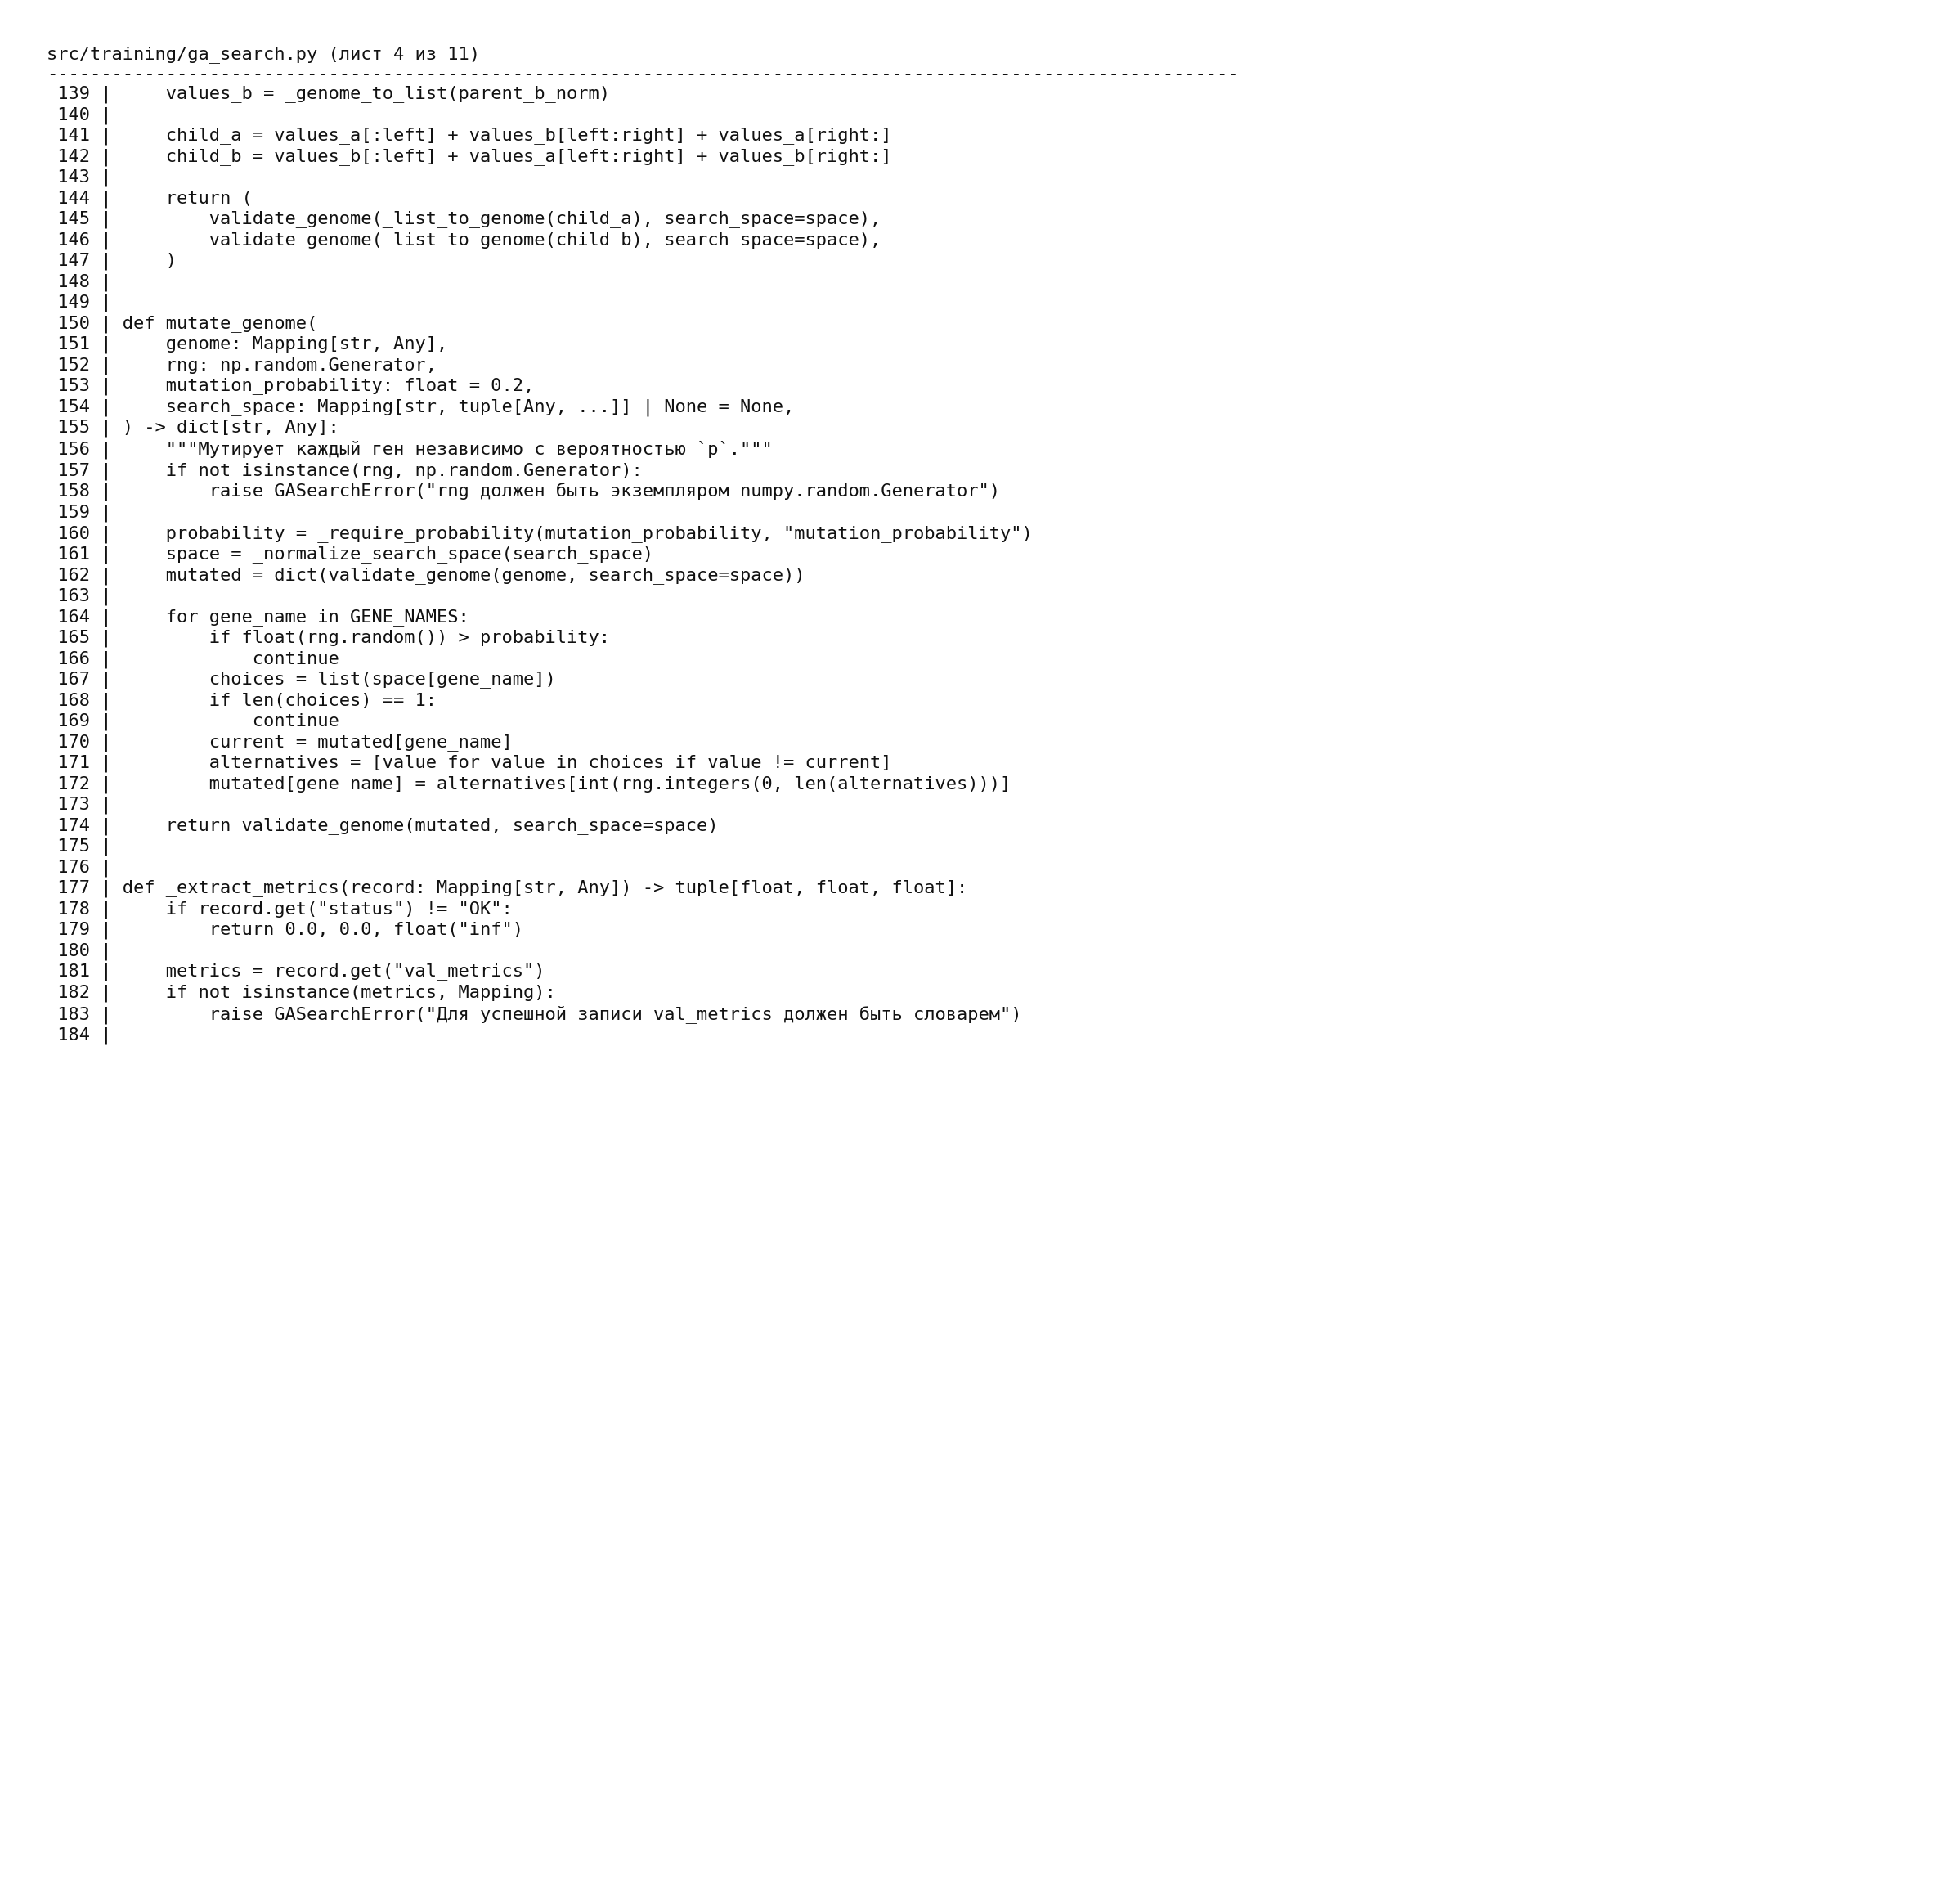
\includegraphics[width=\textwidth]{figures/appendix_ga_p04.png}
\caption{Листинг файла src/training/ga\_search.py, лист 4}
\end{figure}
\begin{figure}[H]
\centering
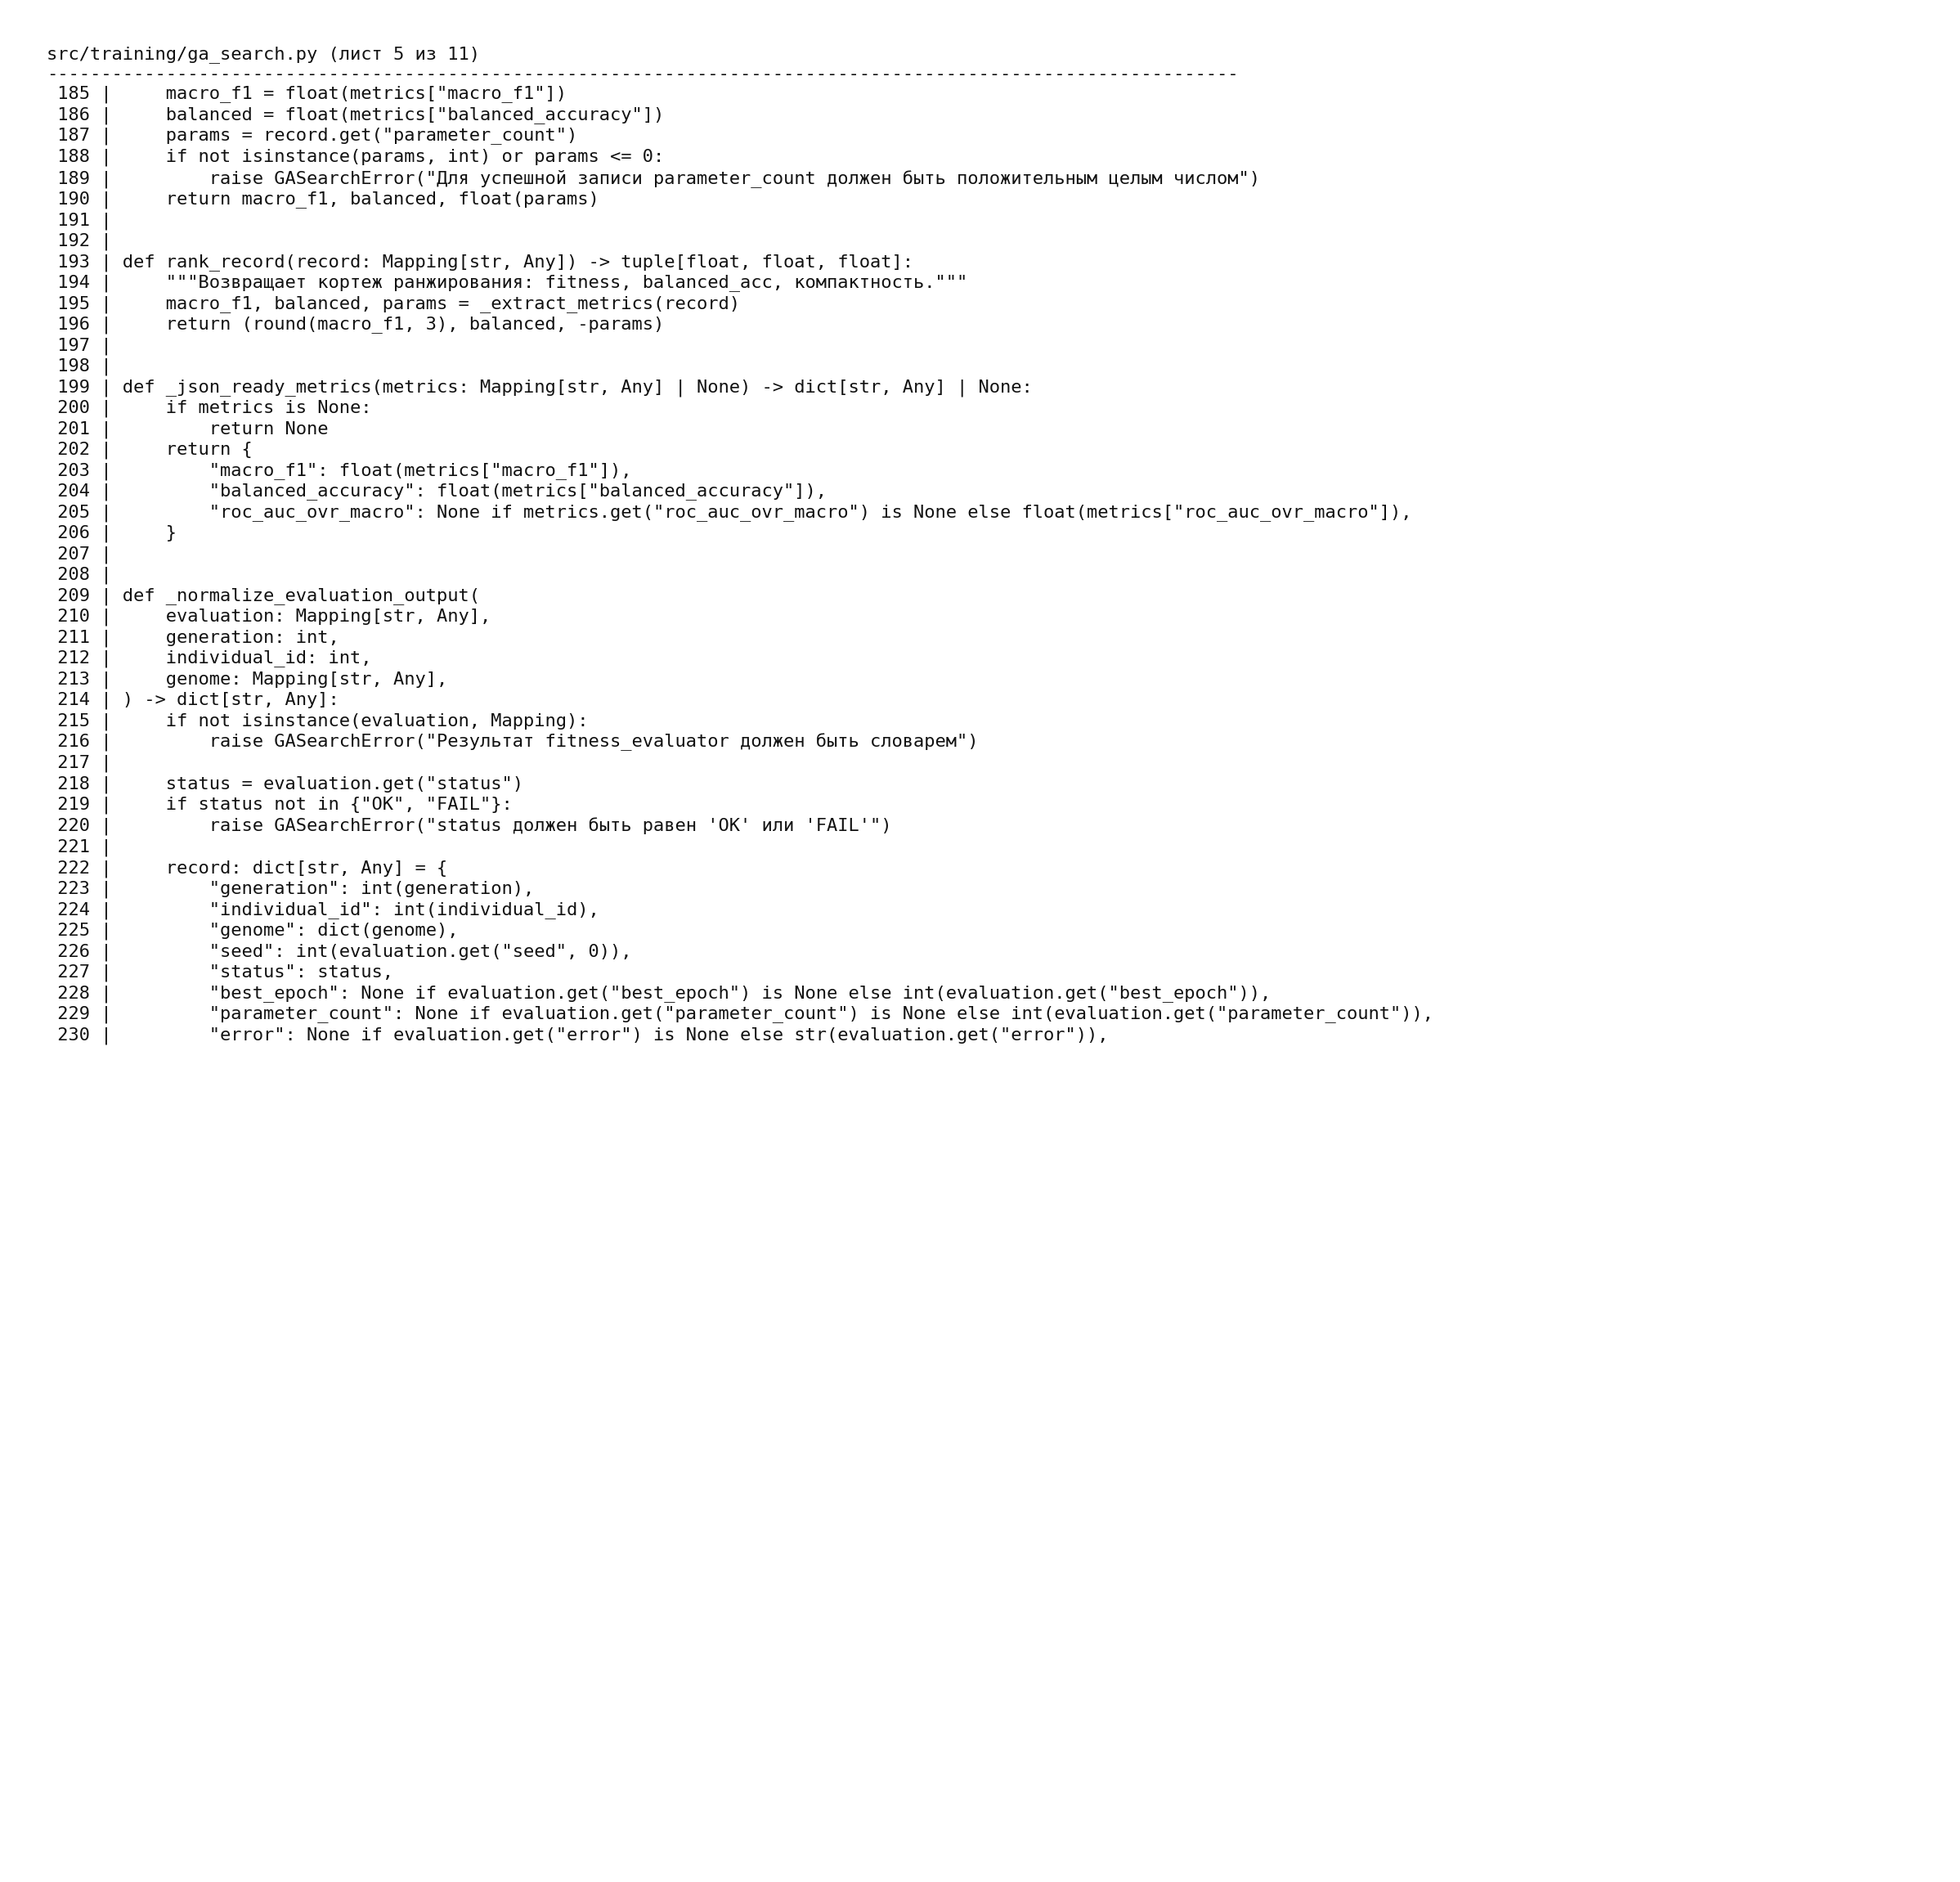
\includegraphics[width=\textwidth]{figures/appendix_ga_p05.png}
\caption{Листинг файла src/training/ga\_search.py, лист 5}
\end{figure}
\begin{figure}[H]
\centering
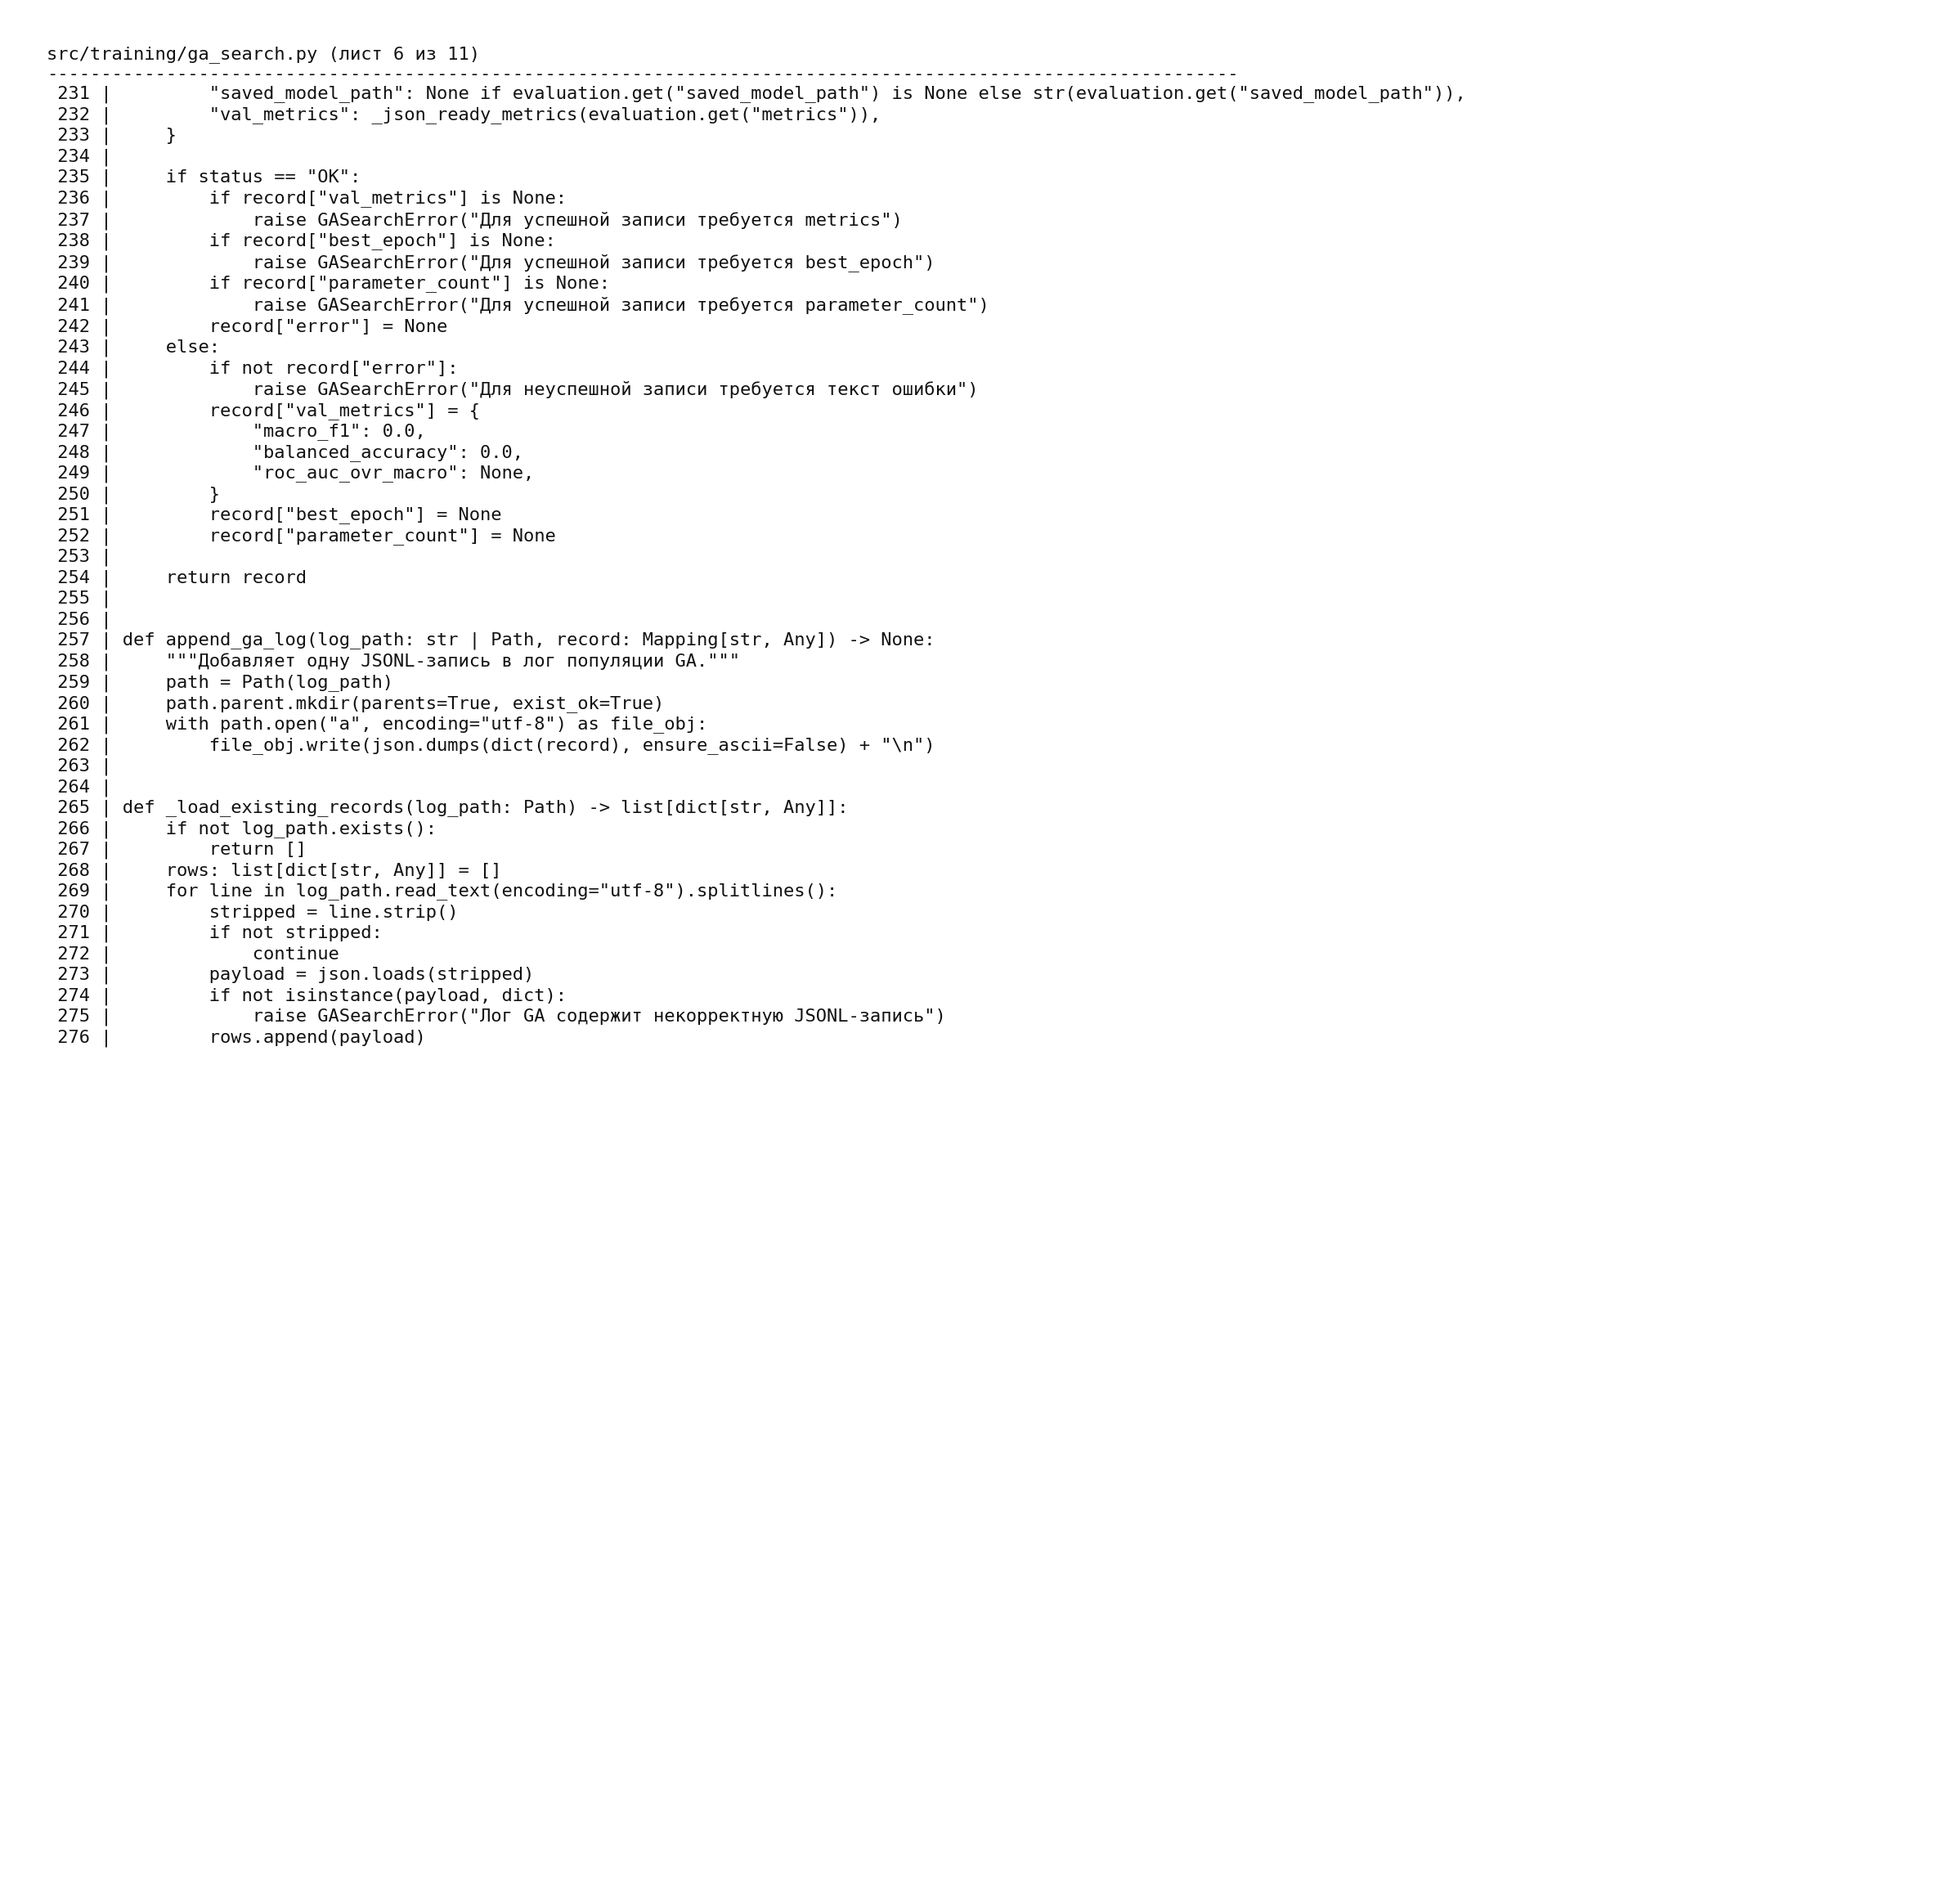
\includegraphics[width=\textwidth]{figures/appendix_ga_p06.png}
\caption{Листинг файла src/training/ga\_search.py, лист 6}
\end{figure}
\begin{figure}[H]
\centering
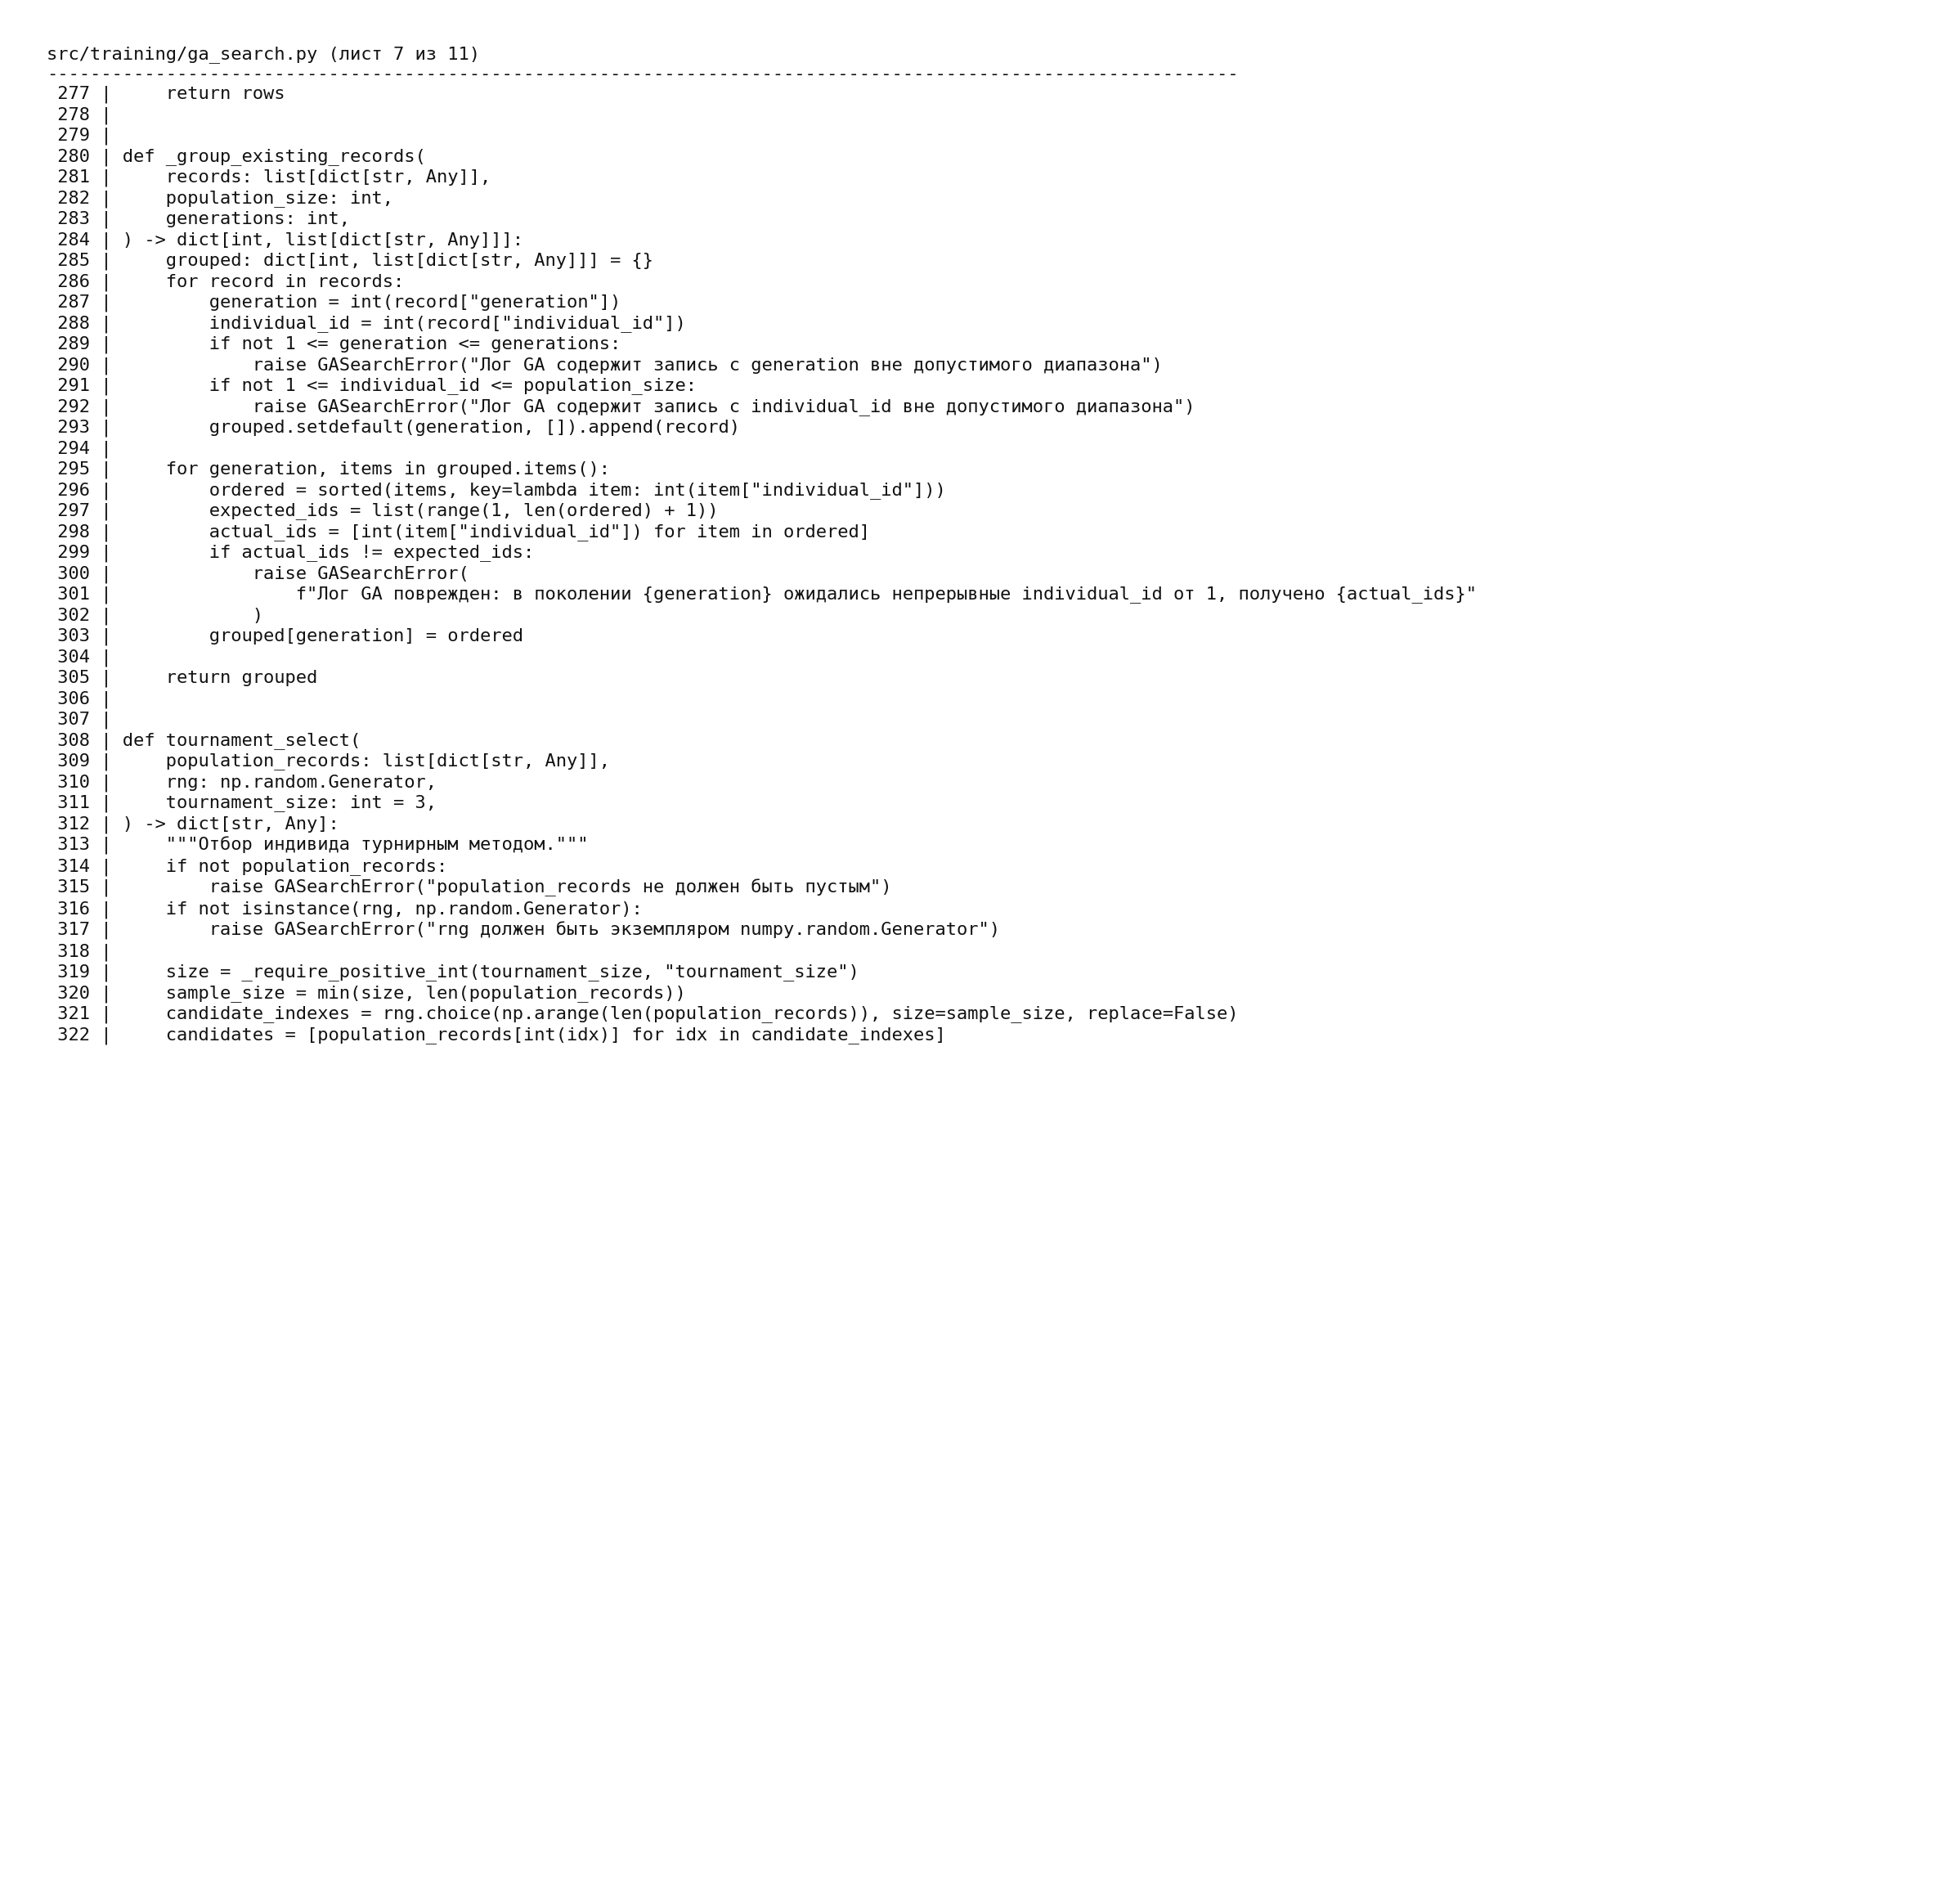
\includegraphics[width=\textwidth]{figures/appendix_ga_p07.png}
\caption{Листинг файла src/training/ga\_search.py, лист 7}
\end{figure}
\begin{figure}[H]
\centering
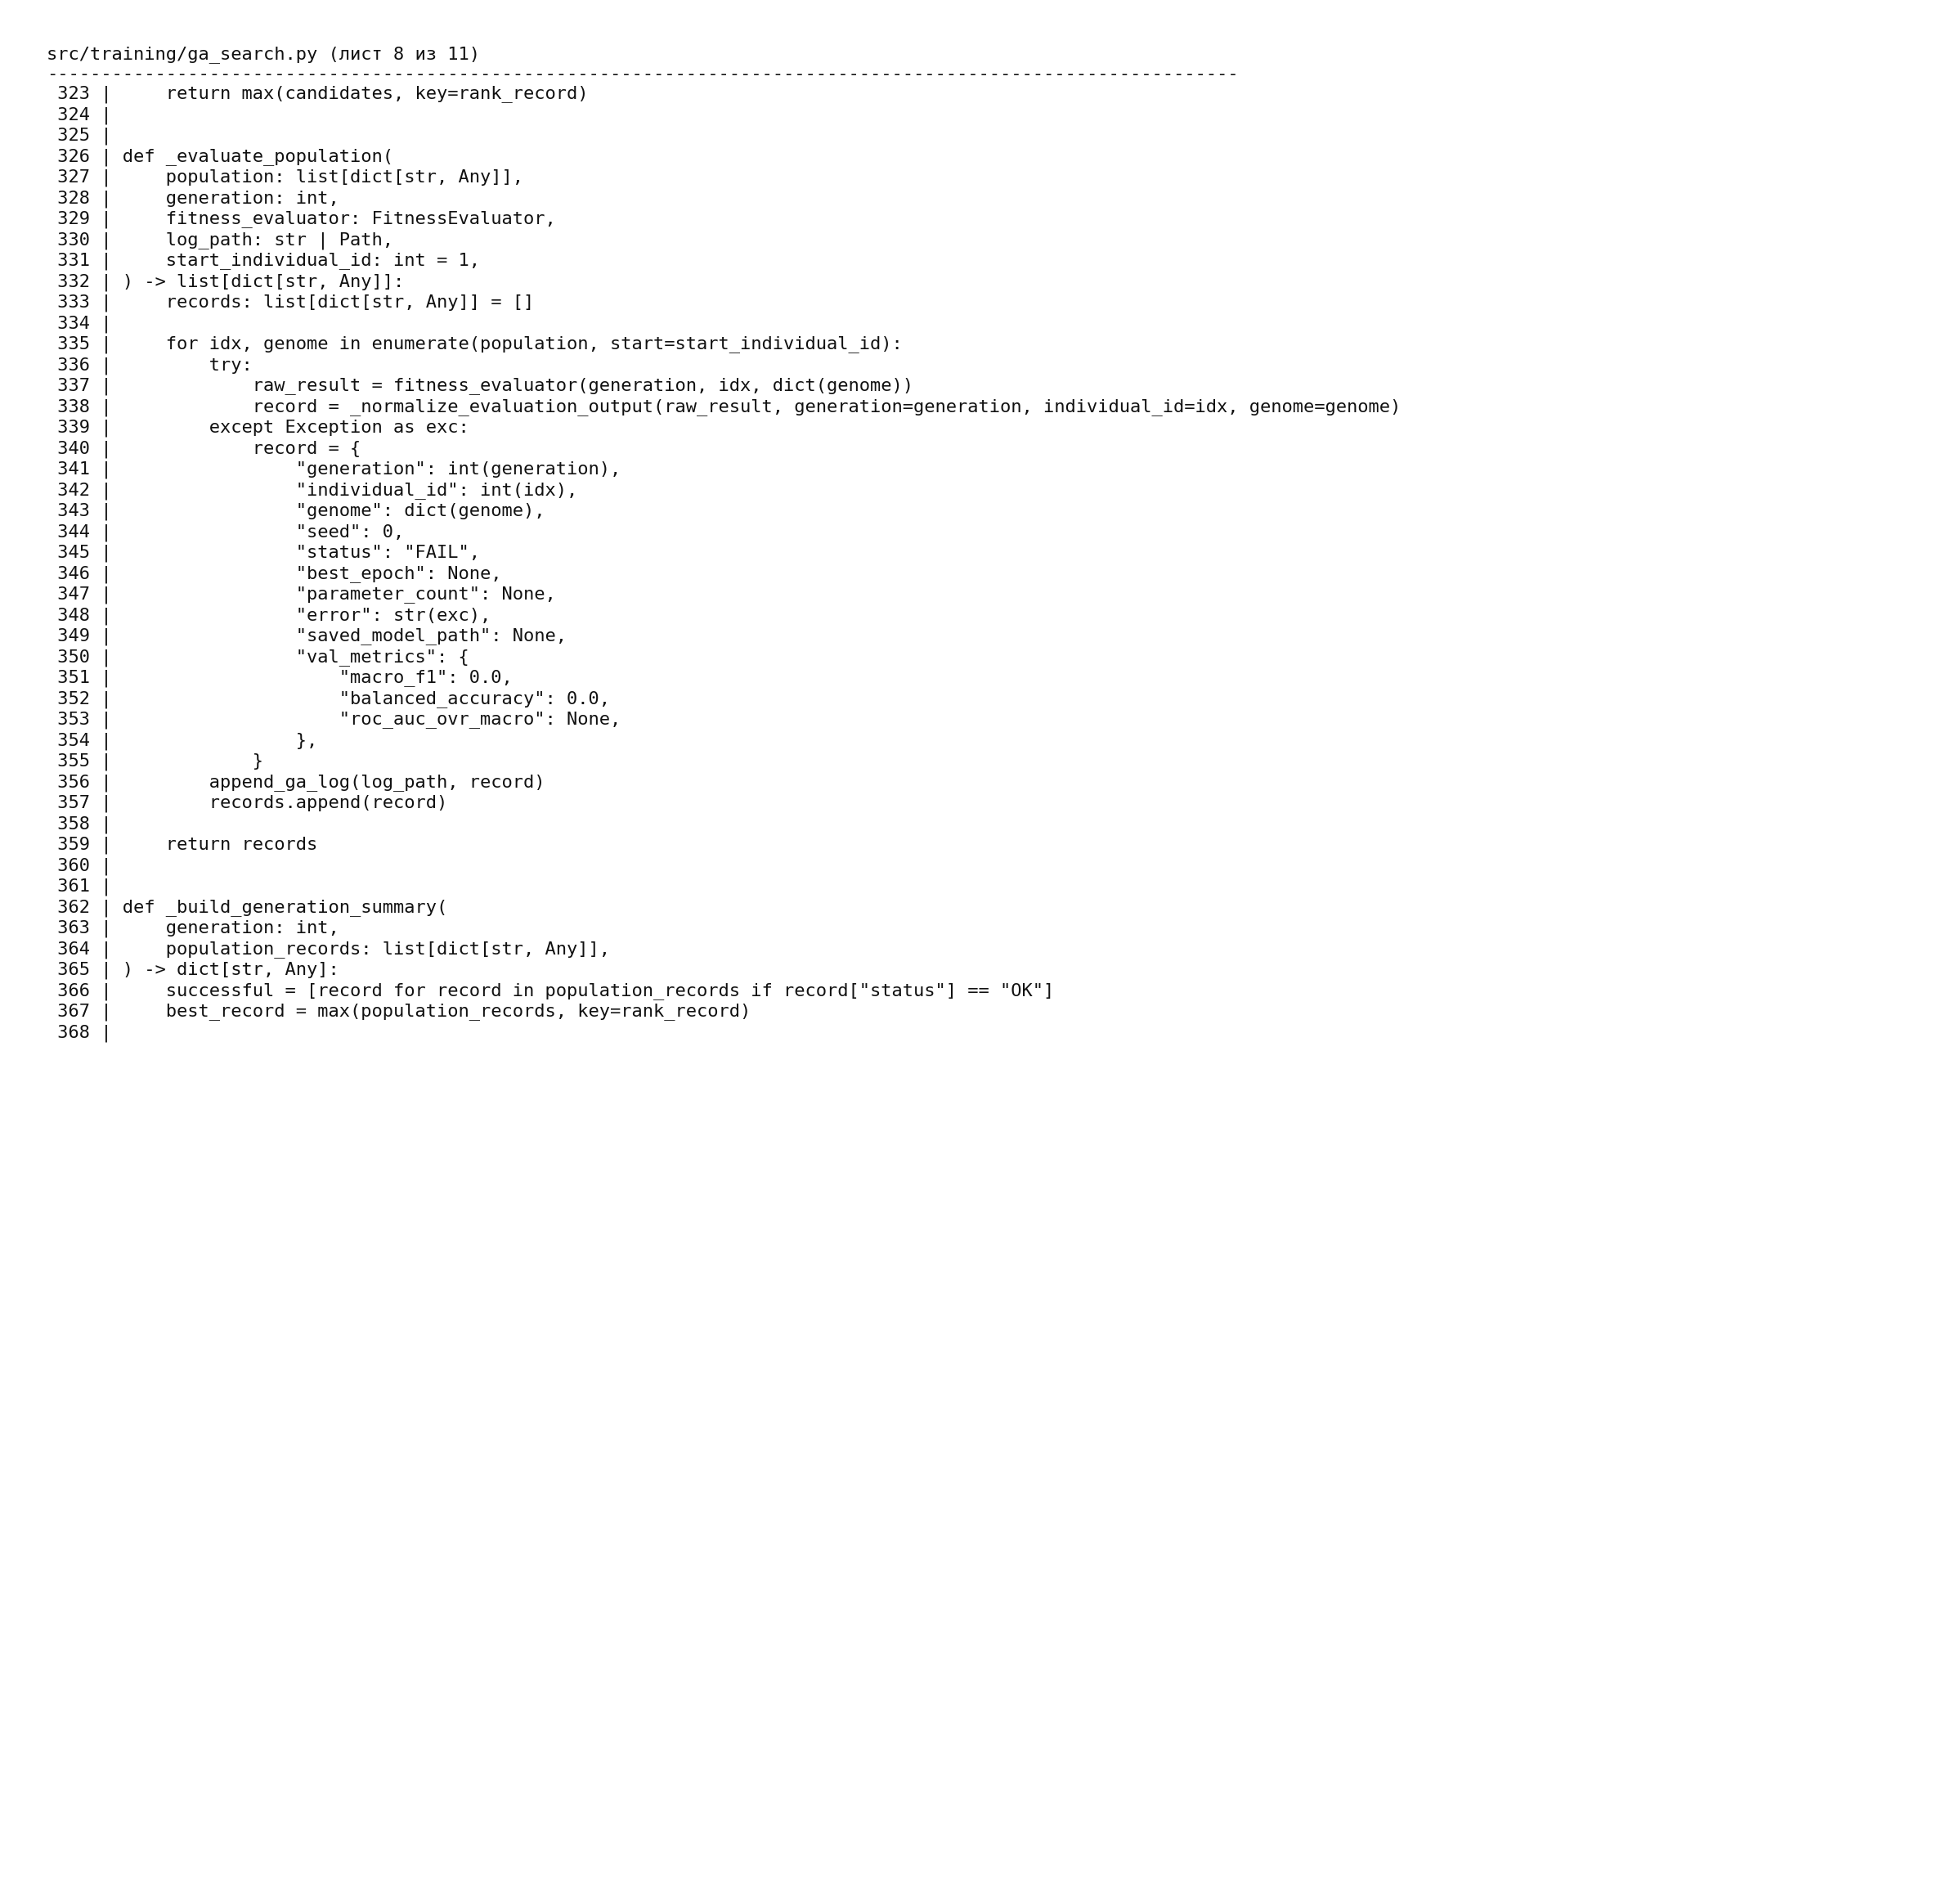
\includegraphics[width=\textwidth]{figures/appendix_ga_p08.png}
\caption{Листинг файла src/training/ga\_search.py, лист 8}
\end{figure}
\begin{figure}[H]
\centering
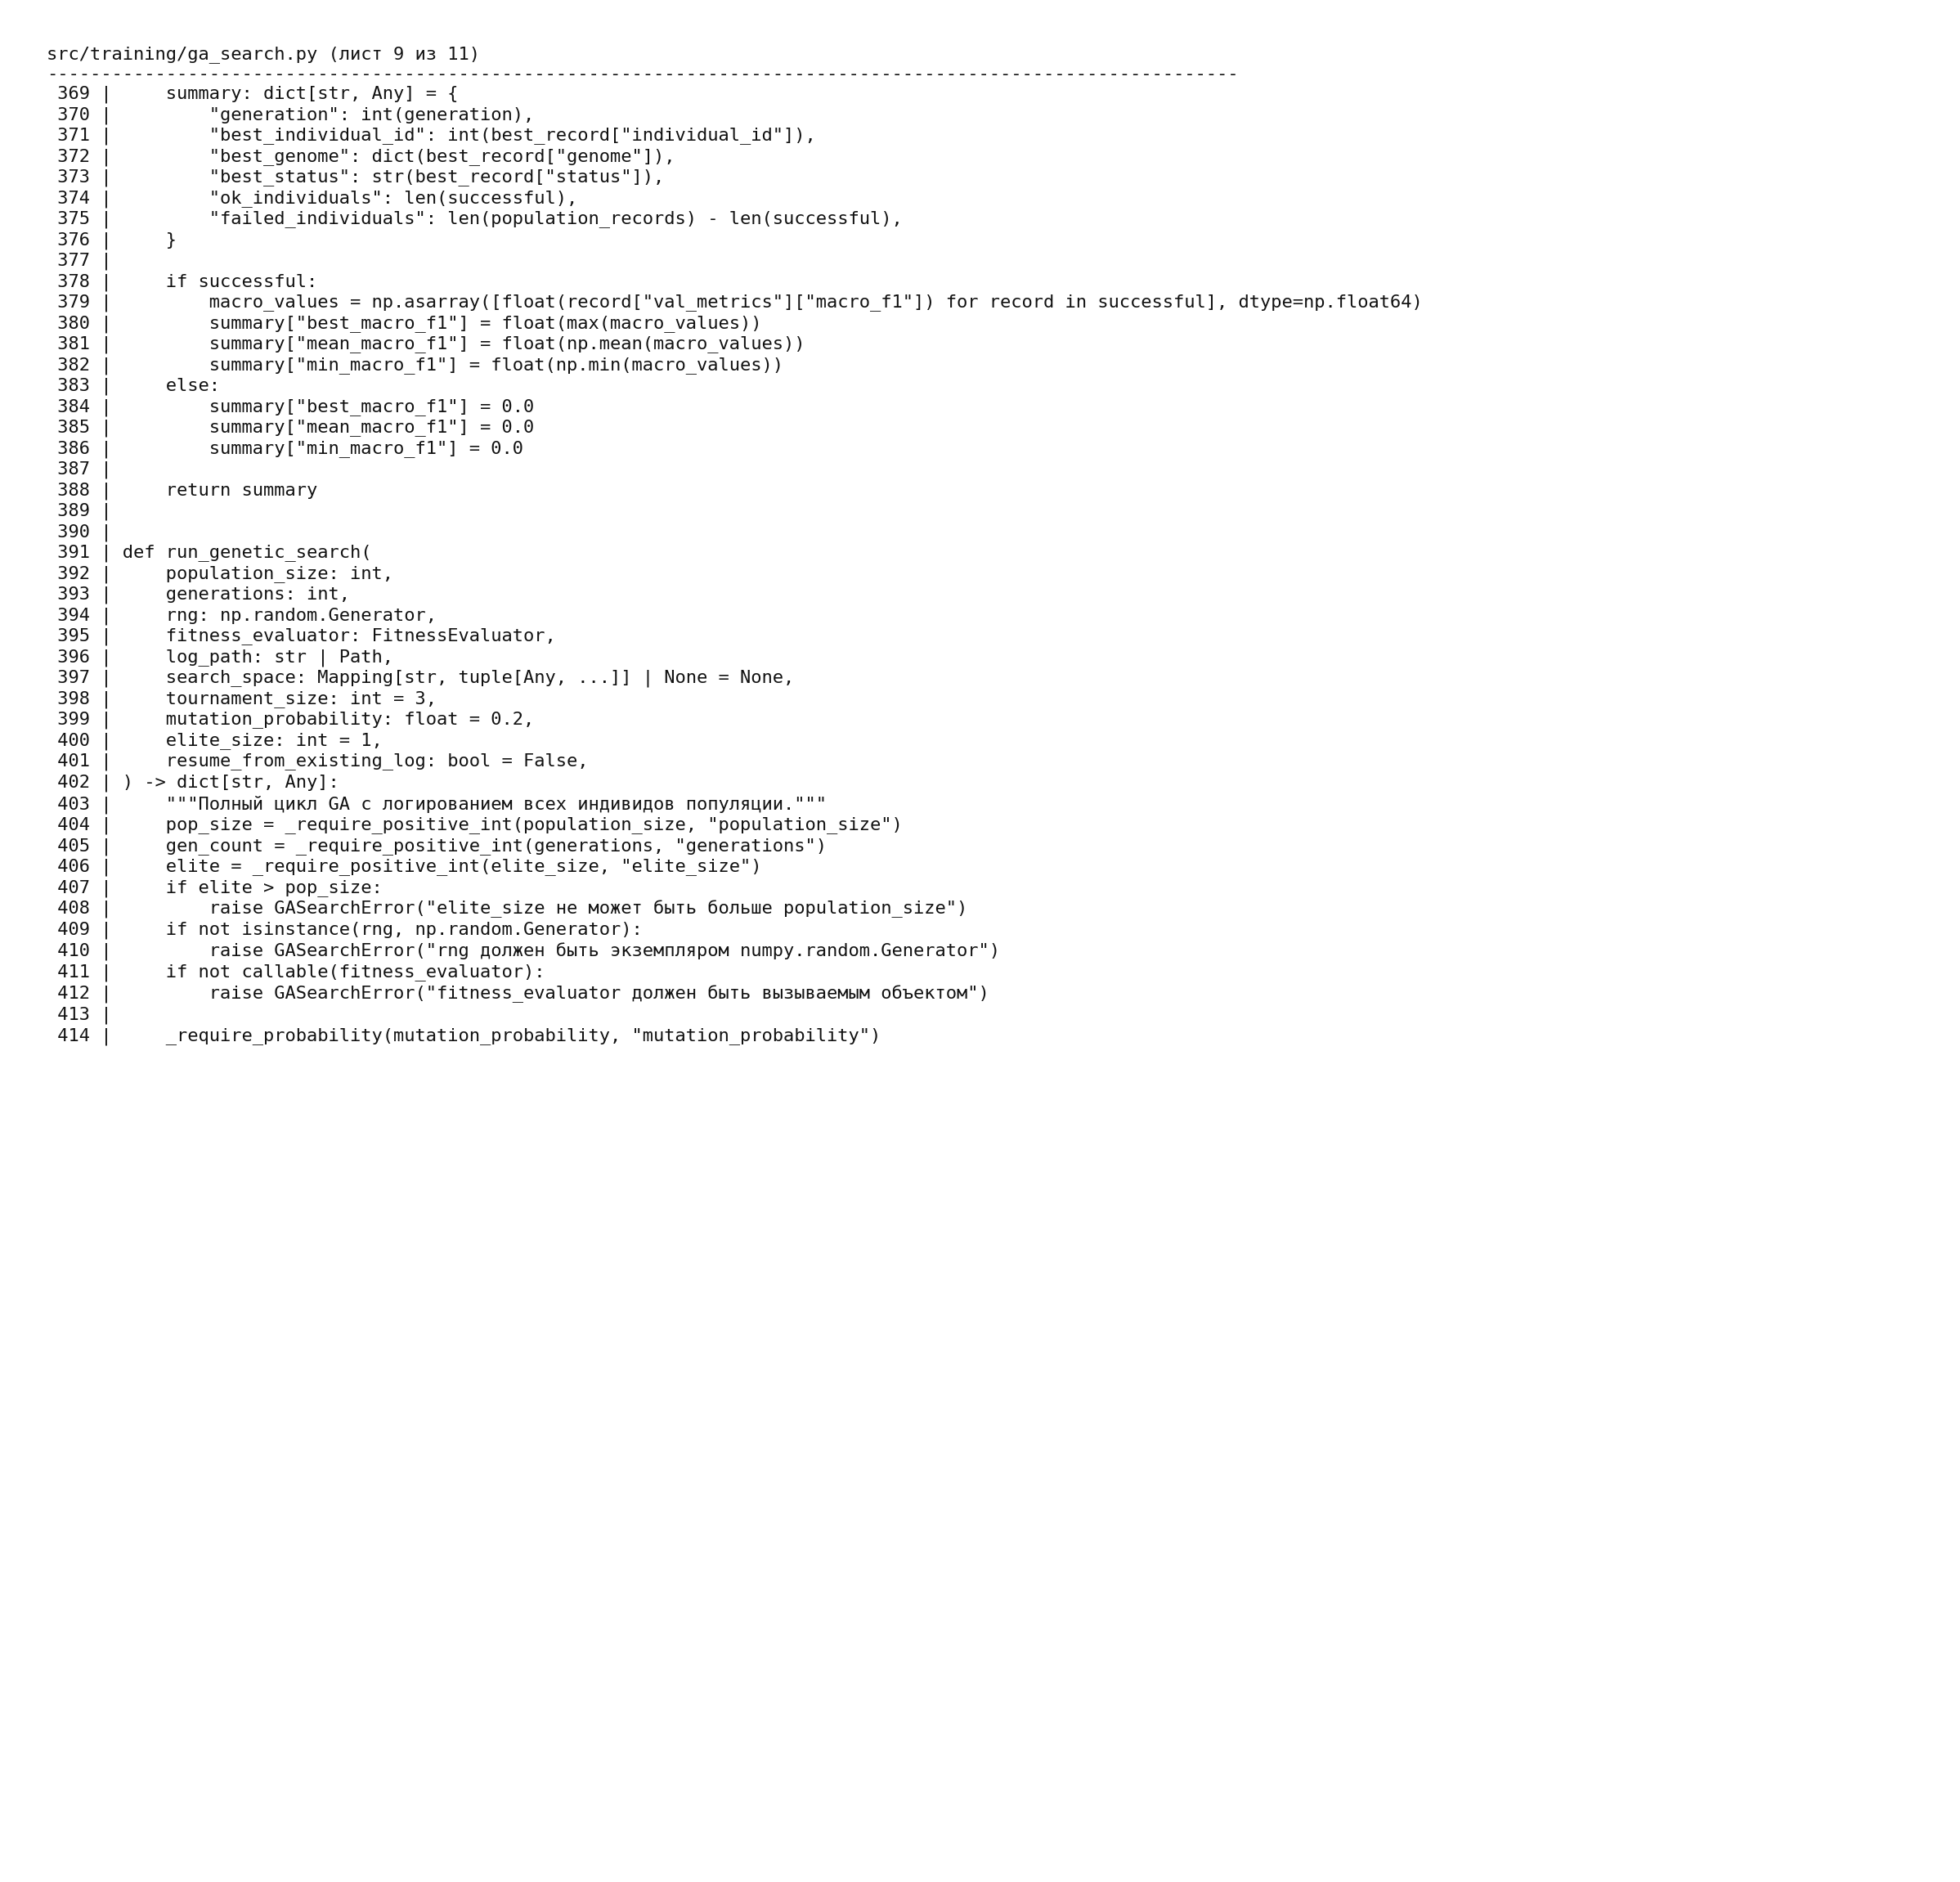
\includegraphics[width=\textwidth]{figures/appendix_ga_p09.png}
\caption{Листинг файла src/training/ga\_search.py, лист 9}
\end{figure}
\begin{figure}[H]
\centering
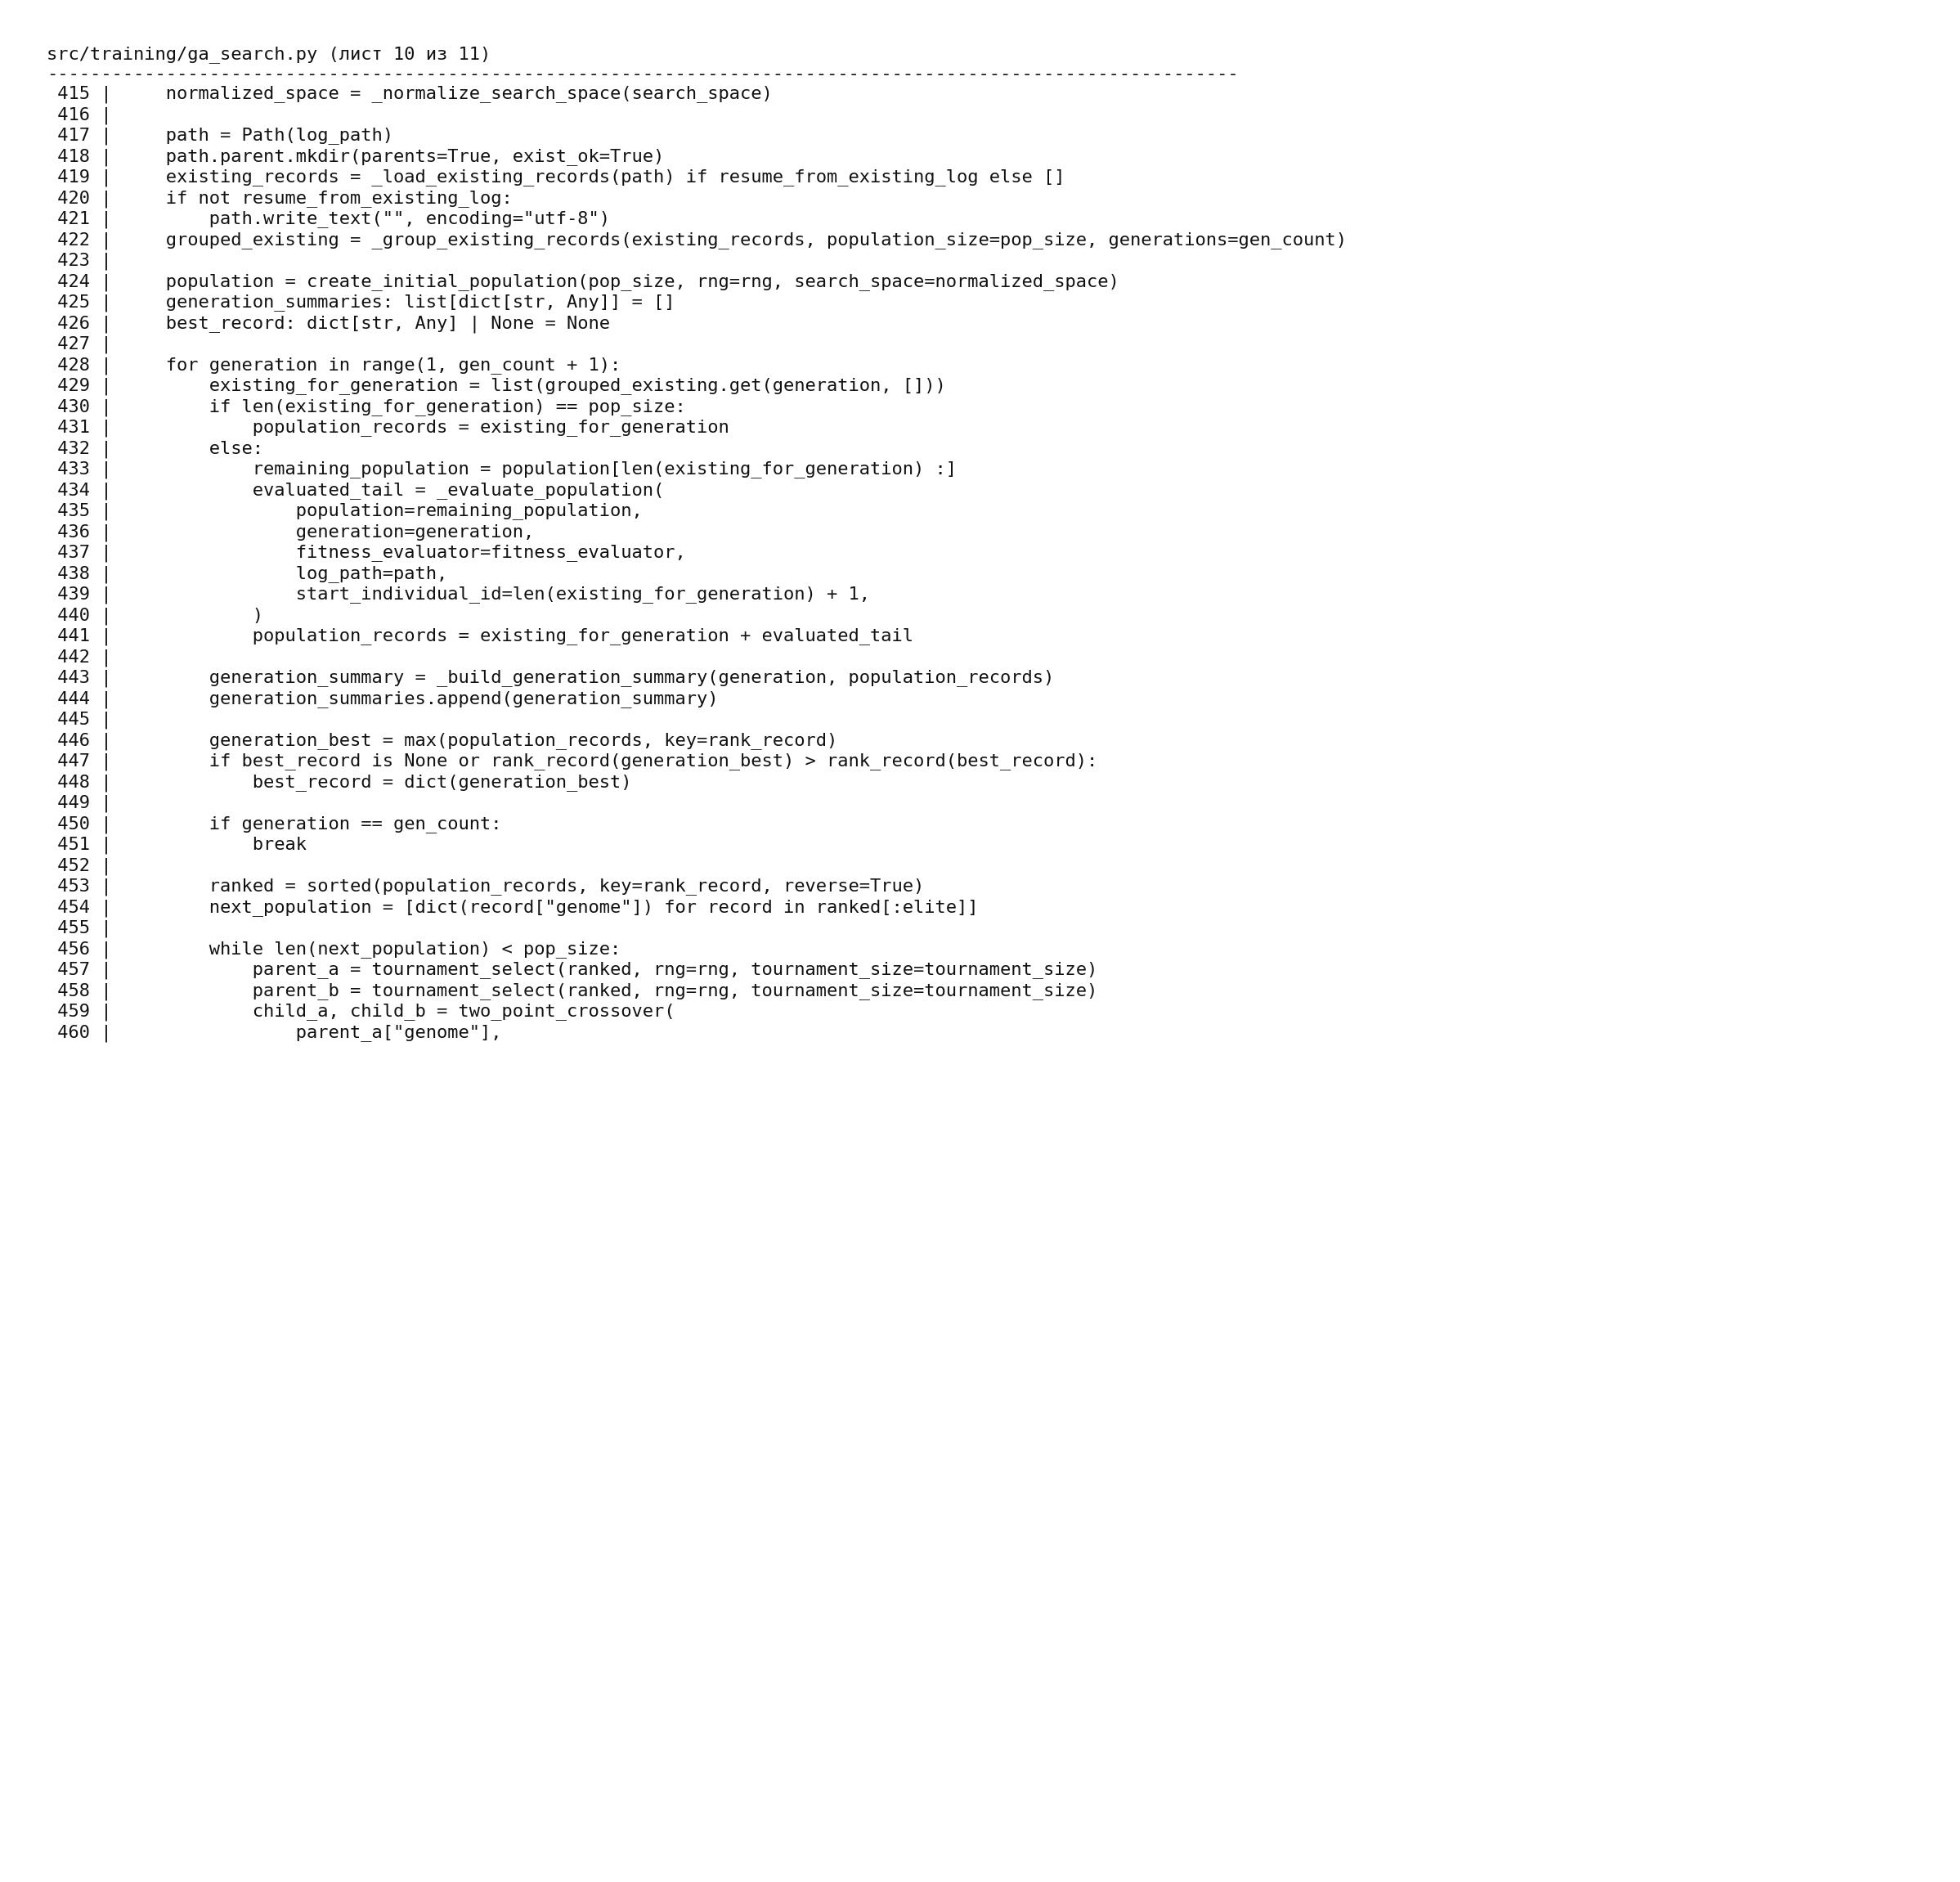
\includegraphics[width=\textwidth]{figures/appendix_ga_p10.png}
\caption{Листинг файла src/training/ga\_search.py, лист 10}
\end{figure}
\begin{figure}[H]
\centering
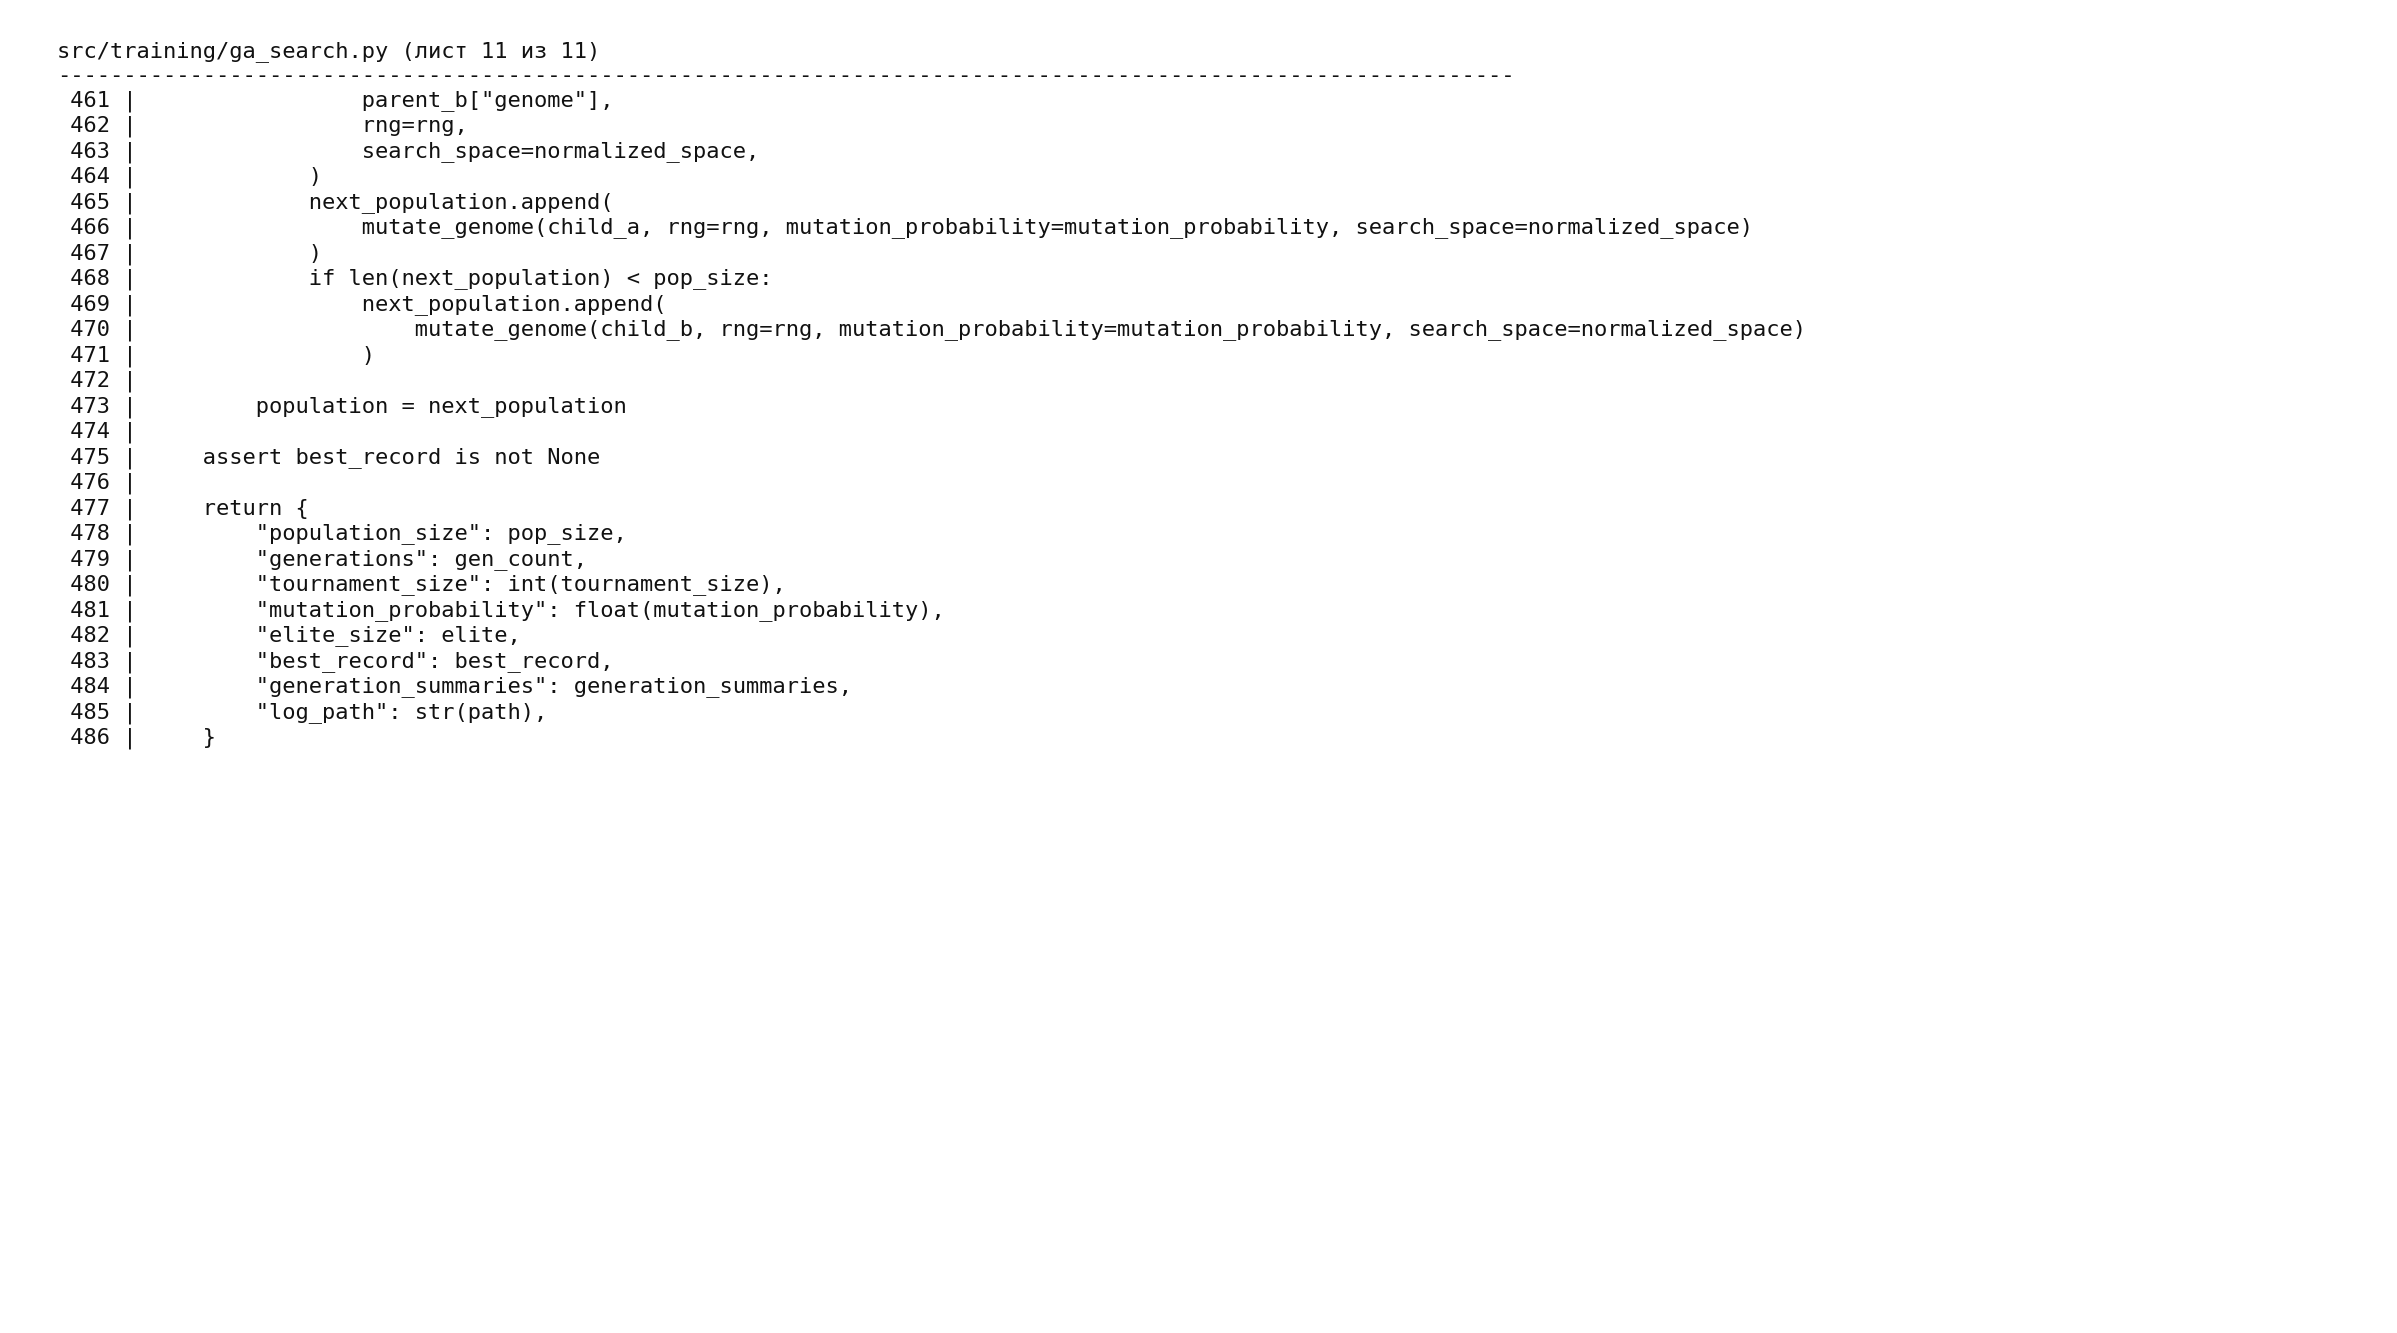
\includegraphics[width=\textwidth]{figures/appendix_ga_p11.png}
\caption{Листинг файла src/training/ga\_search.py, лист 11}
\end{figure}
\clearpage
\section*{Приложение Г. Автоэнкодер и перенос весов энкодера}
\addcontentsline{toc}{section}{Приложение Г. Автоэнкодер и перенос весов энкодера}
\noindent\textbf{Файл:} \path{src/models/autoencoder.py}
\par\vspace{0.4cm}
\begin{figure}[H]
\centering
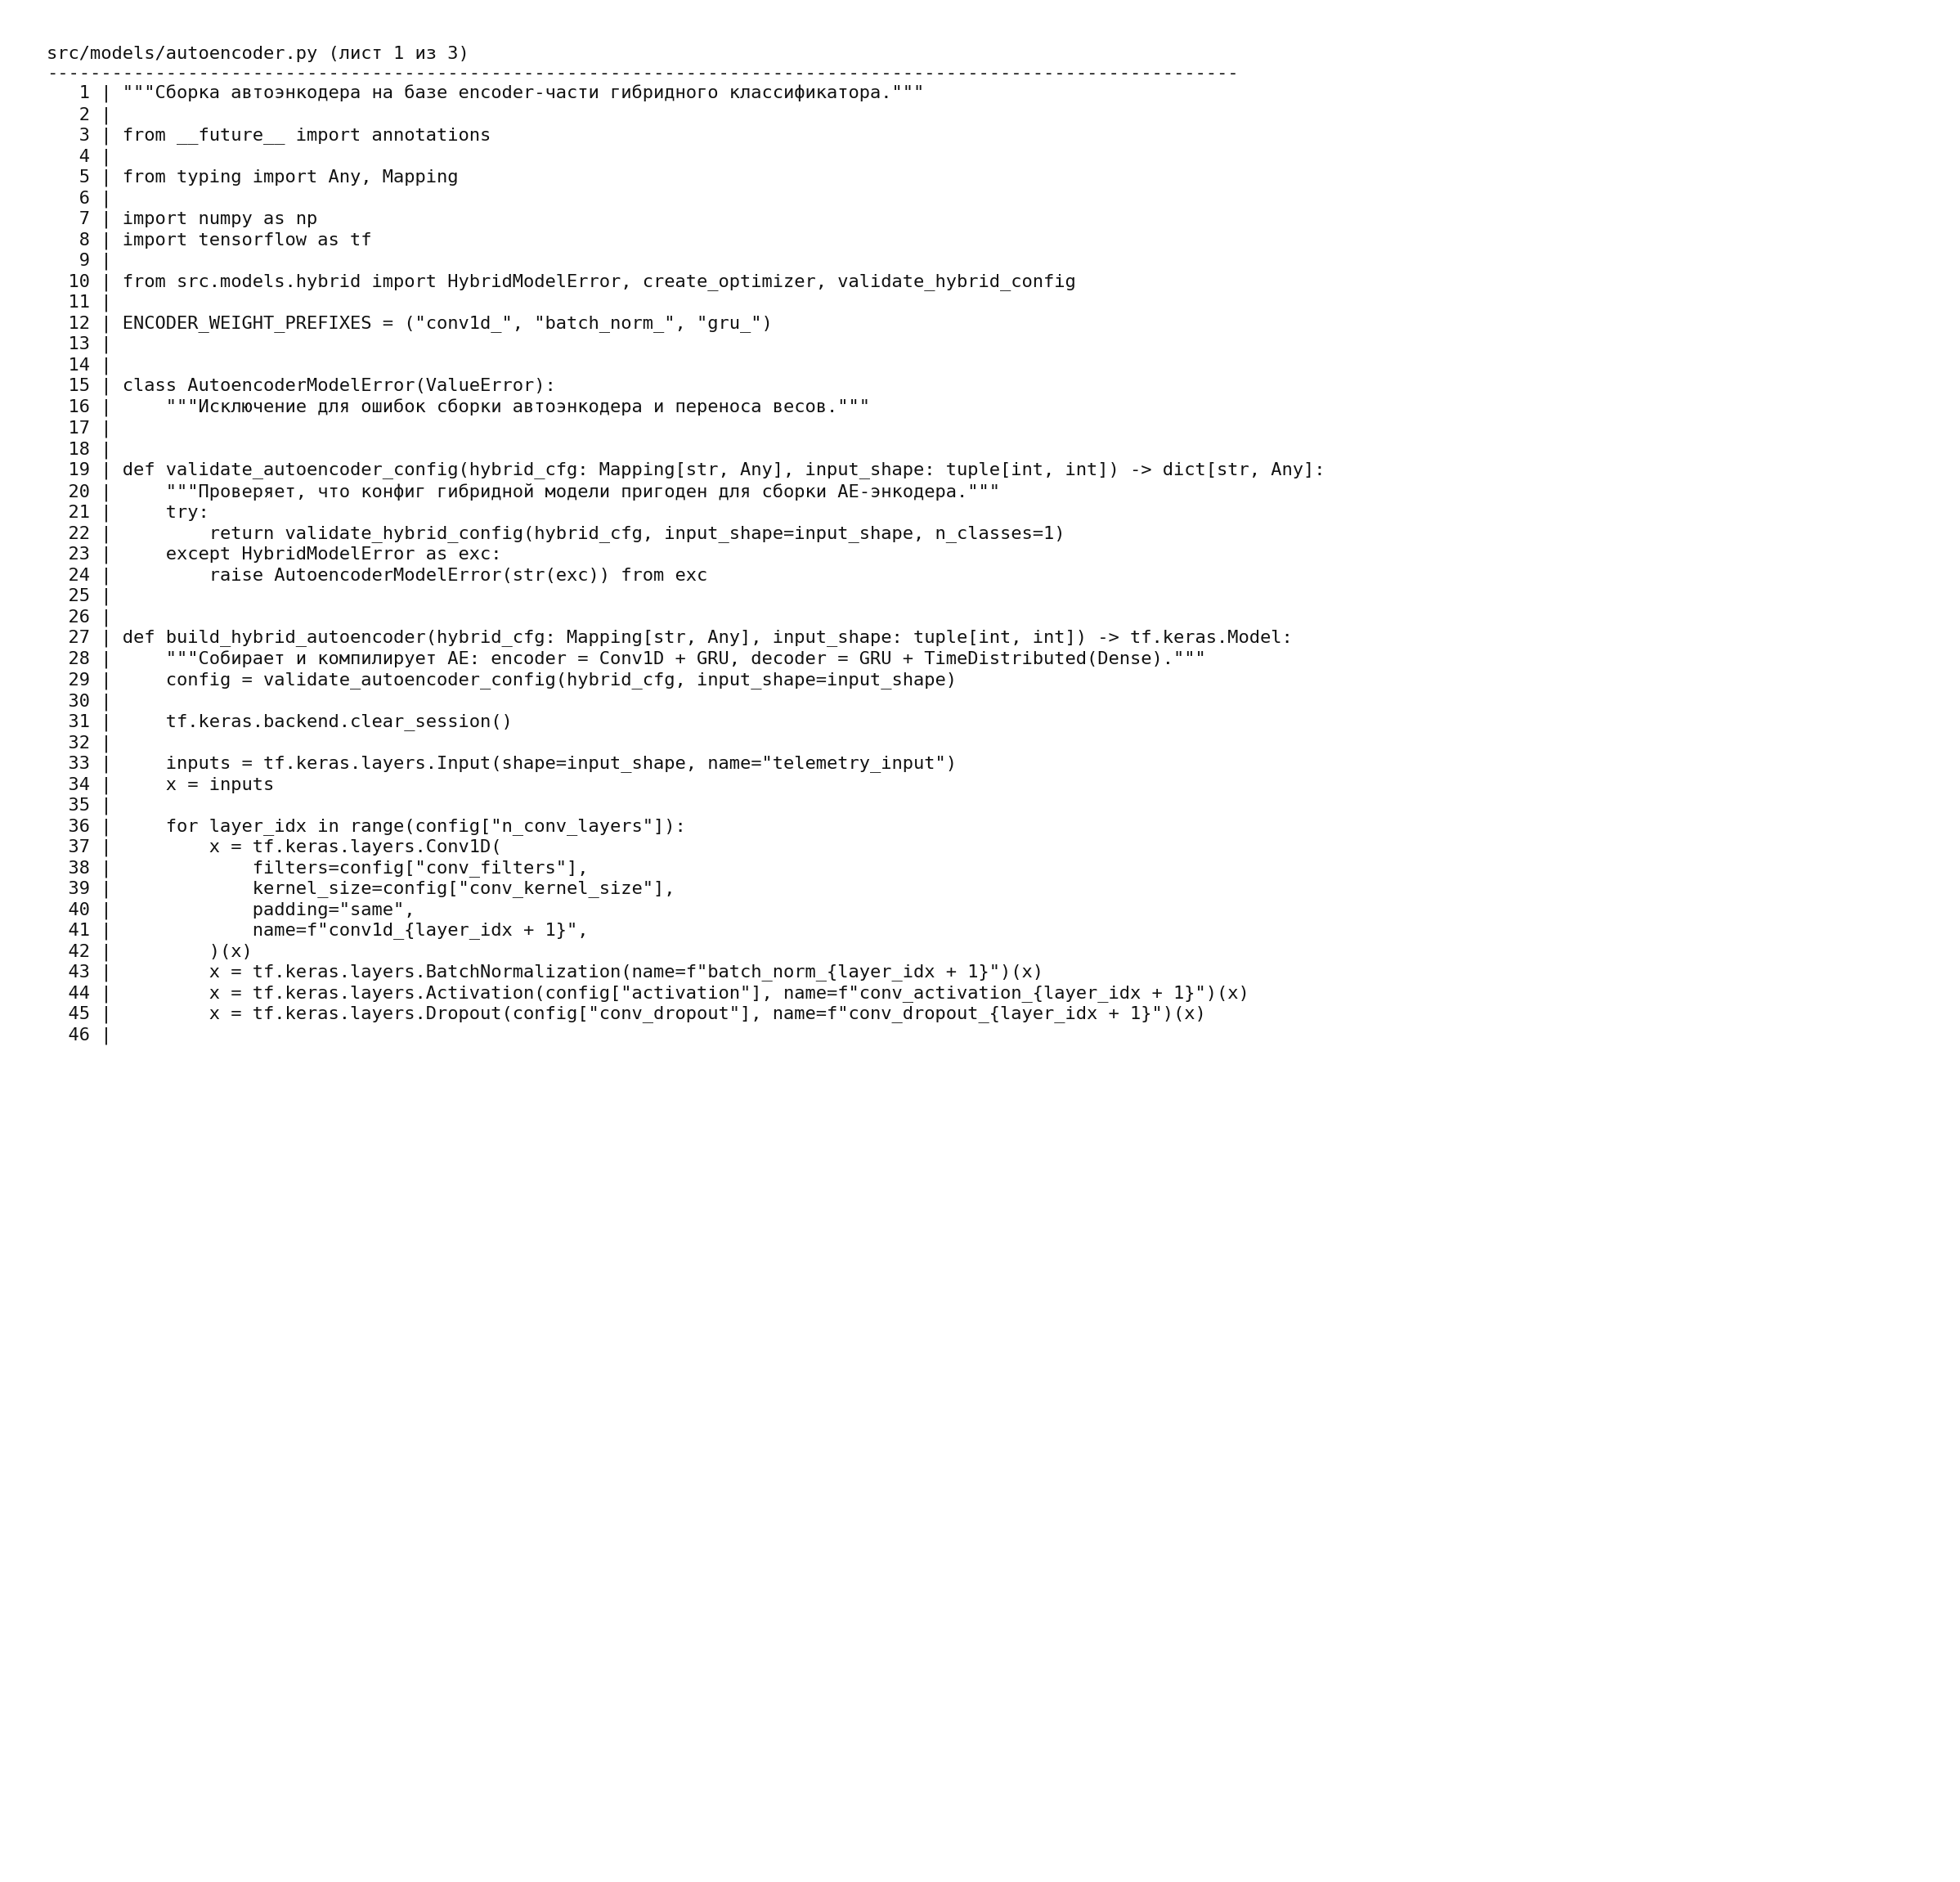
\includegraphics[width=\textwidth]{figures/appendix_autoencoder_p01.png}
\caption{Листинг файла src/models/autoencoder.py, лист 1}
\end{figure}
\begin{figure}[H]
\centering
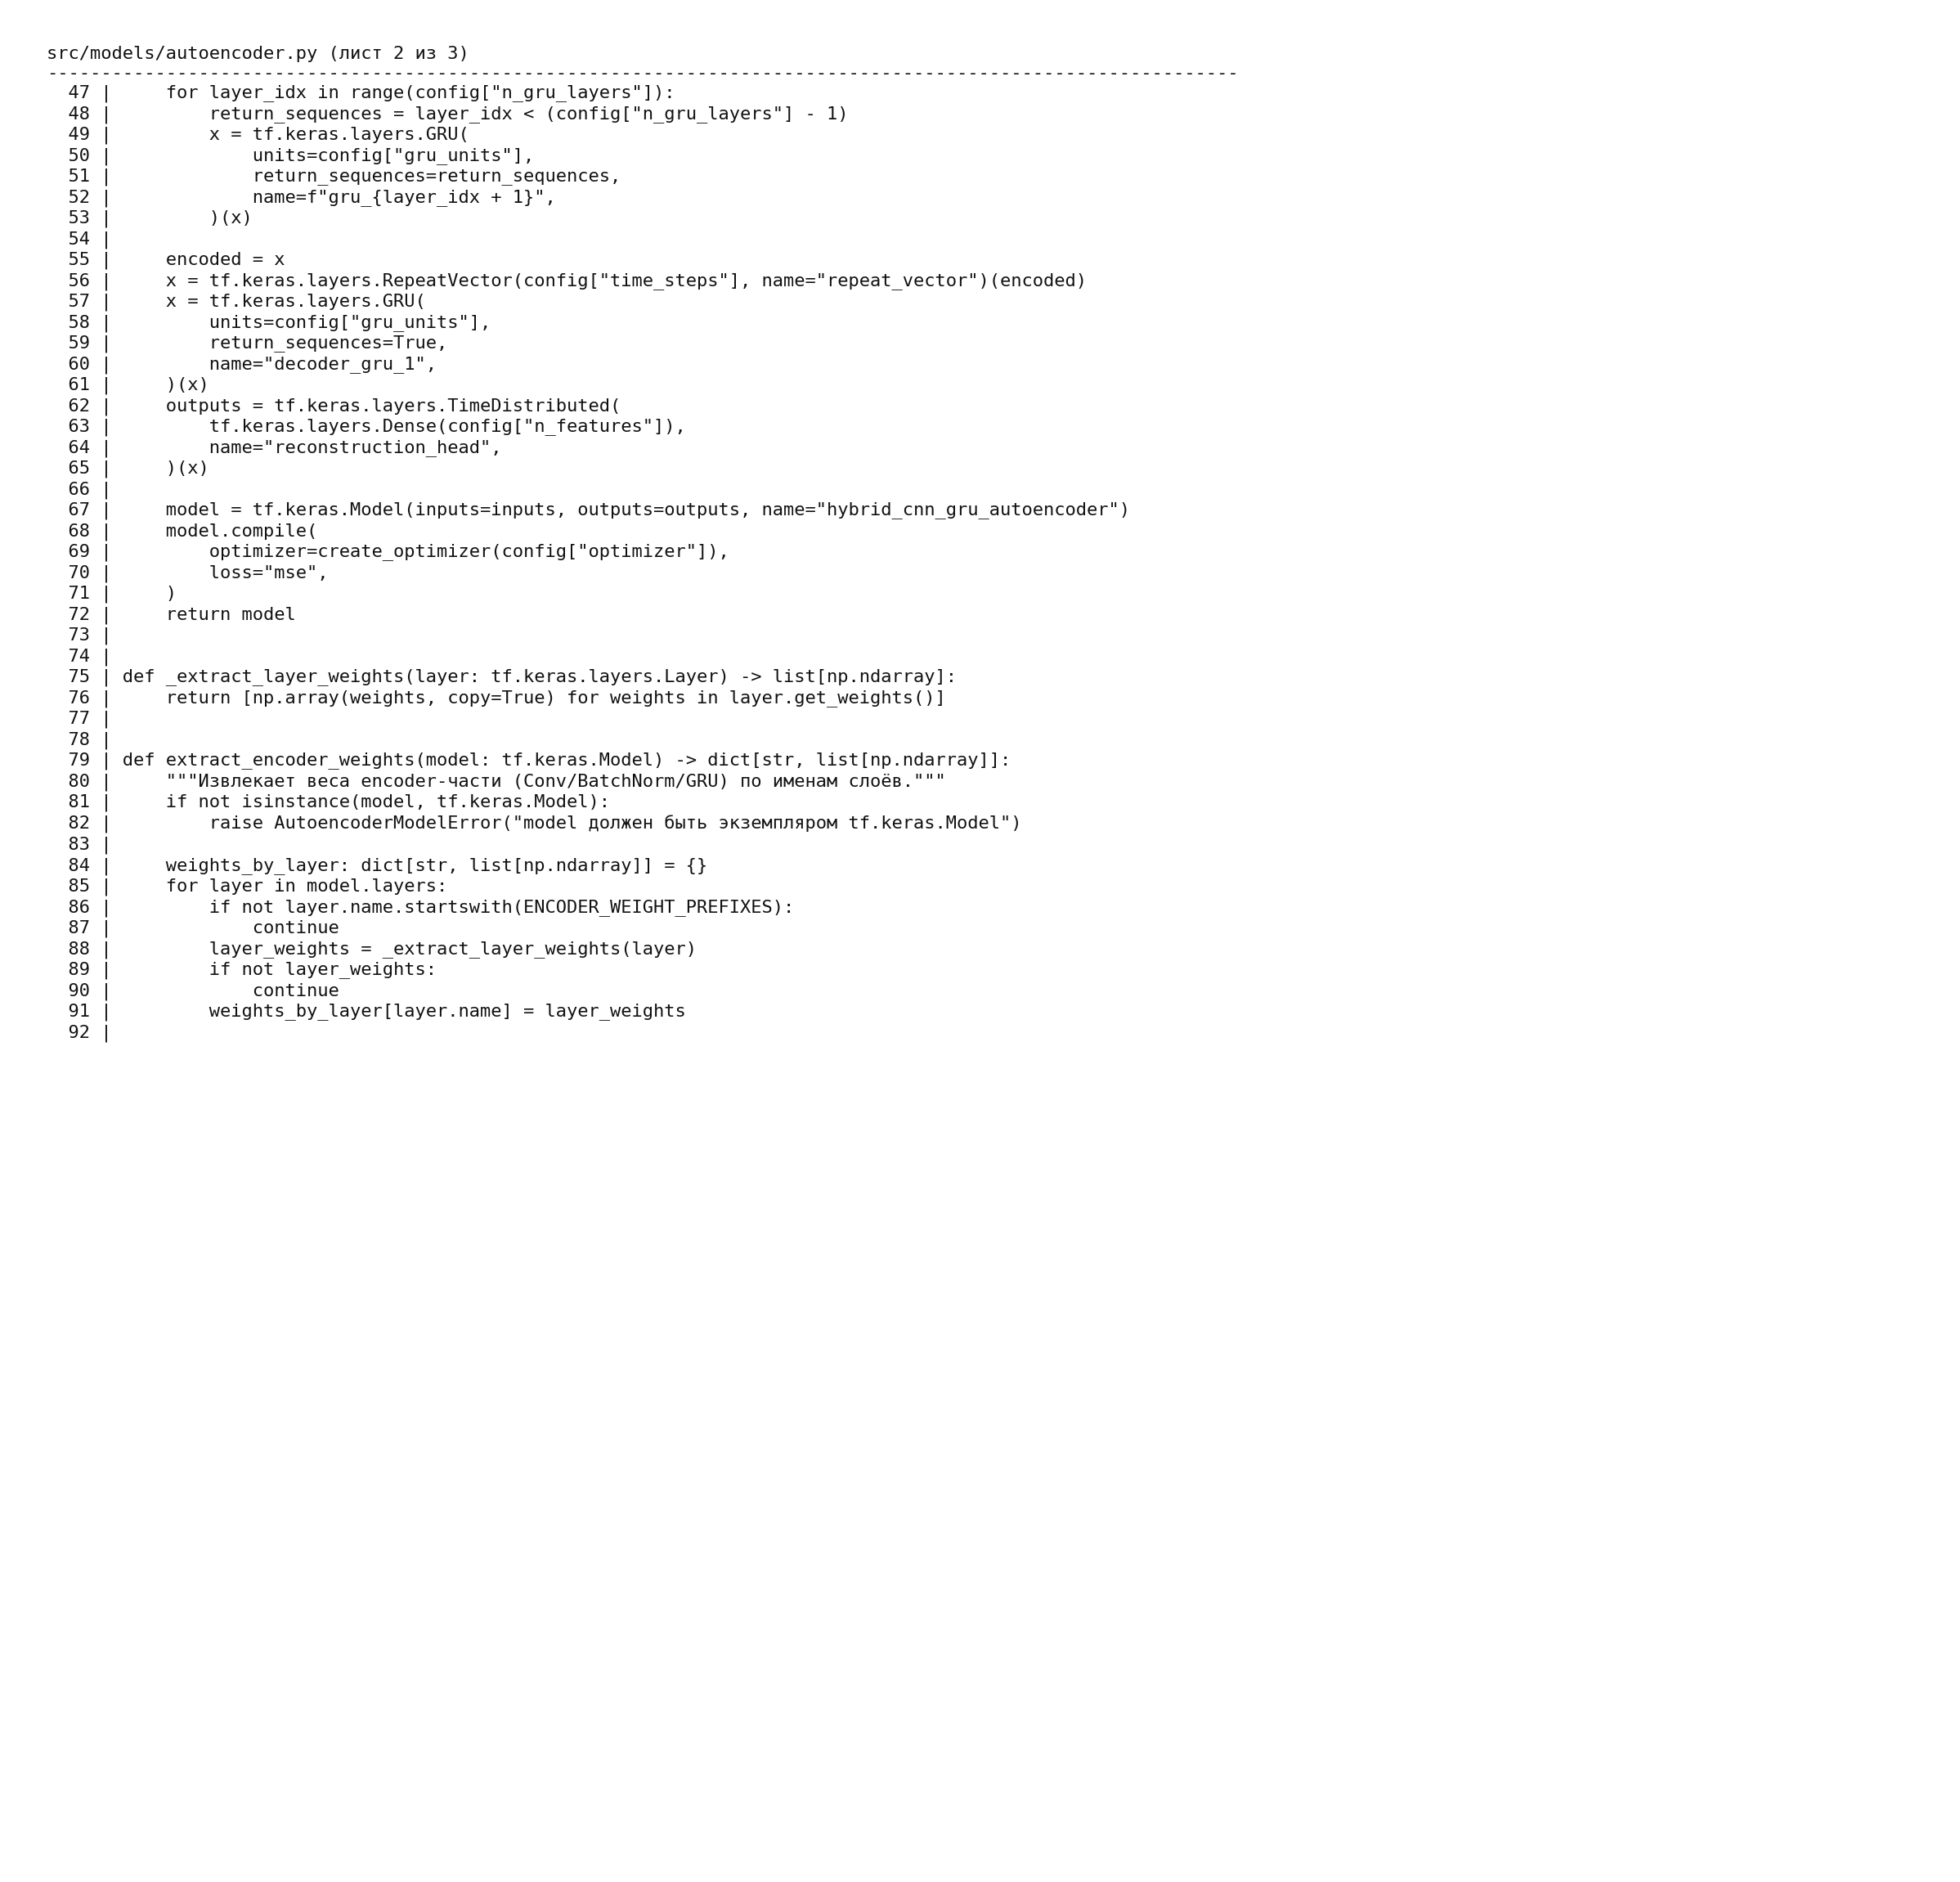
\includegraphics[width=\textwidth]{figures/appendix_autoencoder_p02.png}
\caption{Листинг файла src/models/autoencoder.py, лист 2}
\end{figure}
\begin{figure}[H]
\centering
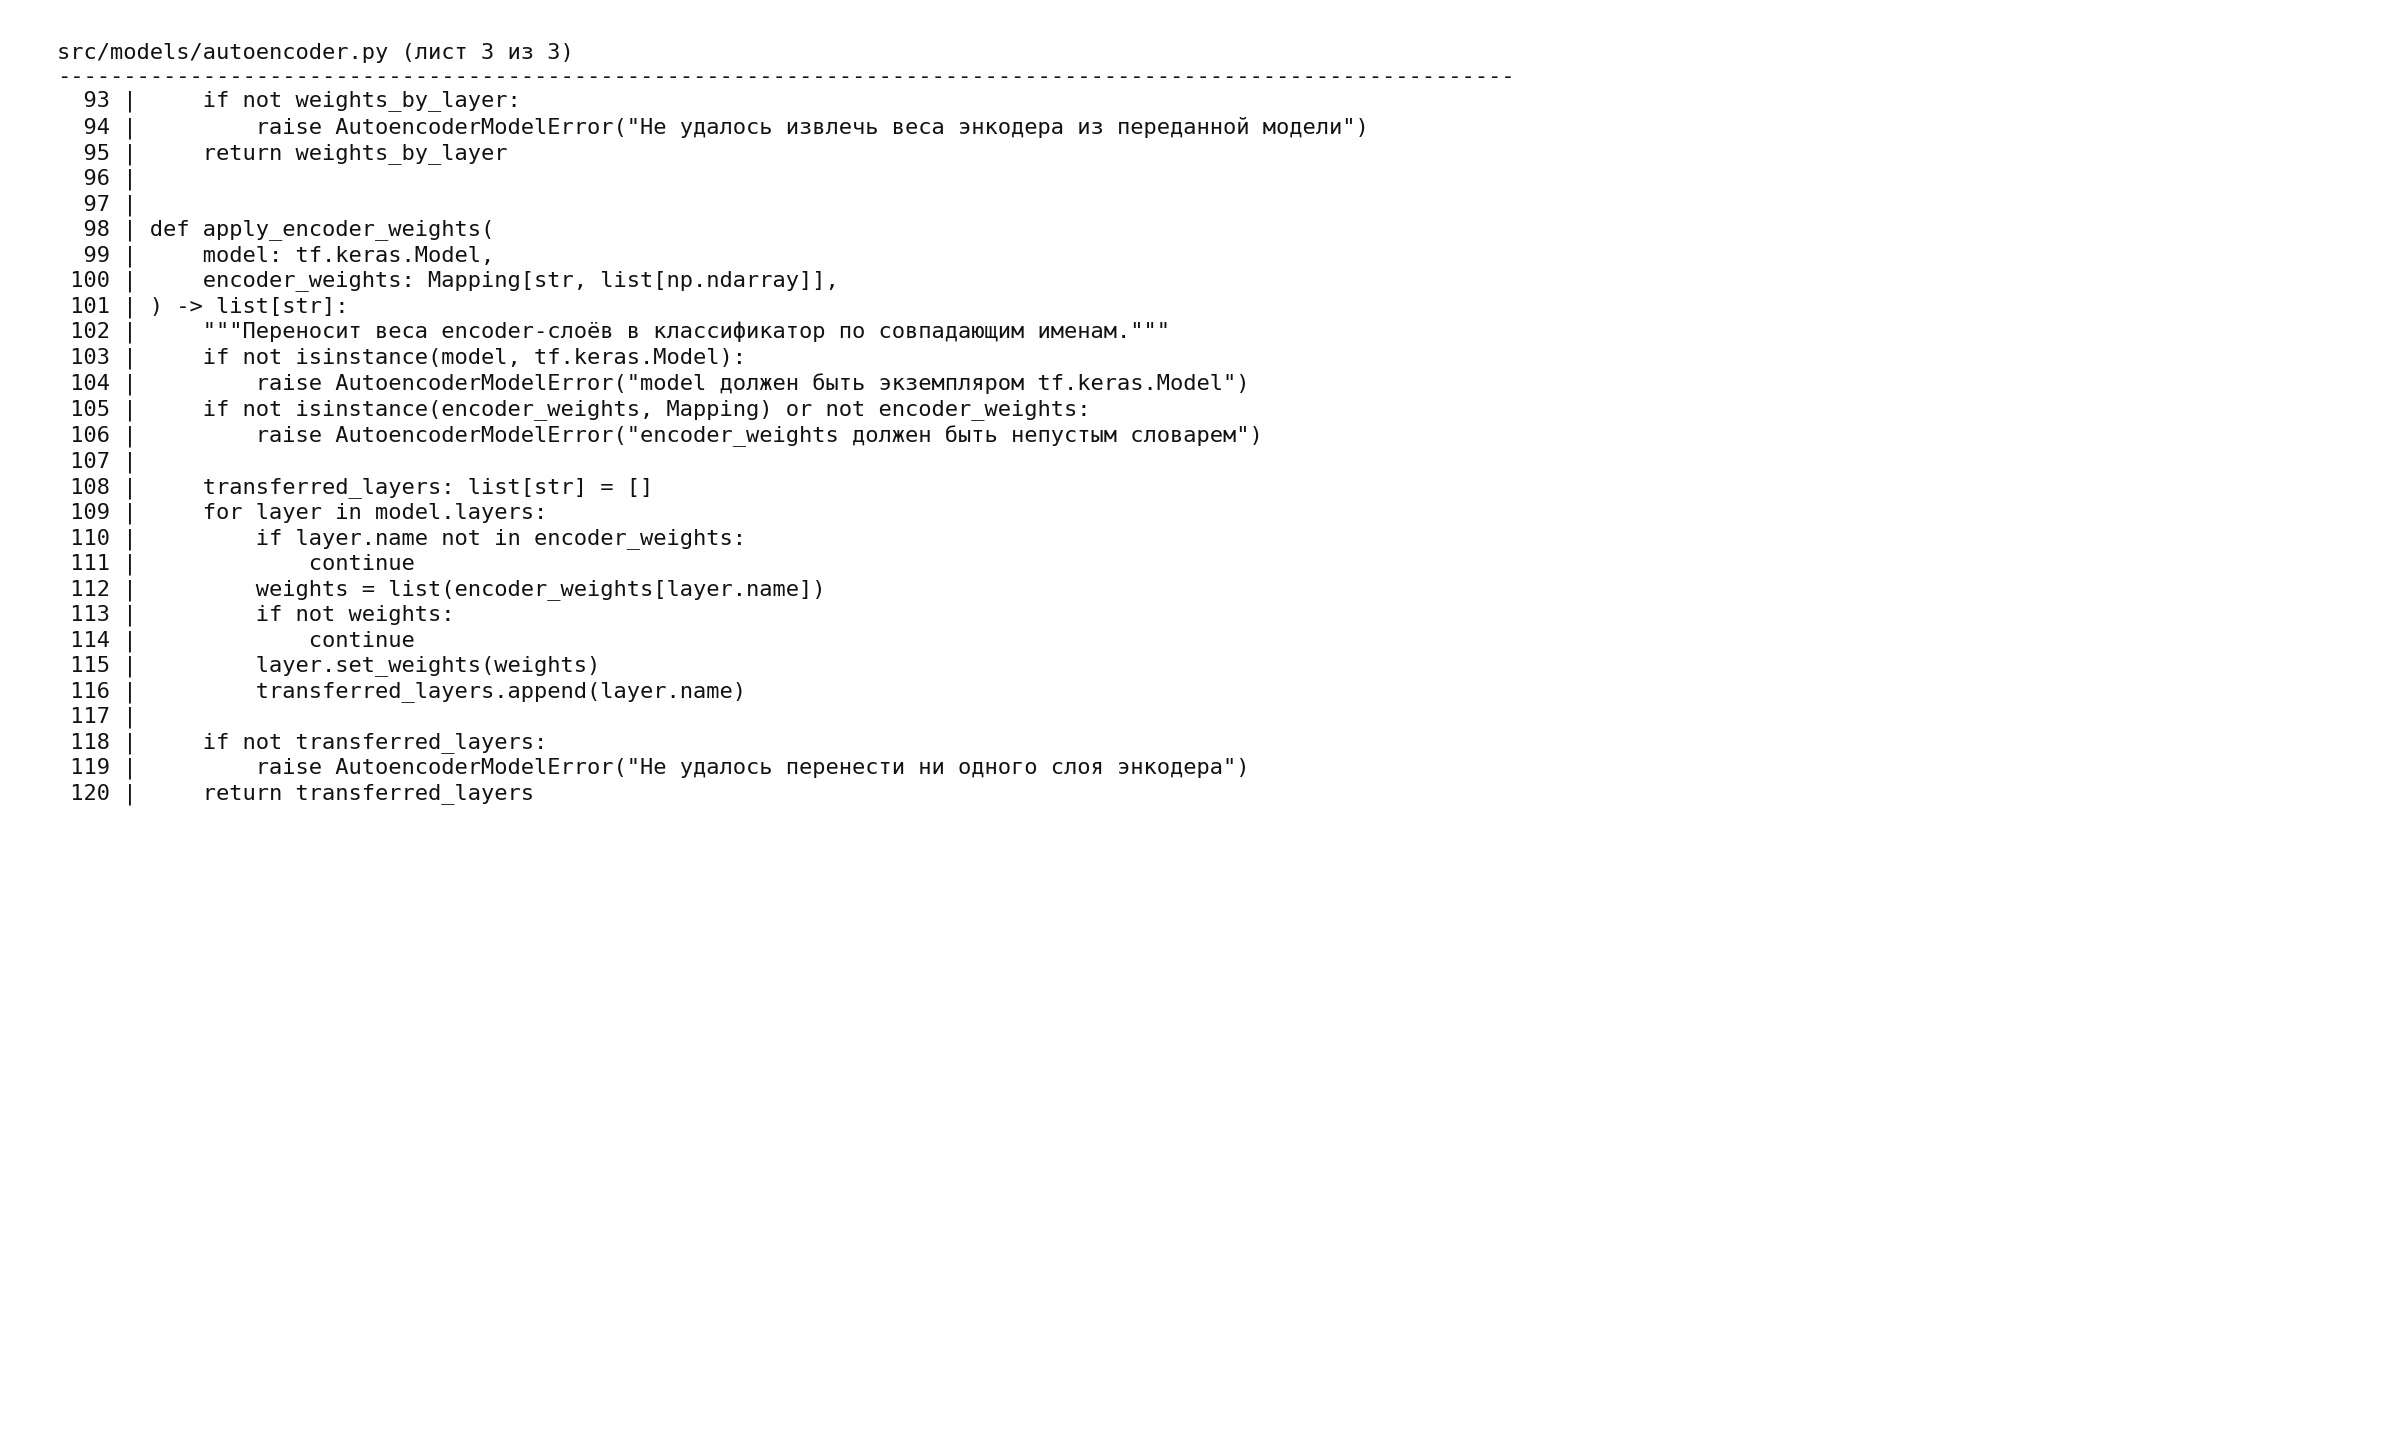
\includegraphics[width=\textwidth]{figures/appendix_autoencoder_p03.png}
\caption{Листинг файла src/models/autoencoder.py, лист 3}
\end{figure}
\clearpage
}{\textit{Файл с приложениями кода не найден.}}

\end{document}
